%% Ngân hàng đề Toán 12 (KNTT) -- Chương I, Bài 1, Dạng 05
%% Dạng: Đọc đồ thị hoặc dấu của $f'(x)$ để xét tính đơn điệu, cực trị
%% Phương án ĐẦU TIÊN trong \cauTN luôn là đáp án đúng (gói trondethi tự đảo).
%% Phần II: \y{nội dung}{d|s}. Phần III: đáp án đặt ở đối số cuối.

\cauTN[id=C1-B1-D05-NB-001,muc=NB,loigiai={Từ bảng xét dấu, $f'(x)<0$ trên $(-\infty;-3)$, $(-2;+\infty)$ nên hàm số nghịch biến trên các khoảng đó.}]{Cho hàm số $y=f(x)$ có bảng xét dấu của đạo hàm như sau:
\begin{center}
\begin{tikzpicture}
\tkzTabInit[lgt=1.4,espcl=2.0]{$x$/0.7,$f'(x)$/0.7}{$-\infty$,$-3$,$-2$,$+\infty$}
\tkzTabLine{ ,-,z,+,z,-, }
\end{tikzpicture}
\end{center}
Hàm số đã cho nghịch biến trên khoảng nào dưới đây?}
  {$(-2;+\infty)$.}
  {$(-3;-2)$.}{$(-\infty;-2)$.}{$(-3;+\infty)$.}

\cauTN[id=C1-B1-D05-NB-002,muc=NB,loigiai={Từ bảng xét dấu, $f'(x)<0$ trên $(-\infty;-2)$, $(0;3)$ nên hàm số nghịch biến trên các khoảng đó.}]{Cho hàm số $y=f(x)$ có bảng xét dấu của đạo hàm như sau:
\begin{center}
\begin{tikzpicture}
\tkzTabInit[lgt=1.4,espcl=2.0]{$x$/0.7,$f'(x)$/0.7}{$-\infty$,$-2$,$0$,$3$,$+\infty$}
\tkzTabLine{ ,-,z,+,z,-,z,+, }
\end{tikzpicture}
\end{center}
Hàm số đã cho nghịch biến trên khoảng nào dưới đây?}
  {$(-\infty;-2)$.}
  {$(-2;0)$.}{$(3;+\infty)$.}{$(-\infty;0)$.}

\cauTN[id=C1-B1-D05-NB-003,muc=NB,loigiai={Từ bảng xét dấu, $f'(x)>0$ trên $(0;4)$ nên hàm số đồng biến trên các khoảng đó.}]{Cho hàm số $y=f(x)$ có bảng xét dấu của đạo hàm như sau:
\begin{center}
\begin{tikzpicture}
\tkzTabInit[lgt=1.4,espcl=2.0]{$x$/0.7,$f'(x)$/0.7}{$-\infty$,$0$,$4$,$+\infty$}
\tkzTabLine{ ,-,z,+,z,-, }
\end{tikzpicture}
\end{center}
Hàm số đã cho đồng biến trên khoảng nào dưới đây?}
  {$(0;4)$.}
  {$(-\infty;0)$.}{$(4;+\infty)$.}{$(-\infty;4)$.}

\cauTN[id=C1-B1-D05-NB-004,muc=NB,loigiai={Từ bảng xét dấu, $f'(x)<0$ trên $(-\infty;-2)$, $(3;+\infty)$ nên hàm số nghịch biến trên các khoảng đó.}]{Cho hàm số $y=f(x)$ có bảng xét dấu của đạo hàm như sau:
\begin{center}
\begin{tikzpicture}
\tkzTabInit[lgt=1.4,espcl=2.0]{$x$/0.7,$f'(x)$/0.7}{$-\infty$,$-2$,$3$,$+\infty$}
\tkzTabLine{ ,-,z,+,z,-, }
\end{tikzpicture}
\end{center}
Hàm số đã cho nghịch biến trên khoảng nào dưới đây?}
  {$(3;+\infty)$.}
  {$(-2;3)$.}{$(-\infty;3)$.}{$(-2;+\infty)$.}

\cauTN[id=C1-B1-D05-NB-005,muc=NB,loigiai={Từ bảng xét dấu, $f'(x)>0$ trên $(0;3)$ nên hàm số đồng biến trên các khoảng đó.}]{Cho hàm số $y=f(x)$ có bảng xét dấu của đạo hàm như sau:
\begin{center}
\begin{tikzpicture}
\tkzTabInit[lgt=1.4,espcl=2.0]{$x$/0.7,$f'(x)$/0.7}{$-\infty$,$0$,$3$,$+\infty$}
\tkzTabLine{ ,-,z,+,z,-, }
\end{tikzpicture}
\end{center}
Hàm số đã cho đồng biến trên khoảng nào dưới đây?}
  {$(0;3)$.}
  {$(-\infty;0)$.}{$(3;+\infty)$.}{$(-\infty;3)$.}

\cauTN[id=C1-B1-D05-NB-006,muc=NB,loigiai={$f'(x)$ đổi dấu từ dương sang âm khi qua $x=4$ nên hàm số đạt cực đại tại đó.}]{Cho hàm số $y=f(x)$ có bảng xét dấu của đạo hàm như sau:
\begin{center}
\begin{tikzpicture}
\tkzTabInit[lgt=1.4,espcl=2.0]{$x$/0.7,$f'(x)$/0.7}{$-\infty$,$3$,$4$,$+\infty$}
\tkzTabLine{ ,-,z,+,z,-, }
\end{tikzpicture}
\end{center}
Hàm số đã cho đạt cực đại tại điểm nào dưới đây?}
  {$x=4$.}
  {$x=3$.}{$x=5$.}{$x=-4$.}

\cauTN[id=C1-B1-D05-NB-007,muc=NB,loigiai={Từ bảng xét dấu, $f'(x)>0$ trên $(-\infty;-3)$, $(-1;+\infty)$ nên hàm số đồng biến trên các khoảng đó.}]{Cho hàm số $y=f(x)$ có bảng xét dấu của đạo hàm như sau:
\begin{center}
\begin{tikzpicture}
\tkzTabInit[lgt=1.4,espcl=2.0]{$x$/0.7,$f'(x)$/0.7}{$-\infty$,$-3$,$-1$,$+\infty$}
\tkzTabLine{ ,+,z,-,z,+, }
\end{tikzpicture}
\end{center}
Hàm số đã cho đồng biến trên khoảng nào dưới đây?}
  {$(-\infty;-3)$.}
  {$(-3;-1)$.}{$(-\infty;-1)$.}{$(-3;+\infty)$.}

\cauTN[id=C1-B1-D05-NB-008,muc=NB,loigiai={$f'(x)$ đổi dấu từ dương sang âm khi qua $x=4$ nên hàm số đạt cực đại tại đó.}]{Cho hàm số $y=f(x)$ có bảng xét dấu của đạo hàm như sau:
\begin{center}
\begin{tikzpicture}
\tkzTabInit[lgt=1.4,espcl=2.0]{$x$/0.7,$f'(x)$/0.7}{$-\infty$,$-3$,$4$,$+\infty$}
\tkzTabLine{ ,-,z,+,z,-, }
\end{tikzpicture}
\end{center}
Hàm số đã cho đạt cực đại tại điểm nào dưới đây?}
  {$x=4$.}
  {$x=-3$.}{$x=5$.}{$x=-4$.}

\cauTN[id=C1-B1-D05-NB-009,muc=NB,loigiai={$f'(x)$ đổi dấu từ dương sang âm khi qua $x=-2$ nên hàm số đạt cực đại tại đó.}]{Cho hàm số $y=f(x)$ có bảng xét dấu của đạo hàm như sau:
\begin{center}
\begin{tikzpicture}
\tkzTabInit[lgt=1.4,espcl=2.0]{$x$/0.7,$f'(x)$/0.7}{$-\infty$,$-4$,$-2$,$-1$,$+\infty$}
\tkzTabLine{ ,-,z,+,z,-,z,+, }
\end{tikzpicture}
\end{center}
Hàm số đã cho đạt cực đại tại điểm nào dưới đây?}
  {$x=-2$.}
  {$x=-4$.}{$x=-1$.}{$x=2$.}

\cauTN[id=C1-B1-D05-NB-010,muc=NB,loigiai={Từ bảng xét dấu, $f'(x)<0$ trên $(-2;0)$, $(2;+\infty)$ nên hàm số nghịch biến trên các khoảng đó.}]{Cho hàm số $y=f(x)$ có bảng xét dấu của đạo hàm như sau:
\begin{center}
\begin{tikzpicture}
\tkzTabInit[lgt=1.4,espcl=2.0]{$x$/0.7,$f'(x)$/0.7}{$-\infty$,$-2$,$0$,$2$,$+\infty$}
\tkzTabLine{ ,+,z,-,z,+,z,-, }
\end{tikzpicture}
\end{center}
Hàm số đã cho nghịch biến trên khoảng nào dưới đây?}
  {$(-2;0)$.}
  {$(-\infty;-2)$.}{$(0;2)$.}{$(-\infty;0)$.}

\cauTN[id=C1-B1-D05-NB-011,muc=NB,loigiai={Từ bảng xét dấu, $f'(x)<0$ trên $(-4;2)$ nên hàm số nghịch biến trên các khoảng đó.}]{Cho hàm số $y=f(x)$ có bảng xét dấu của đạo hàm như sau:
\begin{center}
\begin{tikzpicture}
\tkzTabInit[lgt=1.4,espcl=2.0]{$x$/0.7,$f'(x)$/0.7}{$-\infty$,$-4$,$2$,$+\infty$}
\tkzTabLine{ ,+,z,-,z,+, }
\end{tikzpicture}
\end{center}
Hàm số đã cho nghịch biến trên khoảng nào dưới đây?}
  {$(-4;2)$.}
  {$(-\infty;-4)$.}{$(2;+\infty)$.}{$(-\infty;2)$.}

\cauTN[id=C1-B1-D05-NB-012,muc=NB,loigiai={$f'(x)$ đổi dấu từ dương sang âm khi qua $x=1$ nên hàm số đạt cực đại tại đó.}]{Cho hàm số $y=f(x)$ có bảng xét dấu của đạo hàm như sau:
\begin{center}
\begin{tikzpicture}
\tkzTabInit[lgt=1.4,espcl=2.0]{$x$/0.7,$f'(x)$/0.7}{$-\infty$,$-3$,$1$,$3$,$+\infty$}
\tkzTabLine{ ,-,z,+,z,-,z,+, }
\end{tikzpicture}
\end{center}
Hàm số đã cho đạt cực đại tại điểm nào dưới đây?}
  {$x=1$.}
  {$x=-3$.}{$x=3$.}{$x=2$.}

\cauTN[id=C1-B1-D05-NB-013,muc=NB,loigiai={Từ bảng xét dấu, $f'(x)>0$ trên $(-3;-2)$ nên hàm số đồng biến trên các khoảng đó.}]{Cho hàm số $y=f(x)$ có bảng xét dấu của đạo hàm như sau:
\begin{center}
\begin{tikzpicture}
\tkzTabInit[lgt=1.4,espcl=2.0]{$x$/0.7,$f'(x)$/0.7}{$-\infty$,$-3$,$-2$,$+\infty$}
\tkzTabLine{ ,-,z,+,z,-, }
\end{tikzpicture}
\end{center}
Hàm số đã cho đồng biến trên khoảng nào dưới đây?}
  {$(-3;-2)$.}
  {$(-\infty;-3)$.}{$(-2;+\infty)$.}{$(-\infty;-2)$.}

\cauTN[id=C1-B1-D05-NB-014,muc=NB,loigiai={$f'(x)$ đổi dấu từ dương sang âm khi qua $x=-1$ nên hàm số đạt cực đại tại đó.}]{Cho hàm số $y=f(x)$ có bảng xét dấu của đạo hàm như sau:
\begin{center}
\begin{tikzpicture}
\tkzTabInit[lgt=1.4,espcl=2.0]{$x$/0.7,$f'(x)$/0.7}{$-\infty$,$-4$,$-1$,$1$,$+\infty$}
\tkzTabLine{ ,-,z,+,z,-,z,+, }
\end{tikzpicture}
\end{center}
Hàm số đã cho đạt cực đại tại điểm nào dưới đây?}
  {$x=-1$.}
  {$x=-4$.}{$x=1$.}{$x=0$.}

\cauTN[id=C1-B1-D05-NB-015,muc=NB,loigiai={Từ bảng xét dấu: $x=-1$ là điểm cực đại; $x=3$ là điểm cực tiểu; $x=4$ không phải điểm cực trị vì $f'$ không đổi dấu. Vậy kết quả là $2$.}]{Cho hàm số $y=f(x)$ liên tục trên $\mathbb{R}$ và có bảng xét dấu của $f'(x)$ như sau:
\begin{center}
\begin{tikzpicture}
\tkzTabInit[lgt=1.4,espcl=2.0]{$x$/0.7,$f'(x)$/0.7}{$-\infty$,$-1$,$3$,$4$,$+\infty$}
\tkzTabLine{ ,+,z,-,z,+,z,+, }
\end{tikzpicture}
\end{center}
Số điểm cực trị của hàm số đã cho là}
  {$2$.}
  {$3$.}{$1$.}{$4$.}

\cauTN[id=C1-B1-D05-NB-016,muc=NB,loigiai={Từ bảng xét dấu: $x=0$ là điểm cực tiểu ($f'$ không xác định tại đây nhưng $f$ liên tục và $f'$ đổi dấu); $x=1$ không phải điểm cực trị vì $f'$ không đổi dấu; $x=3$ không phải điểm cực trị vì $f'$ không đổi dấu; $x=4$ là điểm cực đại ($f'$ không xác định tại đây nhưng $f$ liên tục và $f'$ đổi dấu). Vậy kết quả là $1$.}]{Cho hàm số $y=f(x)$ liên tục trên $\mathbb{R}$ và có bảng xét dấu của $f'(x)$ như sau:
\begin{center}
\begin{tikzpicture}
\tkzTabInit[lgt=1.4,espcl=2.0]{$x$/0.7,$f'(x)$/0.7}{$-\infty$,$0$,$1$,$3$,$4$,$+\infty$}
\tkzTabLine{ ,-,d,+,z,+,z,+,d,-, }
\end{tikzpicture}
\end{center}
Số điểm cực tiểu của hàm số đã cho là}
  {$1$.}
  {$4$.}{$2$.}{$0$.}

\cauTN[id=C1-B1-D05-NB-017,muc=NB,loigiai={Từ bảng xét dấu: $x=-2$ là điểm cực đại; $x=-1$ là điểm cực tiểu; $x=1$ là điểm cực đại; $x=3$ là điểm cực tiểu ($f'$ không xác định tại đây nhưng $f$ liên tục và $f'$ đổi dấu). Vậy kết quả là $1$.}]{Cho hàm số $y=f(x)$ liên tục trên $\mathbb{R}$ và có bảng xét dấu của $f'(x)$ như sau:
\begin{center}
\begin{tikzpicture}
\tkzTabInit[lgt=1.4,espcl=2.0]{$x$/0.7,$f'(x)$/0.7}{$-\infty$,$-2$,$-1$,$1$,$3$,$+\infty$}
\tkzTabLine{ ,+,z,-,z,+,z,-,d,+, }
\end{tikzpicture}
\end{center}
Tổng tất cả các điểm cực trị của hàm số đã cho bằng}
  {$1$.}
  {$2$.}{$0$.}{$-1$.}

\cauTN[id=C1-B1-D05-NB-018,muc=NB,loigiai={Từ bảng xét dấu: $x=0$ là điểm cực tiểu ($f'$ không xác định tại đây nhưng $f$ liên tục và $f'$ đổi dấu); $x=1$ không phải điểm cực trị vì $f'$ không đổi dấu; $x=3$ là điểm cực đại; $x=4$ là điểm cực tiểu. Vậy kết quả là $7$.}]{Cho hàm số $y=f(x)$ liên tục trên $\mathbb{R}$ và có bảng xét dấu của $f'(x)$ như sau:
\begin{center}
\begin{tikzpicture}
\tkzTabInit[lgt=1.4,espcl=2.0]{$x$/0.7,$f'(x)$/0.7}{$-\infty$,$0$,$1$,$3$,$4$,$+\infty$}
\tkzTabLine{ ,-,d,+,z,+,z,-,z,+, }
\end{tikzpicture}
\end{center}
Tổng tất cả các điểm cực trị của hàm số đã cho bằng}
  {$7$.}
  {$8$.}{$6$.}{$-7$.}

\cauTN[id=C1-B1-D05-NB-019,muc=NB,loigiai={Từ bảng xét dấu: $x=-2$ là điểm cực đại; $x=0$ không phải điểm cực trị vì $f'$ không đổi dấu; $x=1$ là điểm cực tiểu; $x=2$ không phải điểm cực trị vì $f'$ không đổi dấu. Vậy kết quả là $-1$.}]{Cho hàm số $y=f(x)$ liên tục trên $\mathbb{R}$ và có bảng xét dấu của $f'(x)$ như sau:
\begin{center}
\begin{tikzpicture}
\tkzTabInit[lgt=1.4,espcl=2.0]{$x$/0.7,$f'(x)$/0.7}{$-\infty$,$-2$,$0$,$1$,$2$,$+\infty$}
\tkzTabLine{ ,+,z,-,z,-,z,+,z,+, }
\end{tikzpicture}
\end{center}
Tổng tất cả các điểm cực trị của hàm số đã cho bằng}
  {$-1$.}
  {$1$.}{$0$.}{$-2$.}

\cauTN[id=C1-B1-D05-NB-020,muc=NB,loigiai={Từ bảng xét dấu: $x=-4$ là điểm cực tiểu; $x=-3$ là điểm cực đại; $x=0$ không phải điểm cực trị vì $f'$ không đổi dấu. Vậy kết quả là $2$.}]{Cho hàm số $y=f(x)$ liên tục trên $\mathbb{R}$ và có bảng xét dấu của $f'(x)$ như sau:
\begin{center}
\begin{tikzpicture}
\tkzTabInit[lgt=1.4,espcl=2.0]{$x$/0.7,$f'(x)$/0.7}{$-\infty$,$-4$,$-3$,$0$,$+\infty$}
\tkzTabLine{ ,-,z,+,z,-,z,-, }
\end{tikzpicture}
\end{center}
Số điểm cực trị của hàm số đã cho là}
  {$2$.}
  {$3$.}{$1$.}{$4$.}

\cauTN[id=C1-B1-D05-NB-021,muc=NB,loigiai={Từ bảng xét dấu: $x=-1$ không phải điểm cực trị vì $f'$ không đổi dấu; $x=0$ là điểm cực đại; $x=2$ không phải điểm cực trị vì $f'$ không đổi dấu; $x=4$ không phải điểm cực trị vì $f'$ không đổi dấu. Vậy kết quả là $0$.}]{Cho hàm số $y=f(x)$ liên tục trên $\mathbb{R}$ và có bảng xét dấu của $f'(x)$ như sau:
\begin{center}
\begin{tikzpicture}
\tkzTabInit[lgt=1.4,espcl=2.0]{$x$/0.7,$f'(x)$/0.7}{$-\infty$,$-1$,$0$,$2$,$4$,$+\infty$}
\tkzTabLine{ ,+,z,+,z,-,z,-,z,-, }
\end{tikzpicture}
\end{center}
Tổng tất cả các điểm cực trị của hàm số đã cho bằng}
  {$0$.}
  {$5$.}{$1$.}{$-1$.}

\cauTN[id=C1-B1-D05-NB-022,muc=NB,loigiai={Từ bảng xét dấu: $x=-4$ là điểm cực tiểu; $x=-2$ không phải điểm cực trị vì $f'$ không đổi dấu; $x=0$ là điểm cực đại; $x=2$ không phải điểm cực trị vì $f'$ không đổi dấu. Vậy kết quả là $1$.}]{Cho hàm số $y=f(x)$ liên tục trên $\mathbb{R}$ và có bảng xét dấu của $f'(x)$ như sau:
\begin{center}
\begin{tikzpicture}
\tkzTabInit[lgt=1.4,espcl=2.0]{$x$/0.7,$f'(x)$/0.7}{$-\infty$,$-4$,$-2$,$0$,$2$,$+\infty$}
\tkzTabLine{ ,-,z,+,z,+,z,-,z,-, }
\end{tikzpicture}
\end{center}
Số điểm cực tiểu của hàm số đã cho là}
  {$1$.}
  {$4$.}{$2$.}{$0$.}

\cauTN[id=C1-B1-D05-NB-023,muc=NB,loigiai={Từ bảng xét dấu: $x=-1$ không phải điểm cực trị vì $f'$ không đổi dấu; $x=0$ không phải điểm cực trị vì $f'$ không đổi dấu; $x=2$ không phải điểm cực trị vì $f'$ không đổi dấu; $x=3$ là điểm cực đại. Vậy kết quả là $1$.}]{Cho hàm số $y=f(x)$ liên tục trên $\mathbb{R}$ và có bảng xét dấu của $f'(x)$ như sau:
\begin{center}
\begin{tikzpicture}
\tkzTabInit[lgt=1.4,espcl=2.0]{$x$/0.7,$f'(x)$/0.7}{$-\infty$,$-1$,$0$,$2$,$3$,$+\infty$}
\tkzTabLine{ ,+,z,+,z,+,z,+,z,-, }
\end{tikzpicture}
\end{center}
Số điểm cực đại của hàm số đã cho là}
  {$1$.}
  {$4$.}{$2$.}{$0$.}

\cauTN[id=C1-B1-D05-NB-024,muc=NB,loigiai={Từ bảng xét dấu: $x=-3$ là điểm cực đại; $x=-1$ là điểm cực tiểu; $x=4$ là điểm cực đại ($f'$ không xác định tại đây nhưng $f$ liên tục và $f'$ đổi dấu). Vậy kết quả là $3$.}]{Cho hàm số $y=f(x)$ liên tục trên $\mathbb{R}$ và có bảng xét dấu của $f'(x)$ như sau:
\begin{center}
\begin{tikzpicture}
\tkzTabInit[lgt=1.4,espcl=2.0]{$x$/0.7,$f'(x)$/0.7}{$-\infty$,$-3$,$-1$,$4$,$+\infty$}
\tkzTabLine{ ,+,z,-,z,+,d,-, }
\end{tikzpicture}
\end{center}
Số điểm cực trị của hàm số đã cho là}
  {$3$.}
  {$4$.}{$2$.}{$5$.}

\cauTN[id=C1-B1-D05-NB-025,muc=NB,loigiai={Từ bảng xét dấu: $x=-3$ là điểm cực tiểu; $x=0$ là điểm cực đại ($f'$ không xác định tại đây nhưng $f$ liên tục và $f'$ đổi dấu); $x=3$ không phải điểm cực trị vì $f'$ không đổi dấu. Vậy kết quả là $2$.}]{Cho hàm số $y=f(x)$ liên tục trên $\mathbb{R}$ và có bảng xét dấu của $f'(x)$ như sau:
\begin{center}
\begin{tikzpicture}
\tkzTabInit[lgt=1.4,espcl=2.0]{$x$/0.7,$f'(x)$/0.7}{$-\infty$,$-3$,$0$,$3$,$+\infty$}
\tkzTabLine{ ,-,z,+,d,-,z,-, }
\end{tikzpicture}
\end{center}
Số điểm cực trị của hàm số đã cho là}
  {$2$.}
  {$3$.}{$1$.}{$4$.}

\cauTN[id=C1-B1-D05-NB-026,muc=NB,loigiai={Từ bảng xét dấu: $x=-4$ là điểm cực đại; $x=-3$ là điểm cực tiểu; $x=2$ không phải điểm cực trị vì $f'$ không đổi dấu; $x=4$ là điểm cực đại. Vậy kết quả là $1$.}]{Cho hàm số $y=f(x)$ liên tục trên $\mathbb{R}$ và có bảng xét dấu của $f'(x)$ như sau:
\begin{center}
\begin{tikzpicture}
\tkzTabInit[lgt=1.4,espcl=2.0]{$x$/0.7,$f'(x)$/0.7}{$-\infty$,$-4$,$-3$,$2$,$4$,$+\infty$}
\tkzTabLine{ ,+,z,-,z,+,z,+,z,-, }
\end{tikzpicture}
\end{center}
Số điểm cực tiểu của hàm số đã cho là}
  {$1$.}
  {$4$.}{$2$.}{$0$.}

\cauTN[id=C1-B1-D05-NB-027,muc=NB,loigiai={Đồ thị $y=f'(x)$ cắt hoặc tiếp xúc trục hoành tại $x=-3$, $x=0$. $f'(x)$ đổi dấu (đồ thị cắt và \emph{xuyên qua} trục hoành) tại $x=-3$ (dương sang âm, cực đại), $x=0$ (âm sang dương, cực tiểu). Từ đó suy ra đáp án.}]{Cho hàm số $y=f(x)$ có đạo hàm trên $\mathbb{R}$ và đồ thị hàm số $y=f'(x)$ như hình vẽ.
\begin{center}
\begin{tikzpicture}[xscale=0.95,yscale=0.8,>=stealth]
\begin{scope}
\clip (-4.70,-3.30) rectangle (1.70,3.30);
\draw[thick,smooth,samples=200,domain=-4.70:1.70] plot(\x,{(((1.066667)*\x+(3.200000))*\x+(0.000000))});
\end{scope}
\draw[->] (-4.70,0)--(1.70,0) node[below]{$x$};
\draw[->] (0,-3.40)--(0,3.50) node[left]{$y$};
\node[below left] at (0,0){$O$};
\node[below left] at (-3.00,0){$-3$};
\end{tikzpicture}
\end{center}
Hàm số $y=f(x)$ đạt cực tiểu tại điểm nào dưới đây?}
  {$x=0$.}
  {$x=-3$.}{$x=-1$.}{$x=1$.}

\cauTN[id=C1-B1-D05-NB-028,muc=NB,loigiai={Đồ thị $y=f'(x)$ cắt hoặc tiếp xúc trục hoành tại $x=-1$, $x=0$, $x=3$. $f'(x)$ đổi dấu (đồ thị cắt và \emph{xuyên qua} trục hoành) tại $x=-1$ (âm sang dương, cực tiểu), $x=3$ (dương sang âm, cực đại); tại $x=0$ đồ thị chỉ tiếp xúc trục hoành nên $f'(x)$ không đổi dấu, đó không phải điểm cực trị. Từ đó suy ra đáp án.}]{Cho hàm số $y=f(x)$ có đạo hàm trên $\mathbb{R}$ và đồ thị hàm số $y=f'(x)$ như hình vẽ.
\begin{center}
\begin{tikzpicture}[xscale=0.95,yscale=0.8,>=stealth]
\begin{scope}
\clip (-2.70,-3.30) rectangle (4.70,3.30);
\draw[thick,smooth,samples=200,domain=-2.70:4.70] plot(\x,{(((((-0.117962)*\x+(0.235923))*\x+(0.353885))*\x+(0.000000))*\x+(0.000000))});
\end{scope}
\draw[->] (-2.70,0)--(4.70,0) node[below]{$x$};
\draw[->] (0,-3.40)--(0,3.50) node[left]{$y$};
\node[below left] at (0,0){$O$};
\node[below left] at (-1.00,0){$-1$};
\node[below right] at (3.00,0){$3$};
\end{tikzpicture}
\end{center}
Số điểm cực trị của hàm số $y=f(x)$ là}
  {$2$.}
  {$3$.}{$1$.}{$4$.}

\cauTN[id=C1-B1-D05-NB-029,muc=NB,loigiai={Đồ thị $y=f'(x)$ cắt hoặc tiếp xúc trục hoành tại $x=-2$, $x=-1$. $f'(x)$ đổi dấu (đồ thị cắt và \emph{xuyên qua} trục hoành) tại $x=-2$ (âm sang dương, cực tiểu); tại $x=-1$ đồ thị chỉ tiếp xúc trục hoành nên $f'(x)$ không đổi dấu, đó không phải điểm cực trị. Từ đó suy ra đáp án.}]{Cho hàm số $y=f(x)$ có đạo hàm trên $\mathbb{R}$ và đồ thị hàm số $y=f'(x)$ như hình vẽ.
\begin{center}
\begin{tikzpicture}[xscale=0.95,yscale=0.8,>=stealth]
\begin{scope}
\clip (-4.40,-3.30) rectangle (1.60,3.30);
\draw[thick,smooth,samples=200,domain=-4.40:1.60] plot(\x,{((((3.061224)*\x+(12.244898))*\x+(15.306122))*\x+(6.122449))});
\end{scope}
\draw[->] (-4.40,0)--(1.60,0) node[below]{$x$};
\draw[->] (0,-3.40)--(0,3.50) node[left]{$y$};
\node[below left] at (0,0){$O$};
\node[below left] at (-2.00,0){$-2$};
\node[below left] at (-1.00,0){$-1$};
\end{tikzpicture}
\end{center}
Hàm số $y=f(x)$ đạt cực tiểu tại điểm nào dưới đây?}
  {$x=-2$.}
  {$x=-1$.}{$x=2$.}{$x=-3$.}

\cauTN[id=C1-B1-D05-NB-030,muc=NB,loigiai={Đồ thị $y=f'(x)$ cắt hoặc tiếp xúc trục hoành tại $x=-2$, $x=0$, $x=1$. $f'(x)$ đổi dấu (đồ thị cắt và \emph{xuyên qua} trục hoành) tại $x=0$ (dương sang âm, cực đại), $x=1$ (âm sang dương, cực tiểu); tại $x=-2$ đồ thị chỉ tiếp xúc trục hoành nên $f'(x)$ không đổi dấu, đó không phải điểm cực trị. Từ đó suy ra đáp án.}]{Cho hàm số $y=f(x)$ có đạo hàm trên $\mathbb{R}$ và đồ thị hàm số $y=f'(x)$ như hình vẽ.
\begin{center}
\begin{tikzpicture}[xscale=0.95,yscale=0.8,>=stealth]
\begin{scope}
\clip (-3.70,-3.30) rectangle (2.70,3.30);
\draw[thick,smooth,samples=200,domain=-3.70:2.70] plot(\x,{(((((0.370737)*\x+(1.112210))*\x+(0.000000))*\x+(-1.482946))*\x+(0.000000))});
\end{scope}
\draw[->] (-3.70,0)--(2.70,0) node[below]{$x$};
\draw[->] (0,-3.40)--(0,3.50) node[left]{$y$};
\node[below left] at (0,0){$O$};
\node[below left] at (-2.00,0){$-2$};
\node[below right] at (1.00,0){$1$};
\end{tikzpicture}
\end{center}
Hàm số $y=f(x)$ đạt cực tiểu tại điểm nào dưới đây?}
  {$x=1$.}
  {$x=-2$.}{$x=0$.}{$x=-1$.}

\cauTN[id=C1-B1-D05-NB-031,muc=NB,loigiai={Đồ thị $y=f'(x)$ cắt hoặc tiếp xúc trục hoành tại $x=1$, $x=2$. $f'(x)$ đổi dấu (đồ thị cắt và \emph{xuyên qua} trục hoành) tại $x=1$ (dương sang âm, cực đại), $x=2$ (âm sang dương, cực tiểu). Từ đó suy ra đáp án.}]{Cho hàm số $y=f(x)$ có đạo hàm trên $\mathbb{R}$ và đồ thị hàm số $y=f'(x)$ như hình vẽ.
\begin{center}
\begin{tikzpicture}[xscale=0.95,yscale=0.8,>=stealth]
\begin{scope}
\clip (-1.60,-3.30) rectangle (4.40,3.30);
\draw[thick,smooth,samples=200,domain=-1.60:4.40] plot(\x,{(((4.285714)*\x+(-12.857143))*\x+(8.571429))});
\end{scope}
\draw[->] (-1.60,0)--(4.40,0) node[below]{$x$};
\draw[->] (0,-3.40)--(0,3.50) node[left]{$y$};
\node[below left] at (0,0){$O$};
\node[below right] at (1.00,0){$1$};
\node[below right] at (2.00,0){$2$};
\end{tikzpicture}
\end{center}
Số điểm cực trị của hàm số $y=f(x)$ là}
  {$2$.}
  {$3$.}{$1$.}{$4$.}

\cauTN[id=C1-B1-D05-NB-032,muc=NB,loigiai={Đồ thị $y=f'(x)$ cắt hoặc tiếp xúc trục hoành tại $x=-3$, $x=-2$, $x=3$. $f'(x)$ đổi dấu (đồ thị cắt và \emph{xuyên qua} trục hoành) tại $x=-2$ (âm sang dương, cực tiểu); tại $x=-3$, $x=3$ đồ thị chỉ tiếp xúc trục hoành nên $f'(x)$ không đổi dấu, đó không phải điểm cực trị. Từ đó suy ra đáp án.}]{Cho hàm số $y=f(x)$ có đạo hàm trên $\mathbb{R}$ và đồ thị hàm số $y=f'(x)$ như hình vẽ.
\begin{center}
\begin{tikzpicture}[xscale=0.77,yscale=0.8,>=stealth]
\begin{scope}
\clip (-4.70,-3.30) rectangle (4.70,3.30);
\draw[thick,smooth,samples=200,domain=-4.70:4.70] plot(\x,{((((((0.012261)*\x+(0.024522))*\x+(-0.220697))*\x+(-0.441394))*\x+(0.993136))*\x+(1.986271))});
\end{scope}
\draw[->] (-4.70,0)--(4.70,0) node[below]{$x$};
\draw[->] (0,-3.40)--(0,3.50) node[left]{$y$};
\node[below left] at (0,0){$O$};
\node[below left] at (-3.00,0){$-3$};
\node[below left] at (-2.00,0){$-2$};
\node[below right] at (3.00,0){$3$};
\end{tikzpicture}
\end{center}
Hàm số $y=f(x)$ đạt cực tiểu tại điểm nào dưới đây?}
  {$x=-2$.}
  {$x=-3$.}{$x=3$.}{$x=2$.}

\cauTN[id=C1-B1-D05-NB-033,muc=NB,loigiai={Đồ thị $y=f'(x)$ cắt hoặc tiếp xúc trục hoành tại $x=-3$, $x=-2$, $x=3$. $f'(x)$ đổi dấu (đồ thị cắt và \emph{xuyên qua} trục hoành) tại $x=-3$ (âm sang dương, cực tiểu), $x=-2$ (dương sang âm, cực đại), $x=3$ (âm sang dương, cực tiểu). Từ đó suy ra đáp án.}]{Cho hàm số $y=f(x)$ có đạo hàm trên $\mathbb{R}$ và đồ thị hàm số $y=f'(x)$ như hình vẽ.
\begin{center}
\begin{tikzpicture}[xscale=0.77,yscale=0.8,>=stealth]
\begin{scope}
\clip (-4.70,-3.30) rectangle (4.70,3.30);
\draw[thick,smooth,samples=200,domain=-4.70:4.70] plot(\x,{((((0.099204)*\x+(0.198407))*\x+(-0.892833))*\x+(-1.785667))});
\end{scope}
\draw[->] (-4.70,0)--(4.70,0) node[below]{$x$};
\draw[->] (0,-3.40)--(0,3.50) node[left]{$y$};
\node[below left] at (0,0){$O$};
\node[below left] at (-3.00,0){$-3$};
\node[below left] at (-2.00,0){$-2$};
\node[below right] at (3.00,0){$3$};
\end{tikzpicture}
\end{center}
Số điểm cực trị của hàm số $y=f(x)$ là}
  {$3$.}
  {$4$.}{$2$.}{$5$.}

\cauTN[id=C1-B1-D05-NB-034,muc=NB,loigiai={Đồ thị $y=f'(x)$ cắt hoặc tiếp xúc trục hoành tại $x=-2$, $x=-1$. $f'(x)$ đổi dấu (đồ thị cắt và \emph{xuyên qua} trục hoành) tại $x=-2$ (dương sang âm, cực đại), $x=-1$ (âm sang dương, cực tiểu). Từ đó suy ra đáp án.}]{Cho hàm số $y=f(x)$ có đạo hàm trên $\mathbb{R}$ và đồ thị hàm số $y=f'(x)$ như hình vẽ.
\begin{center}
\begin{tikzpicture}[xscale=0.95,yscale=0.8,>=stealth]
\begin{scope}
\clip (-4.40,-3.30) rectangle (1.60,3.30);
\draw[thick,smooth,samples=200,domain=-4.40:1.60] plot(\x,{(((4.285714)*\x+(12.857143))*\x+(8.571429))});
\end{scope}
\draw[->] (-4.40,0)--(1.60,0) node[below]{$x$};
\draw[->] (0,-3.40)--(0,3.50) node[left]{$y$};
\node[below left] at (0,0){$O$};
\node[below left] at (-2.00,0){$-2$};
\node[below left] at (-1.00,0){$-1$};
\end{tikzpicture}
\end{center}
Hàm số $y=f(x)$ đạt cực đại tại điểm nào dưới đây?}
  {$x=-2$.}
  {$x=-1$.}{$x=2$.}{$x=-3$.}

\cauTN[id=C1-B1-D05-NB-035,muc=NB,loigiai={Đồ thị $y=f'(x)$ cắt hoặc tiếp xúc trục hoành tại $x=-2$, $x=0$, $x=2$. $f'(x)$ đổi dấu (đồ thị cắt và \emph{xuyên qua} trục hoành) tại $x=-2$ (âm sang dương, cực tiểu), $x=0$ (dương sang âm, cực đại); tại $x=2$ đồ thị chỉ tiếp xúc trục hoành nên $f'(x)$ không đổi dấu, đó không phải điểm cực trị. Từ đó suy ra đáp án.}]{Cho hàm số $y=f(x)$ có đạo hàm trên $\mathbb{R}$ và đồ thị hàm số $y=f'(x)$ như hình vẽ.
\begin{center}
\begin{tikzpicture}[xscale=0.95,yscale=0.8,>=stealth]
\begin{scope}
\clip (-3.70,-3.30) rectangle (3.70,3.30);
\draw[thick,smooth,samples=200,domain=-3.70:3.70] plot(\x,{(((((-0.129132)*\x+(0.258264))*\x+(0.516529))*\x+(-1.033058))*\x+(0.000000))});
\end{scope}
\draw[->] (-3.70,0)--(3.70,0) node[below]{$x$};
\draw[->] (0,-3.40)--(0,3.50) node[left]{$y$};
\node[below left] at (0,0){$O$};
\node[below left] at (-2.00,0){$-2$};
\node[below right] at (2.00,0){$2$};
\end{tikzpicture}
\end{center}
Số điểm cực trị của hàm số $y=f(x)$ là}
  {$2$.}
  {$3$.}{$1$.}{$4$.}

\cauTN[id=C1-B1-D05-NB-036,muc=NB,loigiai={Đồ thị $y=f'(x)$ cắt hoặc tiếp xúc trục hoành tại $x=-2$, $x=1$. $f'(x)$ đổi dấu (đồ thị cắt và \emph{xuyên qua} trục hoành) tại $x=1$ (âm sang dương, cực tiểu); tại $x=-2$ đồ thị chỉ tiếp xúc trục hoành nên $f'(x)$ không đổi dấu, đó không phải điểm cực trị. Từ đó suy ra đáp án.}]{Cho hàm số $y=f(x)$ có đạo hàm trên $\mathbb{R}$ và đồ thị hàm số $y=f'(x)$ như hình vẽ.
\begin{center}
\begin{tikzpicture}[xscale=0.95,yscale=0.8,>=stealth]
\begin{scope}
\clip (-3.70,-3.30) rectangle (2.70,3.30);
\draw[thick,smooth,samples=200,domain=-3.70:2.70] plot(\x,{((((0.519031)*\x+(1.557093))*\x+(0.000000))*\x+(-2.076125))});
\end{scope}
\draw[->] (-3.70,0)--(2.70,0) node[below]{$x$};
\draw[->] (0,-3.40)--(0,3.50) node[left]{$y$};
\node[below left] at (0,0){$O$};
\node[below left] at (-2.00,0){$-2$};
\node[below right] at (1.00,0){$1$};
\end{tikzpicture}
\end{center}
Số điểm cực trị của hàm số $y=f(x)$ là}
  {$1$.}
  {$2$.}{$0$.}{$3$.}

\cauDS[id=C1-B1-D05-NB-037,muc=NB,loigiai={Ta có $f'(x)=0\Leftrightarrow x=-3 \vee x=-1 \vee x=4$. Bảng xét dấu cho thấy $f'(x)$ đổi dấu tại $x=-3$ (từ âm sang dương), $x=-1$ (từ dương sang âm), $x=4$ (từ âm sang dương). a) Sai: $x=-1$ là điểm cực đại. b) Đúng: $f'(x)$ đổi dấu từ dương sang âm tại $x=-1$. c) Đúng: $f'(x)$ đổi dấu từ âm sang dương tại $x=4$. d) Sai: $x=4$ là điểm cực tiểu.}]{Cho hàm số $y=f(x)$ có đạo hàm $f'(x)=(x-4)^{3}(x+1)^{3}(x+3)^{3}$ với mọi $x\in\mathbb{R}$. Xét tính đúng sai của các mệnh đề sau:}{%
  \y{Hàm số đạt cực tiểu tại $x=-1$.}{s}
  \y{Hàm số đạt cực đại tại $x=-1$.}{d}
  \y{Hàm số đạt cực tiểu tại $x=4$.}{d}
  \y{Hàm số đạt cực đại tại $x=4$.}{s}}

\cauDS[id=C1-B1-D05-NB-038,muc=NB,loigiai={Ta có $f'(x)=0\Leftrightarrow x=2 \vee x=3$. Bảng xét dấu cho thấy $f'(x)$ đổi dấu tại $x=2$ (từ âm sang dương), $x=3$ (từ dương sang âm). a) Đúng: $f'(x)$ đổi dấu từ âm sang dương tại $x=2$. b) Đúng: $f'(x)$ đổi dấu từ dương sang âm tại $x=3$. c) Đúng. d) Sai: hàm số có $1$ điểm cực đại.}]{Cho hàm số $y=f(x)$ có đạo hàm $f'(x)=-(x-2)(x^2+1)(x-3)$ với mọi $x\in\mathbb{R}$. Xét tính đúng sai của các mệnh đề sau:}{%
  \y{Hàm số đạt cực tiểu tại $x=2$.}{d}
  \y{Hàm số đạt cực đại tại $x=3$.}{d}
  \y{Hàm số có đúng $1$ điểm cực đại.}{d}
  \y{Hàm số có đúng $2$ điểm cực đại.}{s}}

\cauDS[id=C1-B1-D05-NB-039,muc=NB,loigiai={Ta có $f'(x)=0\Leftrightarrow x=-4 \vee x=-3 \vee x=1 \vee x=3$. Bảng xét dấu cho thấy $f'(x)$ đổi dấu tại $x=-4$ (từ dương sang âm), $x=-3$ (từ âm sang dương), $x=3$ (từ dương sang âm); tại $x=1$ là nghiệm bội chẵn nên $f'(x)$ không đổi dấu. a) Sai: hàm số có $2$ điểm cực đại. b) Đúng: $f'(x)$ đổi dấu từ dương sang âm tại $x=3$. c) Sai: $x=-4$ là điểm cực đại. d) Đúng: $f'(x)$ đổi dấu từ dương sang âm tại $x=-4$.}]{Cho hàm số $y=f(x)$ có đạo hàm $f'(x)=-(x-1)^{2}(x+4)^{3}(x-3)(x+3)$ với mọi $x\in\mathbb{R}$. Xét tính đúng sai của các mệnh đề sau:}{%
  \y{Hàm số có đúng $3$ điểm cực đại.}{s}
  \y{Hàm số đạt cực đại tại $x=3$.}{d}
  \y{Hàm số đạt cực tiểu tại $x=-4$.}{s}
  \y{Hàm số đạt cực đại tại $x=-4$.}{d}}

\cauDS[id=C1-B1-D05-NB-040,muc=NB,loigiai={Ta có $f'(x)=0\Leftrightarrow x=-4 \vee x=1 \vee x=2 \vee x=3$. Bảng xét dấu cho thấy $f'(x)$ đổi dấu tại $x=-4$ (từ âm sang dương), $x=1$ (từ dương sang âm), $x=3$ (từ âm sang dương); tại $x=2$ là nghiệm bội chẵn nên $f'(x)$ không đổi dấu. a) Đúng. b) Đúng. c) Sai: hàm số có $1$ điểm cực đại. d) Đúng: $f'(x)$ đổi dấu từ dương sang âm tại $x=1$.}]{Cho hàm số $y=f(x)$ có đạo hàm $f'(x)=(x-2)^{2}(x+4)(x-1)^{3}(x-3)^{3}$ với mọi $x\in\mathbb{R}$. Xét tính đúng sai của các mệnh đề sau:}{%
  \y{Hàm số có đúng $3$ điểm cực trị.}{d}
  \y{Hàm số có đúng $1$ điểm cực đại.}{d}
  \y{Hàm số có đúng $2$ điểm cực đại.}{s}
  \y{Hàm số đạt cực đại tại $x=1$.}{d}}

\cauDS[id=C1-B1-D05-NB-041,muc=NB,loigiai={Ta có $f'(x)=0\Leftrightarrow x=-4 \vee x=-2 \vee x=-1 \vee x=4$. Bảng xét dấu cho thấy $f'(x)$ đổi dấu tại $x=-4$ (từ dương sang âm), $x=-2$ (từ âm sang dương), $x=-1$ (từ dương sang âm), $x=4$ (từ âm sang dương). a) Đúng: $f'(x)$ đổi dấu từ âm sang dương tại $x=4$. b) Sai: $x=-4$ là điểm cực đại. c) Sai: $x=4$ là điểm cực tiểu. d) Sai: $x=-2$ là điểm cực tiểu.}]{Cho hàm số $y=f(x)$ có đạo hàm $f'(x)=(x^2+1)(x+2)^{3}(x+4)^{3}(x+1)(x-4)$ với mọi $x\in\mathbb{R}$. Xét tính đúng sai của các mệnh đề sau:}{%
  \y{Hàm số đạt cực tiểu tại $x=4$.}{d}
  \y{Hàm số đạt cực tiểu tại $x=-4$.}{s}
  \y{Hàm số đạt cực đại tại $x=4$.}{s}
  \y{Hàm số đạt cực đại tại $x=-2$.}{s}}

\cauDS[id=C1-B1-D05-NB-042,muc=NB,loigiai={Ta có $f'(x)=0\Leftrightarrow x=-4 \vee x=-2 \vee x=0 \vee x=2$. Bảng xét dấu cho thấy $f'(x)$ đổi dấu tại $x=-4$ (từ dương sang âm), $x=-2$ (từ âm sang dương), $x=0$ (từ dương sang âm); tại $x=2$ là nghiệm bội chẵn nên $f'(x)$ không đổi dấu. a) Sai: $x=-2$ là điểm cực tiểu. b) Sai: $x=0$ là điểm cực đại. c) Sai: $x=-4$ là điểm cực đại. d) Đúng: $f'(x)$ đổi dấu từ dương sang âm tại $x=0$.}]{Cho hàm số $y=f(x)$ có đạo hàm $f'(x)=-(x+4)x(x^2+4)(x+2)(x-2)^{2}$ với mọi $x\in\mathbb{R}$. Xét tính đúng sai của các mệnh đề sau:}{%
  \y{Hàm số đạt cực đại tại $x=-2$.}{s}
  \y{Hàm số đạt cực tiểu tại $x=0$.}{s}
  \y{Hàm số đạt cực tiểu tại $x=-4$.}{s}
  \y{Hàm số đạt cực đại tại $x=0$.}{d}}

\cauDS[id=C1-B1-D05-NB-043,muc=NB,loigiai={Ta có $f'(x)=0\Leftrightarrow x=-3 \vee x=3 \vee x=4$. Bảng xét dấu cho thấy $f'(x)$ đổi dấu tại $x=-3$ (từ âm sang dương), $x=3$ (từ dương sang âm), $x=4$ (từ âm sang dương). a) Sai: $x=-3$ là điểm cực tiểu. b) Đúng: $f'(x)$ đổi dấu từ dương sang âm tại $x=3$. c) Sai: $x=3$ là điểm cực đại. d) Đúng: $f'(x)$ đổi dấu từ âm sang dương tại $x=-3$.}]{Cho hàm số $y=f(x)$ có đạo hàm $f'(x)=(x-4)(x^2+1)(x+3)(x-3)^{3}$ với mọi $x\in\mathbb{R}$. Xét tính đúng sai của các mệnh đề sau:}{%
  \y{Hàm số đạt cực đại tại $x=-3$.}{s}
  \y{Hàm số đạt cực đại tại $x=3$.}{d}
  \y{Hàm số đạt cực tiểu tại $x=3$.}{s}
  \y{Hàm số đạt cực tiểu tại $x=-3$.}{d}}

\cauDS[id=C1-B1-D05-NB-044,muc=NB,loigiai={Ta có $f'(x)=0\Leftrightarrow x=-4 \vee x=0 \vee x=4$. Bảng xét dấu cho thấy $f'(x)$ đổi dấu tại $x=-4$ (từ âm sang dương), $x=0$ (từ dương sang âm), $x=4$ (từ âm sang dương). a) Sai: $x=-4$ là điểm cực tiểu. b) Đúng: $f'(x)$ đổi dấu từ dương sang âm tại $x=0$. c) Đúng. d) Đúng: $f'(x)$ đổi dấu từ âm sang dương tại $x=4$.}]{Cho hàm số $y=f(x)$ có đạo hàm $f'(x)=x(x-4)(x+4)$ với mọi $x\in\mathbb{R}$. Xét tính đúng sai của các mệnh đề sau:}{%
  \y{Hàm số đạt cực đại tại $x=-4$.}{s}
  \y{Hàm số đạt cực đại tại $x=0$.}{d}
  \y{Hàm số có đúng $1$ điểm cực đại.}{d}
  \y{Hàm số đạt cực tiểu tại $x=4$.}{d}}

\cauDS[id=C1-B1-D05-NB-045,muc=NB,loigiai={Ta có $f'(x)=0\Leftrightarrow x=-4 \vee x=-2$. Bảng xét dấu cho thấy $f'(x)$ đổi dấu tại $x=-4$ (từ âm sang dương), $x=-2$ (từ dương sang âm). a) Đúng. b) Sai: $x=-4$ là điểm cực tiểu. c) Đúng: $f'(x)$ đổi dấu từ âm sang dương tại $x=-4$. d) Đúng.}]{Cho hàm số $y=f(x)$ có đạo hàm $f'(x)=-(x+4)(x+2)$ với mọi $x\in\mathbb{R}$. Xét tính đúng sai của các mệnh đề sau:}{%
  \y{Hàm số có đúng $2$ điểm cực trị.}{d}
  \y{Hàm số đạt cực đại tại $x=-4$.}{s}
  \y{Hàm số đạt cực tiểu tại $x=-4$.}{d}
  \y{Hàm số có đúng $1$ điểm cực đại.}{d}}

\cauDS[id=C1-B1-D05-NB-046,muc=NB,loigiai={Ta có $f'(x)=0\Leftrightarrow x=-3 \vee x=0 \vee x=2 \vee x=4$. Bảng xét dấu cho thấy $f'(x)$ đổi dấu tại $x=0$ (từ dương sang âm), $x=2$ (từ âm sang dương); tại $x=-3$, $x=4$ là nghiệm bội chẵn nên $f'(x)$ không đổi dấu. a) Đúng. b) Đúng. c) Sai: $x=4$ là nghiệm bội chẵn, $f'(x)$ không đổi dấu. d) Sai: $x=-3$ là nghiệm bội chẵn, $f'(x)$ không đổi dấu.}]{Cho hàm số $y=f(x)$ có đạo hàm $f'(x)=(x-2)^{3}x(x-4)^{2}(x+3)^{2}$ với mọi $x\in\mathbb{R}$. Xét tính đúng sai của các mệnh đề sau:}{%
  \y{Hàm số có đúng $2$ điểm cực trị.}{d}
  \y{Hàm số có đúng $1$ điểm cực đại.}{d}
  \y{$x=4$ là một điểm cực trị của hàm số.}{s}
  \y{$x=-3$ là một điểm cực trị của hàm số.}{s}}

\cauDS[id=C1-B1-D05-NB-047,muc=NB,loigiai={Ta có $f'(x)=0\Leftrightarrow x=-2 \vee x=-1 \vee x=1 \vee x=2 \vee x=3$. Bảng xét dấu cho thấy $f'(x)$ đổi dấu tại $x=-2$ (từ âm sang dương), $x=2$ (từ dương sang âm), $x=3$ (từ âm sang dương); tại $x=-1$, $x=1$ là nghiệm bội chẵn nên $f'(x)$ không đổi dấu. a) Đúng: $f'(x)$ đổi dấu từ âm sang dương tại $x=3$. b) Đúng: $f'(x)$ đổi dấu từ dương sang âm tại $x=2$. c) Sai: $x=1$ là nghiệm bội chẵn, $f'(x)$ không đổi dấu. d) Sai: $x=-2$ là điểm cực tiểu.}]{Cho hàm số $y=f(x)$ có đạo hàm $f'(x)=(x-3)(x^2-4)(x+1)^{2}(x-1)^{2}$ với mọi $x\in\mathbb{R}$. Xét tính đúng sai của các mệnh đề sau:}{%
  \y{Hàm số đạt cực tiểu tại $x=3$.}{d}
  \y{Hàm số đạt cực đại tại $x=2$.}{d}
  \y{$x=1$ là một điểm cực trị của hàm số.}{s}
  \y{Hàm số đạt cực đại tại $x=-2$.}{s}}

\cauDS[id=C1-B1-D05-NB-048,muc=NB,loigiai={Ta có $f'(x)=0\Leftrightarrow x=-4 \vee x=-2 \vee x=-1 \vee x=3$. Bảng xét dấu cho thấy $f'(x)$ đổi dấu tại $x=-4$ (từ dương sang âm), $x=-1$ (từ âm sang dương), $x=3$ (từ dương sang âm); tại $x=-2$ là nghiệm bội chẵn nên $f'(x)$ không đổi dấu. a) Sai: $f'(x)$ không đổi dấu khi qua $x=-2$. b) Đúng: $f'(x)$ đổi dấu từ dương sang âm tại $x=3$. c) Đúng. d) Sai: $x=3$ là điểm cực đại.}]{Cho hàm số $y=f(x)$ có đạo hàm $f'(x)=-(x-3)^{3}(x+4)^{3}(x+2)^{2}(x+1)$ với mọi $x\in\mathbb{R}$. Xét tính đúng sai của các mệnh đề sau:}{%
  \y{Hàm số đạt cực tiểu tại $x=-2$.}{s}
  \y{Hàm số đạt cực đại tại $x=3$.}{d}
  \y{Hàm số có đúng $2$ điểm cực đại.}{d}
  \y{Hàm số đạt cực tiểu tại $x=3$.}{s}}

\cauTLN[id=C1-B1-D05-NB-049,muc=NB,loigiai={Ta có $f'(x)=0\Leftrightarrow x=-2 \vee x=1 \vee x=3$. Bảng xét dấu cho thấy $f'(x)$ đổi dấu tại $x=-2$ (từ âm sang dương), $x=1$ (từ dương sang âm), $x=3$ (từ âm sang dương). Vậy kết quả là $2$.}]{Cho hàm số $y=f(x)$ có đạo hàm $f'(x)=(x-1)(x+2)(x-3)$ với mọi $x\in\mathbb{R}$. Tính tổng các điểm cực trị của hàm số $y=f(x)$.}{2}

\cauTLN[id=C1-B1-D05-NB-050,muc=NB,loigiai={Ta có $f'(x)=0\Leftrightarrow x=-3 \vee x=-2 \vee x=2$. Bảng xét dấu cho thấy $f'(x)$ đổi dấu tại $x=-3$ (từ âm sang dương), $x=-2$ (từ dương sang âm), $x=2$ (từ âm sang dương). Vậy kết quả là $12$.}]{Cho hàm số $y=f(x)$ có đạo hàm $f'(x)=(x+3)^{3}(x-2)(x+2)^{3}$ với mọi $x\in\mathbb{R}$. Tính tích các điểm cực trị của hàm số $y=f(x)$.}{12}

\cauTLN[id=C1-B1-D05-NB-051,muc=NB,loigiai={Ta có $f'(x)=0\Leftrightarrow x=-4 \vee x=-1 \vee x=1$. Bảng xét dấu cho thấy $f'(x)$ đổi dấu tại $x=-4$ (từ dương sang âm), $x=1$ (từ âm sang dương); tại $x=-1$ là nghiệm bội chẵn nên $f'(x)$ không đổi dấu. Vậy kết quả là $-3$.}]{Cho hàm số $y=f(x)$ có đạo hàm $f'(x)=(x+1)^{2}(x-1)(x+4)$ với mọi $x\in\mathbb{R}$. Tính tổng các điểm cực trị của hàm số $y=f(x)$.}{-3}

\cauTLN[id=C1-B1-D05-NB-052,muc=NB,loigiai={Ta có $f'(x)=0\Leftrightarrow x=-4 \vee x=-3 \vee x=-2$. Bảng xét dấu cho thấy $f'(x)$ đổi dấu tại $x=-4$ (từ âm sang dương), $x=-2$ (từ dương sang âm); tại $x=-3$ là nghiệm bội chẵn nên $f'(x)$ không đổi dấu. Vậy kết quả là $-6$.}]{Cho hàm số $y=f(x)$ có đạo hàm $f'(x)=-(x+3)^{2}(x^2+2)(x+4)(x+2)^{3}$ với mọi $x\in\mathbb{R}$. Tính tổng các điểm cực trị của hàm số $y=f(x)$.}{-6}

\cauTLN[id=C1-B1-D05-NB-053,muc=NB,loigiai={Ta có $f'(x)=0\Leftrightarrow x=-3 \vee x=-1 \vee x=2 \vee x=4$. Bảng xét dấu cho thấy $f'(x)$ đổi dấu tại $x=-3$ (từ dương sang âm), $x=4$ (từ âm sang dương); tại $x=-1$, $x=2$ là nghiệm bội chẵn nên $f'(x)$ không đổi dấu. Vậy kết quả là $4$.}]{Cho hàm số $y=f(x)$ có đạo hàm $f'(x)=(x-2)^{2}(x+1)^{2}(x-4)(x+3)$ với mọi $x\in\mathbb{R}$. Tính tổng các điểm cực tiểu của hàm số $y=f(x)$.}{4}

\cauTLN[id=C1-B1-D05-NB-054,muc=NB,loigiai={Ta có $f'(x)=0\Leftrightarrow x=0 \vee x=2$. Bảng xét dấu cho thấy $f'(x)$ đổi dấu tại $x=2$ (từ âm sang dương); tại $x=0$ là nghiệm bội chẵn nên $f'(x)$ không đổi dấu. Vậy kết quả là $1$.}]{Cho hàm số $y=f(x)$ có đạo hàm $f'(x)=x^{2}(x-2)^{3}$ với mọi $x\in\mathbb{R}$. Hàm số $y=f(x)$ có bao nhiêu điểm cực trị?}{1}

\cauTLN[id=C1-B1-D05-NB-055,muc=NB,loigiai={Ta có $f'(x)=0\Leftrightarrow x=-3 \vee x=-1 \vee x=0 \vee x=2$. Bảng xét dấu cho thấy $f'(x)$ đổi dấu tại $x=-3$ (từ dương sang âm), $x=-1$ (từ âm sang dương); tại $x=0$, $x=2$ là nghiệm bội chẵn nên $f'(x)$ không đổi dấu. Vậy kết quả là $3$.}]{Cho hàm số $y=f(x)$ có đạo hàm $f'(x)=(x-2)^{2}(x+3)^{3}x^{2}(x+1)$ với mọi $x\in\mathbb{R}$. Tính tích các điểm cực trị của hàm số $y=f(x)$.}{3}

\cauTLN[id=C1-B1-D05-NB-056,muc=NB,loigiai={Ta có $f'(x)=0\Leftrightarrow x=-4 \vee x=-1 \vee x=1$. Bảng xét dấu cho thấy $f'(x)$ đổi dấu tại $x=-1$ (từ dương sang âm), $x=1$ (từ âm sang dương); tại $x=-4$ là nghiệm bội chẵn nên $f'(x)$ không đổi dấu. Vậy kết quả là $1$.}]{Cho hàm số $y=f(x)$ có đạo hàm $f'(x)=(x-1)(x^2+2)(x+1)^{3}(x+4)^{2}$ với mọi $x\in\mathbb{R}$. Tính tổng các điểm cực tiểu của hàm số $y=f(x)$.}{1}

\cauTLN[id=C1-B1-D05-NB-057,muc=NB,loigiai={Ta có $f'(x)=0\Leftrightarrow x=-3 \vee x=-2 \vee x=2 \vee x=4$. Bảng xét dấu cho thấy $f'(x)$ đổi dấu tại $x=-3$ (từ dương sang âm), $x=-2$ (từ âm sang dương), $x=2$ (từ dương sang âm), $x=4$ (từ âm sang dương). Vậy kết quả là $2$.}]{Cho hàm số $y=f(x)$ có đạo hàm $f'(x)=(x+3)^{3}(x+2)(x-2)(x-4)$ với mọi $x\in\mathbb{R}$. Tính tổng các điểm cực tiểu của hàm số $y=f(x)$.}{2}

\cauTLN[id=C1-B1-D05-NB-058,muc=NB,loigiai={Ta có $f'(x)=0\Leftrightarrow x=0 \vee x=2 \vee x=3 \vee x=4$. Bảng xét dấu cho thấy $f'(x)$ đổi dấu tại $x=0$ (từ dương sang âm), $x=2$ (từ âm sang dương), $x=3$ (từ dương sang âm), $x=4$ (từ âm sang dương). Vậy kết quả là $6$.}]{Cho hàm số $y=f(x)$ có đạo hàm $f'(x)=(x-4)^{3}(x-2)(x-3)x$ với mọi $x\in\mathbb{R}$. Tính tổng các điểm cực tiểu của hàm số $y=f(x)$.}{6}

\cauTLN[id=C1-B1-D05-NB-059,muc=NB,loigiai={Ta có $f'(x)=0\Leftrightarrow x=-1 \vee x=0 \vee x=3$. Bảng xét dấu cho thấy $f'(x)$ đổi dấu tại $x=-1$ (từ dương sang âm), $x=0$ (từ âm sang dương), $x=3$ (từ dương sang âm). Vậy kết quả là $0$.}]{Cho hàm số $y=f(x)$ có đạo hàm $f'(x)=-(x-3)^{3}x^{3}(x+1)^{3}$ với mọi $x\in\mathbb{R}$. Tính tích các điểm cực trị của hàm số $y=f(x)$.}{0}

\cauTLN[id=C1-B1-D05-NB-060,muc=NB,loigiai={Ta có $f'(x)=0\Leftrightarrow x=-2 \vee x=2$. Bảng xét dấu cho thấy $f'(x)$ đổi dấu tại $x=-2$ (từ dương sang âm), $x=2$ (từ âm sang dương). Vậy kết quả là $2$.}]{Cho hàm số $y=f(x)$ có đạo hàm $f'(x)=(x+2)^{3}(x-2)(x^2+2)$ với mọi $x\in\mathbb{R}$. Tính tổng các điểm cực tiểu của hàm số $y=f(x)$.}{2}

\cauTN[id=C1-B1-D05-TH-001,muc=TH,loigiai={Ta có $f'(x)=0\Leftrightarrow x=-1 \vee x=3$. Bảng xét dấu cho thấy $f'(x)$ đổi dấu tại $x=3$ (từ dương sang âm); tại $x=-1$ là nghiệm bội chẵn nên $f'(x)$ không đổi dấu. Từ đó suy ra đáp án.}]{Cho hàm số $y=f(x)$ có đạo hàm $f'(x)=-(x^2+4)(x+1)^{2}(x-3)$ với mọi $x\in\mathbb{R}$. Hàm số đã cho đạt cực đại tại điểm nào dưới đây?}
  {$x=3$.}
  {$x=-1$.}{$x=-3$.}{$x=4$.}

\cauTN[id=C1-B1-D05-TH-002,muc=TH,loigiai={Ta có $f'(x)=0\Leftrightarrow x=-4 \vee x=0 \vee x=1$. Bảng xét dấu cho thấy $f'(x)$ đổi dấu tại $x=-4$ (từ dương sang âm), $x=0$ (từ âm sang dương), $x=1$ (từ dương sang âm). Từ đó suy ra đáp án.}]{Cho hàm số $y=f(x)$ có đạo hàm $f'(x)=-(x-1)(x+4)^{3}x$ với mọi $x\in\mathbb{R}$. Số điểm cực trị của hàm số đã cho là}
  {$3$.}
  {$4$.}{$2$.}{$5$.}

\cauTN[id=C1-B1-D05-TH-003,muc=TH,loigiai={Ta có $f'(x)=0\Leftrightarrow x=-4 \vee x=-3 \vee x=-2 \vee x=0$. Bảng xét dấu cho thấy $f'(x)$ đổi dấu tại $x=-4$ (từ dương sang âm), $x=-3$ (từ âm sang dương), $x=-2$ (từ dương sang âm), $x=0$ (từ âm sang dương). Từ đó suy ra đáp án.}]{Cho hàm số $y=f(x)$ có đạo hàm $f'(x)=(x+3)(x+4)^{3}x(x+2)$ với mọi $x\in\mathbb{R}$. Hàm số đã cho có bao nhiêu điểm cực đại?}
  {$2$.}
  {$4$.}{$3$.}{$1$.}

\cauTN[id=C1-B1-D05-TH-004,muc=TH,loigiai={Ta có $f'(x)=0\Leftrightarrow x=0 \vee x=2 \vee x=4$. Bảng xét dấu cho thấy $f'(x)$ đổi dấu tại $x=2$ (từ âm sang dương), $x=4$ (từ dương sang âm); tại $x=0$ là nghiệm bội chẵn nên $f'(x)$ không đổi dấu. Từ đó suy ra đáp án.}]{Cho hàm số $y=f(x)$ có đạo hàm $f'(x)=-(x-4)x^{2}(x-2)^{3}$ với mọi $x\in\mathbb{R}$. Hàm số đã cho đạt cực đại tại điểm nào dưới đây?}
  {$x=4$.}
  {$x=0$.}{$x=2$.}{$x=-4$.}

\cauTN[id=C1-B1-D05-TH-005,muc=TH,loigiai={Ta có $f'(x)=0\Leftrightarrow x=-3 \vee x=-2 \vee x=-1$. Bảng xét dấu cho thấy $f'(x)$ đổi dấu tại $x=-3$ (từ dương sang âm), $x=-2$ (từ âm sang dương); tại $x=-1$ là nghiệm bội chẵn nên $f'(x)$ không đổi dấu. Từ đó suy ra đáp án.}]{Cho hàm số $y=f(x)$ có đạo hàm $f'(x)=(x+1)^{2}(x+2)(x+3)^{3}$ với mọi $x\in\mathbb{R}$. Số điểm cực trị của hàm số đã cho là}
  {$2$.}
  {$3$.}{$1$.}{$4$.}

\cauTN[id=C1-B1-D05-TH-006,muc=TH,loigiai={Ta có $f'(x)=0\Leftrightarrow x=-4 \vee x=-3 \vee x=-1 \vee x=0 \vee x=1 \vee x=4$. Bảng xét dấu cho thấy $f'(x)$ đổi dấu tại $x=-4$ (từ âm sang dương), $x=-1$ (từ dương sang âm), $x=0$ (từ âm sang dương), $x=1$ (từ dương sang âm), $x=4$ (từ âm sang dương); tại $x=-3$ là nghiệm bội chẵn nên $f'(x)$ không đổi dấu. Từ đó suy ra đáp án.}]{Cho hàm số $y=f(x)$ có đạo hàm $f'(x)=x(x+4)(x^2-1)(x+3)^{2}(x-4)^{3}$ với mọi $x\in\mathbb{R}$. Số điểm cực trị của hàm số đã cho là}
  {$5$.}
  {$6$.}{$4$.}{$7$.}

\cauTN[id=C1-B1-D05-TH-007,muc=TH,loigiai={Ta có $f'(x)=0\Leftrightarrow x=-4 \vee x=-2 \vee x=1 \vee x=2 \vee x=3 \vee x=4$. Bảng xét dấu cho thấy $f'(x)$ đổi dấu tại $x=-2$ (từ dương sang âm), $x=1$ (từ âm sang dương), $x=2$ (từ dương sang âm), $x=3$ (từ âm sang dương), $x=4$ (từ dương sang âm); tại $x=-4$ là nghiệm bội chẵn nên $f'(x)$ không đổi dấu. Từ đó suy ra đáp án.}]{Cho hàm số $y=f(x)$ có đạo hàm $f'(x)=-(x+4)^{2}(x-1)(x-4)^{3}(x^2-4)(x-3)$ với mọi $x\in\mathbb{R}$. Số điểm cực trị của hàm số đã cho là}
  {$5$.}
  {$6$.}{$4$.}{$7$.}

\cauTN[id=C1-B1-D05-TH-008,muc=TH,loigiai={Ta có $f'(x)=0\Leftrightarrow x=-4 \vee x=1 \vee x=2 \vee x=3$. Bảng xét dấu cho thấy $f'(x)$ đổi dấu tại $x=-4$ (từ dương sang âm), $x=1$ (từ âm sang dương), $x=2$ (từ dương sang âm); tại $x=3$ là nghiệm bội chẵn nên $f'(x)$ không đổi dấu. Từ đó suy ra đáp án.}]{Cho hàm số $y=f(x)$ có đạo hàm $f'(x)=-(x+4)(x-3)^{2}(x-1)(x-2)$ với mọi $x\in\mathbb{R}$. Hàm số đã cho đạt cực tiểu tại điểm nào dưới đây?}
  {$x=1$.}
  {$x=-4$.}{$x=2$.}{$x=3$.}

\cauTN[id=C1-B1-D05-TH-009,muc=TH,loigiai={Ta có $f'(x)=0\Leftrightarrow x=0 \vee x=1$. Bảng xét dấu cho thấy $f'(x)$ đổi dấu tại $x=0$ (từ dương sang âm), $x=1$ (từ âm sang dương). Từ đó suy ra đáp án.}]{Cho hàm số $y=f(x)$ có đạo hàm $f'(x)=x(x-1)^{3}$ với mọi $x\in\mathbb{R}$. Hàm số đã cho đạt cực tiểu tại điểm nào dưới đây?}
  {$x=1$.}
  {$x=0$.}{$x=-1$.}{$x=2$.}

\cauTN[id=C1-B1-D05-TH-010,muc=TH,loigiai={Ta có $f'(x)=0\Leftrightarrow x=-3 \vee x=-2 \vee x=-1$. Bảng xét dấu cho thấy $f'(x)$ đổi dấu tại $x=-2$ (từ âm sang dương); tại $x=-3$, $x=-1$ là nghiệm bội chẵn nên $f'(x)$ không đổi dấu. Từ đó suy ra đáp án.}]{Cho hàm số $y=f(x)$ có đạo hàm $f'(x)=(x+3)^{2}(x+1)^{2}(x+2)$ với mọi $x\in\mathbb{R}$. Số điểm cực trị của hàm số đã cho là}
  {$1$.}
  {$3$.}{$2$.}{$0$.}

\cauTN[id=C1-B1-D05-TH-011,muc=TH,loigiai={Ta có $f'(x)=0\Leftrightarrow x=-3 \vee x=-1 \vee x=4$. Bảng xét dấu cho thấy $f'(x)$ đổi dấu tại $x=-3$ (từ dương sang âm), $x=-1$ (từ âm sang dương), $x=4$ (từ dương sang âm). Từ đó suy ra đáp án.}]{Cho hàm số $y=f(x)$ có đạo hàm $f'(x)=-(x+1)^{3}(x+3)(x-4)$ với mọi $x\in\mathbb{R}$. Hàm số đã cho có bao nhiêu điểm cực đại?}
  {$2$.}
  {$3$.}{$1$.}{$4$.}

\cauTN[id=C1-B1-D05-TH-012,muc=TH,loigiai={Ta có $f'(x)=0\Leftrightarrow x=0 \vee x=2$. Bảng xét dấu cho thấy $f'(x)$ đổi dấu tại $x=0$ (từ dương sang âm), $x=2$ (từ âm sang dương). Từ đó suy ra đáp án.}]{Cho hàm số $y=f(x)$ có đạo hàm $f'(x)=(x-2)x$ với mọi $x\in\mathbb{R}$. Hàm số đã cho có bao nhiêu điểm cực đại?}
  {$1$.}
  {$2$.}{$0$.}{$3$.}

\cauTN[id=C1-B1-D05-TH-013,muc=TH,loigiai={Ta có $f'(x)=0\Leftrightarrow x=-4 \vee x=-2 \vee x=1$. Bảng xét dấu cho thấy $f'(x)$ đổi dấu tại $x=-4$ (từ âm sang dương), $x=1$ (từ dương sang âm); tại $x=-2$ là nghiệm bội chẵn nên $f'(x)$ không đổi dấu. Từ đó suy ra đáp án.}]{Cho hàm số $y=f(x)$ có đạo hàm $f'(x)=-(x-1)^{3}(x+2)^{2}(x+4)$ với mọi $x\in\mathbb{R}$. Hàm số đã cho có bao nhiêu điểm cực đại?}
  {$1$.}
  {$2$.}{$0$.}{$3$.}

\cauTN[id=C1-B1-D05-TH-014,muc=TH,loigiai={Ta có $f'(x)=0\Leftrightarrow x=-2 \vee x=0 \vee x=2$. Bảng xét dấu cho thấy $f'(x)$ đổi dấu tại $x=-2$ (từ dương sang âm), $x=0$ (từ âm sang dương), $x=2$ (từ dương sang âm). Từ đó suy ra đáp án.}]{Cho hàm số $y=f(x)$ có đạo hàm $f'(x)=-(x-2)^{3}(x+2)x$ với mọi $x\in\mathbb{R}$. Hàm số đã cho có bao nhiêu điểm cực tiểu?}
  {$1$.}
  {$3$.}{$2$.}{$0$.}

\cauTN[id=C1-B1-D05-TH-015,muc=TH,loigiai={Ta có $f'(x)=0\Leftrightarrow x=-3 \vee x=1$. Bảng xét dấu cho thấy $f'(x)$ đổi dấu tại $x=-3$ (từ dương sang âm); tại $x=1$ là nghiệm bội chẵn nên $f'(x)$ không đổi dấu. Từ đó suy ra đáp án.}]{Cho hàm số $y=f(x)$ có đạo hàm $f'(x)=-(x^2+2)(x-1)^{2}(x+3)$ với mọi $x\in\mathbb{R}$. Số điểm cực trị của hàm số đã cho là}
  {$1$.}
  {$2$.}{$0$.}{$3$.}

\cauTN[id=C1-B1-D05-TH-016,muc=TH,loigiai={Ta có $f'(x)=0\Leftrightarrow x=-4 \vee x=-1 \vee x=0 \vee x=1$. Bảng xét dấu cho thấy $f'(x)$ đổi dấu tại $x=-1$ (từ dương sang âm), $x=0$ (từ âm sang dương), $x=1$ (từ dương sang âm); tại $x=-4$ là nghiệm bội chẵn nên $f'(x)$ không đổi dấu. Từ đó suy ra đáp án.}]{Cho hàm số $y=f(x)$ có đạo hàm $f'(x)=-x(x+4)^{2}(x^2-1)$ với mọi $x\in\mathbb{R}$. Hàm số đã cho có bao nhiêu điểm cực đại?}
  {$2$.}
  {$3$.}{$1$.}{$4$.}

\cauTN[id=C1-B1-D05-TH-017,muc=TH,loigiai={Ta có $f'(x)=0\Leftrightarrow x=1 \vee x=2 \vee x=3$. Bảng xét dấu cho thấy $f'(x)$ đổi dấu tại $x=1$ (từ dương sang âm), $x=2$ (từ âm sang dương), $x=3$ (từ dương sang âm). Từ đó suy ra đáp án.}]{Cho hàm số $y=f(x)$ có đạo hàm $f'(x)=-(x-2)^{3}(x-3)(x-1)^{3}$ với mọi $x\in\mathbb{R}$. Hàm số đã cho đạt cực tiểu tại điểm nào dưới đây?}
  {$x=2$.}
  {$x=1$.}{$x=3$.}{$x=-2$.}

\cauTN[id=C1-B1-D05-TH-018,muc=TH,loigiai={Ta có $f'(x)=0\Leftrightarrow x=-4 \vee x=0 \vee x=2$. Bảng xét dấu cho thấy $f'(x)$ đổi dấu tại $x=2$ (từ âm sang dương); tại $x=-4$, $x=0$ là nghiệm bội chẵn nên $f'(x)$ không đổi dấu. Từ đó suy ra đáp án.}]{Cho hàm số $y=f(x)$ có đạo hàm $f'(x)=(x-2)^{3}(x+4)^{2}x^{2}$ với mọi $x\in\mathbb{R}$. Hàm số đã cho có bao nhiêu điểm cực tiểu?}
  {$1$.}
  {$2$.}{$0$.}{$3$.}

\cauTN[id=C1-B1-D05-TH-019,muc=TH,loigiai={Ta có $f'(x)=0\Leftrightarrow x=1 \vee x=2 \vee x=3$. Bảng xét dấu cho thấy $f'(x)$ đổi dấu tại $x=1$ (từ dương sang âm), $x=2$ (từ âm sang dương), $x=3$ (từ dương sang âm). Từ đó suy ra đáp án.}]{Cho hàm số $y=f(x)$ có đạo hàm $f'(x)=-(x-1)^{3}(x^2+2)(x-3)(x-2)^{3}$ với mọi $x\in\mathbb{R}$. Hàm số đã cho đạt cực tiểu tại điểm nào dưới đây?}
  {$x=2$.}
  {$x=1$.}{$x=3$.}{$x=-2$.}

\cauTN[id=C1-B1-D05-TH-020,muc=TH,loigiai={Ta có $f'(x)=0\Leftrightarrow x=2 \vee x=3$. Bảng xét dấu cho thấy $f'(x)$ đổi dấu tại $x=2$ (từ âm sang dương); tại $x=3$ là nghiệm bội chẵn nên $f'(x)$ không đổi dấu. Từ đó suy ra đáp án.}]{Cho hàm số $y=f(x)$ có đạo hàm $f'(x)=(x-2)(x-3)^{2}$ với mọi $x\in\mathbb{R}$. Số điểm cực trị của hàm số đã cho là}
  {$1$.}
  {$2$.}{$0$.}{$3$.}

\cauTN[id=C1-B1-D05-TH-021,muc=TH,loigiai={Ta có $f'(x)=0\Leftrightarrow x=-4 \vee x=0 \vee x=1 \vee x=2$. Bảng xét dấu cho thấy $f'(x)$ đổi dấu tại $x=-4$ (từ dương sang âm), $x=1$ (từ âm sang dương), $x=2$ (từ dương sang âm); tại $x=0$ là nghiệm bội chẵn nên $f'(x)$ không đổi dấu. Từ đó suy ra đáp án.}]{Cho hàm số $y=f(x)$ có đạo hàm $f'(x)=-x^{2}(x-2)(x+4)(x-1)$ với mọi $x\in\mathbb{R}$. Số điểm cực trị của hàm số đã cho là}
  {$3$.}
  {$4$.}{$2$.}{$5$.}

\cauTN[id=C1-B1-D05-TH-022,muc=TH,loigiai={Ta có $f'(x)=0\Leftrightarrow x=1 \vee x=2 \vee x=4$. Bảng xét dấu cho thấy $f'(x)$ đổi dấu tại $x=1$ (từ dương sang âm), $x=2$ (từ âm sang dương), $x=4$ (từ dương sang âm). Từ đó suy ra đáp án.}]{Cho hàm số $y=f(x)$ có đạo hàm $f'(x)=-(x-2)(x-4)(x-1)^{3}$ với mọi $x\in\mathbb{R}$. Hàm số đã cho đạt cực tiểu tại điểm nào dưới đây?}
  {$x=2$.}
  {$x=1$.}{$x=4$.}{$x=-2$.}

\cauTN[id=C1-B1-D05-TH-023,muc=TH,loigiai={Ta có $f'(x)=0\Leftrightarrow x=-3 \vee x=-2 \vee x=-1 \vee x=2$. Bảng xét dấu cho thấy $f'(x)$ đổi dấu tại $x=-3$ (từ âm sang dương), $x=-2$ (từ dương sang âm), $x=-1$ (từ âm sang dương), $x=2$ (từ dương sang âm). Từ đó suy ra đáp án.}]{Cho hàm số $y=f(x)$ có đạo hàm $f'(x)=-(x+2)^{3}(x+1)(x-2)(x+3)$ với mọi $x\in\mathbb{R}$. Hàm số đã cho có bao nhiêu điểm cực tiểu?}
  {$2$.}
  {$4$.}{$3$.}{$1$.}

\cauTN[id=C1-B1-D05-TH-024,muc=TH,loigiai={Ta có $f'(x)=0\Leftrightarrow x=-4 \vee x=-3 \vee x=2 \vee x=3 \vee x=4$. Bảng xét dấu cho thấy $f'(x)$ đổi dấu tại $x=-4$ (từ dương sang âm), $x=-3$ (từ âm sang dương), $x=3$ (từ dương sang âm); tại $x=2$, $x=4$ là nghiệm bội chẵn nên $f'(x)$ không đổi dấu. Từ đó suy ra đáp án.}]{Cho hàm số $y=f(x)$ có đạo hàm $f'(x)=-(x^2-9)(x+4)(x-2)^{2}(x-4)^{2}$ với mọi $x\in\mathbb{R}$. Số điểm cực trị của hàm số đã cho là}
  {$3$.}
  {$5$.}{$4$.}{$2$.}

\cauTN[id=C1-B1-D05-TH-025,muc=TH,loigiai={Đồ thị $y=f'(x)$ cắt hoặc tiếp xúc trục hoành tại $x=-3$, $x=-2$, $x=1$. $f'(x)$ đổi dấu (đồ thị cắt và \emph{xuyên qua} trục hoành) tại $x=-3$ (âm sang dương, cực tiểu), $x=1$ (dương sang âm, cực đại); tại $x=-2$ đồ thị chỉ tiếp xúc trục hoành nên $f'(x)$ không đổi dấu, đó không phải điểm cực trị. Từ đó suy ra đáp án.}]{Cho hàm số $y=f(x)$ có đạo hàm trên $\mathbb{R}$ và đồ thị hàm số $y=f'(x)$ như hình vẽ.
\begin{center}
\begin{tikzpicture}[xscale=0.95,yscale=0.8,>=stealth]
\begin{scope}
\clip (-4.70,-3.30) rectangle (2.70,3.30);
\draw[thick,smooth,samples=200,domain=-4.70:2.70] plot(\x,{(((((-0.117962)*\x+(-0.707770))*\x+(-1.061655))*\x+(0.471846))*\x+(1.415539))});
\end{scope}
\draw[->] (-4.70,0)--(2.70,0) node[below]{$x$};
\draw[->] (0,-3.40)--(0,3.50) node[left]{$y$};
\node[below left] at (0,0){$O$};
\node[below left] at (-3.00,0){$-3$};
\node[below left] at (-2.00,0){$-2$};
\node[below right] at (1.00,0){$1$};
\end{tikzpicture}
\end{center}
Số điểm cực trị của hàm số $y=f(x)$ là}
  {$2$.}
  {$3$.}{$1$.}{$4$.}

\cauTN[id=C1-B1-D05-TH-026,muc=TH,loigiai={Đồ thị $y=f'(x)$ cắt hoặc tiếp xúc trục hoành tại $x=-2$, $x=0$. $f'(x)$ đổi dấu (đồ thị cắt và \emph{xuyên qua} trục hoành) tại $x=-2$ (âm sang dương, cực tiểu); tại $x=0$ đồ thị chỉ tiếp xúc trục hoành nên $f'(x)$ không đổi dấu, đó không phải điểm cực trị. Từ đó suy ra đáp án.}]{Cho hàm số $y=f(x)$ có đạo hàm trên $\mathbb{R}$ và đồ thị hàm số $y=f'(x)$ như hình vẽ.
\begin{center}
\begin{tikzpicture}[xscale=0.95,yscale=0.8,>=stealth]
\begin{scope}
\clip (-4.00,-3.30) rectangle (2.00,3.30);
\draw[thick,smooth,samples=200,domain=-4.00:2.00] plot(\x,{((((1.041667)*\x+(2.083333))*\x+(0.000000))*\x+(0.000000))});
\end{scope}
\draw[->] (-4.00,0)--(2.00,0) node[below]{$x$};
\draw[->] (0,-3.40)--(0,3.50) node[left]{$y$};
\node[below left] at (0,0){$O$};
\node[below left] at (-2.00,0){$-2$};
\end{tikzpicture}
\end{center}
Số điểm cực trị của hàm số $y=f(x)$ là}
  {$1$.}
  {$2$.}{$0$.}{$3$.}

\cauTN[id=C1-B1-D05-TH-027,muc=TH,loigiai={Đồ thị $y=f'(x)$ cắt hoặc tiếp xúc trục hoành tại $x=-2$, $x=0$, $x=1$. $f'(x)$ đổi dấu (đồ thị cắt và \emph{xuyên qua} trục hoành) tại $x=-2$ (dương sang âm, cực đại), $x=0$ (âm sang dương, cực tiểu); tại $x=1$ đồ thị chỉ tiếp xúc trục hoành nên $f'(x)$ không đổi dấu, đó không phải điểm cực trị. Từ đó suy ra đáp án.}]{Cho hàm số $y=f(x)$ có đạo hàm trên $\mathbb{R}$ và đồ thị hàm số $y=f'(x)$ như hình vẽ.
\begin{center}
\begin{tikzpicture}[xscale=0.95,yscale=0.8,>=stealth]
\begin{scope}
\clip (-3.70,-3.30) rectangle (2.70,3.30);
\draw[thick,smooth,samples=200,domain=-3.70:2.70] plot(\x,{(((((0.216263)*\x+(0.000000))*\x+(-0.648789))*\x+(0.432526))*\x+(0.000000))});
\end{scope}
\draw[->] (-3.70,0)--(2.70,0) node[below]{$x$};
\draw[->] (0,-3.40)--(0,3.50) node[left]{$y$};
\node[below left] at (0,0){$O$};
\node[below left] at (-2.00,0){$-2$};
\node[below right] at (1.00,0){$1$};
\end{tikzpicture}
\end{center}
Hàm số $y=f(x)$ đạt cực tiểu tại điểm nào dưới đây?}
  {$x=0$.}
  {$x=-2$.}{$x=1$.}{$x=-1$.}

\cauTN[id=C1-B1-D05-TH-028,muc=TH,loigiai={Đồ thị $y=f'(x)$ cắt hoặc tiếp xúc trục hoành tại $x=-2$, $x=-1$, $x=1$. $f'(x)$ đổi dấu (đồ thị cắt và \emph{xuyên qua} trục hoành) tại $x=1$ (âm sang dương, cực tiểu); tại $x=-2$, $x=-1$ đồ thị chỉ tiếp xúc trục hoành nên $f'(x)$ không đổi dấu, đó không phải điểm cực trị. Từ đó suy ra đáp án.}]{Cho hàm số $y=f(x)$ có đạo hàm trên $\mathbb{R}$ và đồ thị hàm số $y=f'(x)$ như hình vẽ.
\begin{center}
\begin{tikzpicture}[xscale=0.95,yscale=0.8,>=stealth]
\begin{scope}
\clip (-3.70,-3.30) rectangle (2.70,3.30);
\draw[thick,smooth,samples=200,domain=-3.70:2.70] plot(\x,{((((((0.090110)*\x+(0.450548))*\x+(0.630767))*\x+(-0.090110))*\x+(-0.720877))*\x+(-0.360438))});
\end{scope}
\draw[->] (-3.70,0)--(2.70,0) node[below]{$x$};
\draw[->] (0,-3.40)--(0,3.50) node[left]{$y$};
\node[below left] at (0,0){$O$};
\node[below left] at (-2.00,0){$-2$};
\node[below left] at (-1.00,0){$-1$};
\node[below right] at (1.00,0){$1$};
\end{tikzpicture}
\end{center}
Hàm số $y=f(x)$ đạt cực tiểu tại điểm nào dưới đây?}
  {$x=1$.}
  {$x=-2$.}{$x=-1$.}{$x=0$.}

\cauTN[id=C1-B1-D05-TH-029,muc=TH,loigiai={Đồ thị $y=f'(x)$ cắt hoặc tiếp xúc trục hoành tại $x=-3$, $x=0$, $x=3$. $f'(x)$ đổi dấu (đồ thị cắt và \emph{xuyên qua} trục hoành) tại $x=-3$ (dương sang âm, cực đại), $x=0$ (âm sang dương, cực tiểu); tại $x=3$ đồ thị chỉ tiếp xúc trục hoành nên $f'(x)$ không đổi dấu, đó không phải điểm cực trị. Từ đó suy ra đáp án.}]{Cho hàm số $y=f(x)$ có đạo hàm trên $\mathbb{R}$ và đồ thị hàm số $y=f'(x)$ như hình vẽ.
\begin{center}
\begin{tikzpicture}[xscale=0.77,yscale=0.8,>=stealth]
\begin{scope}
\clip (-4.70,-3.30) rectangle (4.70,3.30);
\draw[thick,smooth,samples=200,domain=-4.70:4.70] plot(\x,{(((((0.043084)*\x+(-0.129251))*\x+(-0.387753))*\x+(1.163258))*\x+(0.000000))});
\end{scope}
\draw[->] (-4.70,0)--(4.70,0) node[below]{$x$};
\draw[->] (0,-3.40)--(0,3.50) node[left]{$y$};
\node[below left] at (0,0){$O$};
\node[below left] at (-3.00,0){$-3$};
\node[below right] at (3.00,0){$3$};
\end{tikzpicture}
\end{center}
Hàm số $y=f(x)$ đạt cực tiểu tại điểm nào dưới đây?}
  {$x=0$.}
  {$x=-3$.}{$x=3$.}{$x=-1$.}

\cauTN[id=C1-B1-D05-TH-030,muc=TH,loigiai={Đồ thị $y=f'(x)$ cắt hoặc tiếp xúc trục hoành tại $x=-2$, $x=3$. $f'(x)$ đổi dấu (đồ thị cắt và \emph{xuyên qua} trục hoành) tại $x=-2$ (âm sang dương, cực tiểu), $x=3$ (dương sang âm, cực đại). Từ đó suy ra đáp án.}]{Cho hàm số $y=f(x)$ có đạo hàm trên $\mathbb{R}$ và đồ thị hàm số $y=f'(x)$ như hình vẽ.
\begin{center}
\begin{tikzpicture}[xscale=0.86,yscale=0.8,>=stealth]
\begin{scope}
\clip (-3.70,-3.30) rectangle (4.70,3.30);
\draw[thick,smooth,samples=200,domain=-3.70:4.70] plot(\x,{(((-0.384000)*\x+(0.384000))*\x+(2.304000))});
\end{scope}
\draw[->] (-3.70,0)--(4.70,0) node[below]{$x$};
\draw[->] (0,-3.40)--(0,3.50) node[left]{$y$};
\node[below left] at (0,0){$O$};
\node[below left] at (-2.00,0){$-2$};
\node[below right] at (3.00,0){$3$};
\end{tikzpicture}
\end{center}
Hàm số $y=f(x)$ đạt cực đại tại điểm nào dưới đây?}
  {$x=3$.}
  {$x=-2$.}{$x=-3$.}{$x=2$.}

\cauTN[id=C1-B1-D05-TH-031,muc=TH,loigiai={Đồ thị $y=f'(x)$ cắt hoặc tiếp xúc trục hoành tại $x=-3$, $x=1$, $x=3$. $f'(x)$ đổi dấu (đồ thị cắt và \emph{xuyên qua} trục hoành) tại $x=-3$ (âm sang dương, cực tiểu), $x=1$ (dương sang âm, cực đại); tại $x=3$ đồ thị chỉ tiếp xúc trục hoành nên $f'(x)$ không đổi dấu, đó không phải điểm cực trị. Từ đó suy ra đáp án.}]{Cho hàm số $y=f(x)$ có đạo hàm trên $\mathbb{R}$ và đồ thị hàm số $y=f'(x)$ như hình vẽ.
\begin{center}
\begin{tikzpicture}[xscale=0.77,yscale=0.8,>=stealth]
\begin{scope}
\clip (-4.70,-3.30) rectangle (4.70,3.30);
\draw[thick,smooth,samples=200,domain=-4.70:4.70] plot(\x,{(((((-0.030948)*\x+(0.123792))*\x+(0.185689))*\x+(-1.114132))*\x+(0.835599))});
\end{scope}
\draw[->] (-4.70,0)--(4.70,0) node[below]{$x$};
\draw[->] (0,-3.40)--(0,3.50) node[left]{$y$};
\node[below left] at (0,0){$O$};
\node[below left] at (-3.00,0){$-3$};
\node[below right] at (1.00,0){$1$};
\node[below right] at (3.00,0){$3$};
\end{tikzpicture}
\end{center}
Số điểm cực trị của hàm số $y=f(x)$ là}
  {$2$.}
  {$3$.}{$1$.}{$4$.}

\cauTN[id=C1-B1-D05-TH-032,muc=TH,loigiai={Đồ thị $y=f'(x)$ cắt hoặc tiếp xúc trục hoành tại $x=-3$, $x=1$. $f'(x)$ đổi dấu (đồ thị cắt và \emph{xuyên qua} trục hoành) tại $x=-3$ (dương sang âm, cực đại); tại $x=1$ đồ thị chỉ tiếp xúc trục hoành nên $f'(x)$ không đổi dấu, đó không phải điểm cực trị. Từ đó suy ra đáp án.}]{Cho hàm số $y=f(x)$ có đạo hàm trên $\mathbb{R}$ và đồ thị hàm số $y=f'(x)$ như hình vẽ.
\begin{center}
\begin{tikzpicture}[xscale=0.95,yscale=0.8,>=stealth]
\begin{scope}
\clip (-4.70,-3.30) rectangle (2.70,3.30);
\draw[thick,smooth,samples=200,domain=-4.70:2.70] plot(\x,{((((-0.253144)*\x+(-0.253144))*\x+(1.265720))*\x+(-0.759432))});
\end{scope}
\draw[->] (-4.70,0)--(2.70,0) node[below]{$x$};
\draw[->] (0,-3.40)--(0,3.50) node[left]{$y$};
\node[below left] at (0,0){$O$};
\node[below left] at (-3.00,0){$-3$};
\node[below right] at (1.00,0){$1$};
\end{tikzpicture}
\end{center}
Hàm số $y=f(x)$ đạt cực đại tại điểm nào dưới đây?}
  {$x=-3$.}
  {$x=1$.}{$x=3$.}{$x=-4$.}

\cauTN[id=C1-B1-D05-TH-033,muc=TH,loigiai={Đồ thị $y=f'(x)$ cắt hoặc tiếp xúc trục hoành tại $x=-3$, $x=0$, $x=3$. $f'(x)$ đổi dấu (đồ thị cắt và \emph{xuyên qua} trục hoành) tại $x=-3$ (dương sang âm, cực đại), $x=3$ (âm sang dương, cực tiểu); tại $x=0$ đồ thị chỉ tiếp xúc trục hoành nên $f'(x)$ không đổi dấu, đó không phải điểm cực trị. Từ đó suy ra đáp án.}]{Cho hàm số $y=f(x)$ có đạo hàm trên $\mathbb{R}$ và đồ thị hàm số $y=f'(x)$ như hình vẽ.
\begin{center}
\begin{tikzpicture}[xscale=0.77,yscale=0.8,>=stealth]
\begin{scope}
\clip (-4.70,-3.30) rectangle (4.70,3.30);
\draw[thick,smooth,samples=200,domain=-4.70:4.70] plot(\x,{(((((0.081099)*\x+(0.000000))*\x+(-0.729888))*\x+(0.000000))*\x+(0.000000))});
\end{scope}
\draw[->] (-4.70,0)--(4.70,0) node[below]{$x$};
\draw[->] (0,-3.40)--(0,3.50) node[left]{$y$};
\node[below left] at (0,0){$O$};
\node[below left] at (-3.00,0){$-3$};
\node[below right] at (3.00,0){$3$};
\end{tikzpicture}
\end{center}
Hàm số $y=f(x)$ đạt cực tiểu tại điểm nào dưới đây?}
  {$x=3$.}
  {$x=-3$.}{$x=0$.}{$x=2$.}

\cauTN[id=C1-B1-D05-TH-034,muc=TH,loigiai={Đồ thị $y=f'(x)$ cắt hoặc tiếp xúc trục hoành tại $x=-3$, $x=1$, $x=2$. $f'(x)$ đổi dấu (đồ thị cắt và \emph{xuyên qua} trục hoành) tại $x=1$ (dương sang âm, cực đại), $x=2$ (âm sang dương, cực tiểu); tại $x=-3$ đồ thị chỉ tiếp xúc trục hoành nên $f'(x)$ không đổi dấu, đó không phải điểm cực trị. Từ đó suy ra đáp án.}]{Cho hàm số $y=f(x)$ có đạo hàm trên $\mathbb{R}$ và đồ thị hàm số $y=f'(x)$ như hình vẽ.
\begin{center}
\begin{tikzpicture}[xscale=0.86,yscale=0.8,>=stealth]
\begin{scope}
\clip (-4.70,-3.30) rectangle (3.70,3.30);
\draw[thick,smooth,samples=200,domain=-4.70:3.70] plot(\x,{(((((0.098394)*\x+(0.295183))*\x+(-0.688759))*\x+(-1.475913))*\x+(1.771095))});
\end{scope}
\draw[->] (-4.70,0)--(3.70,0) node[below]{$x$};
\draw[->] (0,-3.40)--(0,3.50) node[left]{$y$};
\node[below left] at (0,0){$O$};
\node[below left] at (-3.00,0){$-3$};
\node[below right] at (1.00,0){$1$};
\node[below right] at (2.00,0){$2$};
\end{tikzpicture}
\end{center}
Hàm số $y=f(x)$ đạt cực tiểu tại điểm nào dưới đây?}
  {$x=2$.}
  {$x=-3$.}{$x=1$.}{$x=-2$.}

\cauTN[id=C1-B1-D05-TH-035,muc=TH,loigiai={Đồ thị $y=f'(x)$ cắt hoặc tiếp xúc trục hoành tại $x=-2$, $x=2$. $f'(x)$ đổi dấu (đồ thị cắt và \emph{xuyên qua} trục hoành) tại $x=-2$ (âm sang dương, cực tiểu); tại $x=2$ đồ thị chỉ tiếp xúc trục hoành nên $f'(x)$ không đổi dấu, đó không phải điểm cực trị. Từ đó suy ra đáp án.}]{Cho hàm số $y=f(x)$ có đạo hàm trên $\mathbb{R}$ và đồ thị hàm số $y=f'(x)$ như hình vẽ.
\begin{center}
\begin{tikzpicture}[xscale=0.95,yscale=0.8,>=stealth]
\begin{scope}
\clip (-3.70,-3.30) rectangle (3.70,3.30);
\draw[thick,smooth,samples=200,domain=-3.70:3.70] plot(\x,{((((0.253144)*\x+(-0.506288))*\x+(-1.012576))*\x+(2.025152))});
\end{scope}
\draw[->] (-3.70,0)--(3.70,0) node[below]{$x$};
\draw[->] (0,-3.40)--(0,3.50) node[left]{$y$};
\node[below left] at (0,0){$O$};
\node[below left] at (-2.00,0){$-2$};
\node[below right] at (2.00,0){$2$};
\end{tikzpicture}
\end{center}
Số điểm cực trị của hàm số $y=f(x)$ là}
  {$1$.}
  {$2$.}{$0$.}{$3$.}

\cauTN[id=C1-B1-D05-TH-036,muc=TH,loigiai={Đồ thị $y=f'(x)$ cắt hoặc tiếp xúc trục hoành tại $x=-3$, $x=0$, $x=1$. $f'(x)$ đổi dấu (đồ thị cắt và \emph{xuyên qua} trục hoành) tại $x=-3$ (dương sang âm, cực đại), $x=1$ (âm sang dương, cực tiểu); tại $x=0$ đồ thị chỉ tiếp xúc trục hoành nên $f'(x)$ không đổi dấu, đó không phải điểm cực trị. Từ đó suy ra đáp án.}]{Cho hàm số $y=f(x)$ có đạo hàm trên $\mathbb{R}$ và đồ thị hàm số $y=f'(x)$ như hình vẽ.
\begin{center}
\begin{tikzpicture}[xscale=0.95,yscale=0.8,>=stealth]
\begin{scope}
\clip (-4.70,-3.30) rectangle (2.70,3.30);
\draw[thick,smooth,samples=200,domain=-4.70:2.70] plot(\x,{(((((0.117962)*\x+(0.235923))*\x+(-0.353885))*\x+(0.000000))*\x+(0.000000))});
\end{scope}
\draw[->] (-4.70,0)--(2.70,0) node[below]{$x$};
\draw[->] (0,-3.40)--(0,3.50) node[left]{$y$};
\node[below left] at (0,0){$O$};
\node[below left] at (-3.00,0){$-3$};
\node[below right] at (1.00,0){$1$};
\end{tikzpicture}
\end{center}
Hàm số $y=f(x)$ đạt cực đại tại điểm nào dưới đây?}
  {$x=-3$.}
  {$x=0$.}{$x=1$.}{$x=3$.}

\cauTN[id=C1-B1-D05-TH-037,muc=TH,loigiai={Từ bảng xét dấu: $x=-2$ là điểm cực đại; $x=-1$ là điểm cực tiểu; $x=0$ là điểm cực đại ($f'$ không xác định tại đây nhưng $f$ liên tục và $f'$ đổi dấu); $x=1$ là điểm cực tiểu. Vậy kết quả là $2$.}]{Cho hàm số $y=f(x)$ liên tục trên $\mathbb{R}$ và có bảng xét dấu của $f'(x)$ như sau:
\begin{center}
\begin{tikzpicture}
\tkzTabInit[lgt=1.4,espcl=2.0]{$x$/0.7,$f'(x)$/0.7}{$-\infty$,$-2$,$-1$,$0$,$1$,$+\infty$}
\tkzTabLine{ ,+,z,-,z,+,d,-,z,+, }
\end{tikzpicture}
\end{center}
Số điểm cực đại của hàm số đã cho là}
  {$2$.}
  {$4$.}{$3$.}{$1$.}

\cauTN[id=C1-B1-D05-TH-038,muc=TH,loigiai={Từ bảng xét dấu: $x=-1$ là điểm cực đại; $x=2$ là điểm cực tiểu; $x=3$ là điểm cực đại; $x=4$ là điểm cực tiểu ($f'$ không xác định tại đây nhưng $f$ liên tục và $f'$ đổi dấu). Vậy kết quả là $8$.}]{Cho hàm số $y=f(x)$ liên tục trên $\mathbb{R}$ và có bảng xét dấu của $f'(x)$ như sau:
\begin{center}
\begin{tikzpicture}
\tkzTabInit[lgt=1.4,espcl=2.0]{$x$/0.7,$f'(x)$/0.7}{$-\infty$,$-1$,$2$,$3$,$4$,$+\infty$}
\tkzTabLine{ ,+,z,-,z,+,z,-,d,+, }
\end{tikzpicture}
\end{center}
Tổng tất cả các điểm cực trị của hàm số đã cho bằng}
  {$8$.}
  {$9$.}{$7$.}{$-8$.}

\cauTN[id=C1-B1-D05-TH-039,muc=TH,loigiai={Từ bảng xét dấu: $x=-3$ không phải điểm cực trị vì $f'$ không đổi dấu; $x=1$ là điểm cực tiểu; $x=4$ là điểm cực đại ($f'$ không xác định tại đây nhưng $f$ liên tục và $f'$ đổi dấu). Vậy kết quả là $1$.}]{Cho hàm số $y=f(x)$ liên tục trên $\mathbb{R}$ và có bảng xét dấu của $f'(x)$ như sau:
\begin{center}
\begin{tikzpicture}
\tkzTabInit[lgt=1.4,espcl=2.0]{$x$/0.7,$f'(x)$/0.7}{$-\infty$,$-3$,$1$,$4$,$+\infty$}
\tkzTabLine{ ,-,z,-,z,+,d,-, }
\end{tikzpicture}
\end{center}
Số điểm cực đại của hàm số đã cho là}
  {$1$.}
  {$3$.}{$2$.}{$0$.}

\cauTN[id=C1-B1-D05-TH-040,muc=TH,loigiai={Từ bảng xét dấu: $x=-2$ không phải điểm cực trị vì $f'$ không đổi dấu; $x=-1$ là điểm cực đại ($f'$ không xác định tại đây nhưng $f$ liên tục và $f'$ đổi dấu); $x=3$ là điểm cực tiểu ($f'$ không xác định tại đây nhưng $f$ liên tục và $f'$ đổi dấu); $x=4$ là điểm cực đại ($f'$ không xác định tại đây nhưng $f$ liên tục và $f'$ đổi dấu). Vậy kết quả là $3$.}]{Cho hàm số $y=f(x)$ liên tục trên $\mathbb{R}$ và có bảng xét dấu của $f'(x)$ như sau:
\begin{center}
\begin{tikzpicture}
\tkzTabInit[lgt=1.4,espcl=2.0]{$x$/0.7,$f'(x)$/0.7}{$-\infty$,$-2$,$-1$,$3$,$4$,$+\infty$}
\tkzTabLine{ ,+,z,+,d,-,d,+,d,-, }
\end{tikzpicture}
\end{center}
Số điểm cực trị của hàm số đã cho là}
  {$3$.}
  {$4$.}{$2$.}{$5$.}

\cauTN[id=C1-B1-D05-TH-041,muc=TH,loigiai={Từ bảng xét dấu: $x=-3$ không phải điểm cực trị vì $f'$ không đổi dấu; $x=-2$ là điểm cực đại; $x=-1$ là điểm cực tiểu; $x=4$ là điểm cực đại. Vậy kết quả là $1$.}]{Cho hàm số $y=f(x)$ liên tục trên $\mathbb{R}$ và có bảng xét dấu của $f'(x)$ như sau:
\begin{center}
\begin{tikzpicture}
\tkzTabInit[lgt=1.4,espcl=2.0]{$x$/0.7,$f'(x)$/0.7}{$-\infty$,$-3$,$-2$,$-1$,$4$,$+\infty$}
\tkzTabLine{ ,+,z,+,z,-,z,+,z,-, }
\end{tikzpicture}
\end{center}
Tổng tất cả các điểm cực trị của hàm số đã cho bằng}
  {$1$.}
  {$-2$.}{$2$.}{$0$.}

\cauTN[id=C1-B1-D05-TH-042,muc=TH,loigiai={Từ bảng xét dấu: $x=-1$ là điểm cực tiểu; $x=0$ là điểm cực đại; $x=3$ là điểm cực tiểu ($f'$ không xác định tại đây nhưng $f$ liên tục và $f'$ đổi dấu). Vậy kết quả là $2$.}]{Cho hàm số $y=f(x)$ liên tục trên $\mathbb{R}$ và có bảng xét dấu của $f'(x)$ như sau:
\begin{center}
\begin{tikzpicture}
\tkzTabInit[lgt=1.4,espcl=2.0]{$x$/0.7,$f'(x)$/0.7}{$-\infty$,$-1$,$0$,$3$,$+\infty$}
\tkzTabLine{ ,-,z,+,z,-,d,+, }
\end{tikzpicture}
\end{center}
Số điểm cực tiểu của hàm số đã cho là}
  {$2$.}
  {$3$.}{$1$.}{$4$.}

\cauTN[id=C1-B1-D05-TH-043,muc=TH,loigiai={Từ bảng xét dấu: $x=-4$ là điểm cực đại ($f'$ không xác định tại đây nhưng $f$ liên tục và $f'$ đổi dấu); $x=-3$ không phải điểm cực trị vì $f'$ không đổi dấu; $x=-1$ là điểm cực tiểu; $x=2$ là điểm cực đại. Vậy kết quả là $3$.}]{Cho hàm số $y=f(x)$ liên tục trên $\mathbb{R}$ và có bảng xét dấu của $f'(x)$ như sau:
\begin{center}
\begin{tikzpicture}
\tkzTabInit[lgt=1.4,espcl=2.0]{$x$/0.7,$f'(x)$/0.7}{$-\infty$,$-4$,$-3$,$-1$,$2$,$+\infty$}
\tkzTabLine{ ,+,d,-,z,-,z,+,z,-, }
\end{tikzpicture}
\end{center}
Số điểm cực trị của hàm số đã cho là}
  {$3$.}
  {$4$.}{$2$.}{$5$.}

\cauTN[id=C1-B1-D05-TH-044,muc=TH,loigiai={Từ bảng xét dấu: $x=-4$ là điểm cực đại; $x=0$ là điểm cực tiểu; $x=1$ không phải điểm cực trị vì $f'$ không đổi dấu; $x=4$ không phải điểm cực trị vì $f'$ không đổi dấu. Vậy kết quả là $2$.}]{Cho hàm số $y=f(x)$ liên tục trên $\mathbb{R}$ và có bảng xét dấu của $f'(x)$ như sau:
\begin{center}
\begin{tikzpicture}
\tkzTabInit[lgt=1.4,espcl=2.0]{$x$/0.7,$f'(x)$/0.7}{$-\infty$,$-4$,$0$,$1$,$4$,$+\infty$}
\tkzTabLine{ ,+,z,-,z,+,z,+,z,+, }
\end{tikzpicture}
\end{center}
Số điểm cực trị của hàm số đã cho là}
  {$2$.}
  {$4$.}{$3$.}{$1$.}

\cauTN[id=C1-B1-D05-TH-045,muc=TH,loigiai={Từ bảng xét dấu: $x=-4$ là điểm cực tiểu ($f'$ không xác định tại đây nhưng $f$ liên tục và $f'$ đổi dấu); $x=-3$ là điểm cực đại; $x=1$ không phải điểm cực trị vì $f'$ không đổi dấu; $x=3$ là điểm cực tiểu. Vậy kết quả là $-4$.}]{Cho hàm số $y=f(x)$ liên tục trên $\mathbb{R}$ và có bảng xét dấu của $f'(x)$ như sau:
\begin{center}
\begin{tikzpicture}
\tkzTabInit[lgt=1.4,espcl=2.0]{$x$/0.7,$f'(x)$/0.7}{$-\infty$,$-4$,$-3$,$1$,$3$,$+\infty$}
\tkzTabLine{ ,-,d,+,z,-,z,-,z,+, }
\end{tikzpicture}
\end{center}
Tổng tất cả các điểm cực trị của hàm số đã cho bằng}
  {$-4$.}
  {$-3$.}{$-5$.}{$4$.}

\cauTN[id=C1-B1-D05-TH-046,muc=TH,loigiai={Từ bảng xét dấu: $x=-4$ là điểm cực tiểu; $x=-1$ là điểm cực đại; $x=3$ không phải điểm cực trị vì $f'$ không đổi dấu. Vậy kết quả là $1$.}]{Cho hàm số $y=f(x)$ liên tục trên $\mathbb{R}$ và có bảng xét dấu của $f'(x)$ như sau:
\begin{center}
\begin{tikzpicture}
\tkzTabInit[lgt=1.4,espcl=2.0]{$x$/0.7,$f'(x)$/0.7}{$-\infty$,$-4$,$-1$,$3$,$+\infty$}
\tkzTabLine{ ,-,z,+,z,-,z,-, }
\end{tikzpicture}
\end{center}
Số điểm cực tiểu của hàm số đã cho là}
  {$1$.}
  {$3$.}{$2$.}{$0$.}

\cauTN[id=C1-B1-D05-TH-047,muc=TH,loigiai={Từ bảng xét dấu: $x=-1$ là điểm cực đại ($f'$ không xác định tại đây nhưng $f$ liên tục và $f'$ đổi dấu); $x=0$ là điểm cực tiểu; $x=1$ là điểm cực đại ($f'$ không xác định tại đây nhưng $f$ liên tục và $f'$ đổi dấu); $x=2$ là điểm cực tiểu. Vậy kết quả là $4$.}]{Cho hàm số $y=f(x)$ liên tục trên $\mathbb{R}$ và có bảng xét dấu của $f'(x)$ như sau:
\begin{center}
\begin{tikzpicture}
\tkzTabInit[lgt=1.4,espcl=2.0]{$x$/0.7,$f'(x)$/0.7}{$-\infty$,$-1$,$0$,$1$,$2$,$+\infty$}
\tkzTabLine{ ,+,d,-,z,+,d,-,z,+, }
\end{tikzpicture}
\end{center}
Số điểm cực trị của hàm số đã cho là}
  {$4$.}
  {$5$.}{$3$.}{$6$.}

\cauTN[id=C1-B1-D05-TH-048,muc=TH,loigiai={Từ bảng xét dấu: $x=-2$ là điểm cực đại; $x=-1$ là điểm cực tiểu ($f'$ không xác định tại đây nhưng $f$ liên tục và $f'$ đổi dấu); $x=0$ không phải điểm cực trị vì $f'$ không đổi dấu; $x=2$ không phải điểm cực trị vì $f'$ không đổi dấu. Vậy kết quả là $2$.}]{Cho hàm số $y=f(x)$ liên tục trên $\mathbb{R}$ và có bảng xét dấu của $f'(x)$ như sau:
\begin{center}
\begin{tikzpicture}
\tkzTabInit[lgt=1.4,espcl=2.0]{$x$/0.7,$f'(x)$/0.7}{$-\infty$,$-2$,$-1$,$0$,$2$,$+\infty$}
\tkzTabLine{ ,+,z,-,d,+,z,+,z,+, }
\end{tikzpicture}
\end{center}
Số điểm cực trị của hàm số đã cho là}
  {$2$.}
  {$4$.}{$3$.}{$1$.}

\cauDS[id=C1-B1-D05-TH-049,muc=TH,loigiai={Ta có $f'(x)=0\Leftrightarrow x=-2 \vee x=1 \vee x=2$. Bảng xét dấu cho thấy $f'(x)$ đổi dấu tại $x=-2$ (từ âm sang dương), $x=1$ (từ dương sang âm), $x=2$ (từ âm sang dương). a) Đúng: $f'(x)$ đổi dấu từ âm sang dương tại $x=2$. b) Sai: $x=-2$ là điểm cực tiểu. c) Sai: hàm số có $1$ điểm cực đại. d) Đúng.}]{Cho hàm số $y=f(x)$ có đạo hàm $f'(x)=(x-1)(x^2+2)(x-2)(x+2)^{3}$ với mọi $x\in\mathbb{R}$. Xét tính đúng sai của các mệnh đề sau:}{%
  \y{Hàm số đạt cực tiểu tại $x=2$.}{d}
  \y{Hàm số đạt cực đại tại $x=-2$.}{s}
  \y{Hàm số có đúng $2$ điểm cực đại.}{s}
  \y{Hàm số có đúng $3$ điểm cực trị.}{d}}

\cauDS[id=C1-B1-D05-TH-050,muc=TH,loigiai={Ta có $f'(x)=0\Leftrightarrow x=-4 \vee x=-1$. Bảng xét dấu cho thấy $f'(x)$ đổi dấu tại $x=-4$ (từ dương sang âm), $x=-1$ (từ âm sang dương). a) Sai: hàm số có $1$ điểm cực đại. b) Sai: $x=-4$ là điểm cực đại. c) Sai: $x=-1$ là điểm cực tiểu. d) Đúng.}]{Cho hàm số $y=f(x)$ có đạo hàm $f'(x)=(x+1)^{3}(x+4)$ với mọi $x\in\mathbb{R}$. Xét tính đúng sai của các mệnh đề sau:}{%
  \y{Hàm số có đúng $2$ điểm cực đại.}{s}
  \y{Hàm số đạt cực tiểu tại $x=-4$.}{s}
  \y{Hàm số đạt cực đại tại $x=-1$.}{s}
  \y{Hàm số có đúng $1$ điểm cực đại.}{d}}

\cauDS[id=C1-B1-D05-TH-051,muc=TH,loigiai={Ta có $f'(x)=0\Leftrightarrow x=-4 \vee x=-1 \vee x=2$. Bảng xét dấu cho thấy $f'(x)$ đổi dấu tại $x=-4$ (từ âm sang dương), $x=2$ (từ dương sang âm); tại $x=-1$ là nghiệm bội chẵn nên $f'(x)$ không đổi dấu. a) Sai: $x=-4$ là điểm cực tiểu. b) Sai: $x=-1$ là nghiệm bội chẵn, $f'(x)$ không đổi dấu. c) Đúng. d) Đúng: $f'(x)$ đổi dấu từ âm sang dương tại $x=-4$.}]{Cho hàm số $y=f(x)$ có đạo hàm $f'(x)=-(x+4)^{3}(x+1)^{2}(x-2)$ với mọi $x\in\mathbb{R}$. Xét tính đúng sai của các mệnh đề sau:}{%
  \y{Hàm số đạt cực đại tại $x=-4$.}{s}
  \y{$x=-1$ là một điểm cực trị của hàm số.}{s}
  \y{Hàm số có đúng $2$ điểm cực trị.}{d}
  \y{Hàm số đạt cực tiểu tại $x=-4$.}{d}}

\cauDS[id=C1-B1-D05-TH-052,muc=TH,loigiai={Ta có $f'(x)=0\Leftrightarrow x=1 \vee x=4$. Bảng xét dấu cho thấy $f'(x)$ đổi dấu tại $x=1$ (từ dương sang âm); tại $x=4$ là nghiệm bội chẵn nên $f'(x)$ không đổi dấu. a) Đúng: $f'(x)$ đổi dấu từ dương sang âm tại $x=1$. b) Sai: chỉ có $1$ nghiệm làm $f'(x)$ đổi dấu. c) Sai: $x=4$ là nghiệm bội chẵn, $f'(x)$ không đổi dấu. d) Đúng.}]{Cho hàm số $y=f(x)$ có đạo hàm $f'(x)=-(x-1)(x-4)^{2}$ với mọi $x\in\mathbb{R}$. Xét tính đúng sai của các mệnh đề sau:}{%
  \y{Hàm số đạt cực đại tại $x=1$.}{d}
  \y{Hàm số có đúng $2$ điểm cực trị.}{s}
  \y{$x=4$ là một điểm cực trị của hàm số.}{s}
  \y{Hàm số có đúng $1$ điểm cực trị.}{d}}

\cauDS[id=C1-B1-D05-TH-053,muc=TH,loigiai={Ta có $f'(x)=0\Leftrightarrow x=0 \vee x=1$. Bảng xét dấu cho thấy $f'(x)$ đổi dấu tại $x=0$ (từ dương sang âm); tại $x=1$ là nghiệm bội chẵn nên $f'(x)$ không đổi dấu. a) Sai: $x=1$ là nghiệm bội chẵn, $f'(x)$ không đổi dấu. b) Đúng. c) Sai: chỉ có $1$ nghiệm làm $f'(x)$ đổi dấu. d) Sai: $f'(x)$ không đổi dấu khi qua $x=1$.}]{Cho hàm số $y=f(x)$ có đạo hàm $f'(x)=-x(x-1)^{2}$ với mọi $x\in\mathbb{R}$. Xét tính đúng sai của các mệnh đề sau:}{%
  \y{$x=1$ là một điểm cực trị của hàm số.}{s}
  \y{Hàm số có đúng $1$ điểm cực trị.}{d}
  \y{Hàm số có đúng $2$ điểm cực trị.}{s}
  \y{Hàm số đạt cực tiểu tại $x=1$.}{s}}

\cauDS[id=C1-B1-D05-TH-054,muc=TH,loigiai={Ta có $f'(x)=0\Leftrightarrow x=-2 \vee x=-1 \vee x=1$. Bảng xét dấu cho thấy $f'(x)$ đổi dấu tại $x=-2$ (từ dương sang âm), $x=1$ (từ âm sang dương); tại $x=-1$ là nghiệm bội chẵn nên $f'(x)$ không đổi dấu. a) Đúng: $f'(x)$ đổi dấu từ dương sang âm tại $x=-2$. b) Sai: chỉ có $2$ nghiệm làm $f'(x)$ đổi dấu. c) Sai: hàm số có $1$ điểm cực đại. d) Sai: $x=-1$ là nghiệm bội chẵn, $f'(x)$ không đổi dấu.}]{Cho hàm số $y=f(x)$ có đạo hàm $f'(x)=(x+2)(x-1)(x+1)^{2}$ với mọi $x\in\mathbb{R}$. Xét tính đúng sai của các mệnh đề sau:}{%
  \y{Hàm số đạt cực đại tại $x=-2$.}{d}
  \y{Hàm số có đúng $3$ điểm cực trị.}{s}
  \y{Hàm số có đúng $2$ điểm cực đại.}{s}
  \y{$x=-1$ là một điểm cực trị của hàm số.}{s}}

\cauDS[id=C1-B1-D05-TH-055,muc=TH,loigiai={Ta có $f'(x)=0\Leftrightarrow x=-2 \vee x=0 \vee x=4$. Bảng xét dấu cho thấy $f'(x)$ đổi dấu tại $x=0$ (từ dương sang âm), $x=4$ (từ âm sang dương); tại $x=-2$ là nghiệm bội chẵn nên $f'(x)$ không đổi dấu. a) Đúng: $f'(x)$ đổi dấu từ dương sang âm tại $x=0$. b) Sai: $x=0$ là điểm cực đại. c) Sai: $x=4$ là điểm cực tiểu. d) Sai: $x=-2$ là nghiệm bội chẵn, $f'(x)$ không đổi dấu.}]{Cho hàm số $y=f(x)$ có đạo hàm $f'(x)=x(x-4)^{3}(x+2)^{2}$ với mọi $x\in\mathbb{R}$. Xét tính đúng sai của các mệnh đề sau:}{%
  \y{Hàm số đạt cực đại tại $x=0$.}{d}
  \y{Hàm số đạt cực tiểu tại $x=0$.}{s}
  \y{Hàm số đạt cực đại tại $x=4$.}{s}
  \y{$x=-2$ là một điểm cực trị của hàm số.}{s}}

\cauDS[id=C1-B1-D05-TH-056,muc=TH,loigiai={Ta có $f'(x)=0\Leftrightarrow x=1 \vee x=3 \vee x=4$. Bảng xét dấu cho thấy $f'(x)$ đổi dấu tại $x=1$ (từ âm sang dương), $x=4$ (từ dương sang âm); tại $x=3$ là nghiệm bội chẵn nên $f'(x)$ không đổi dấu. a) Đúng. b) Sai: chỉ có $2$ nghiệm làm $f'(x)$ đổi dấu. c) Đúng: $f'(x)$ đổi dấu từ âm sang dương tại $x=1$. d) Đúng: $f'(x)$ đổi dấu từ dương sang âm tại $x=4$.}]{Cho hàm số $y=f(x)$ có đạo hàm $f'(x)=-(x-3)^{2}(x-4)(x-1)$ với mọi $x\in\mathbb{R}$. Xét tính đúng sai của các mệnh đề sau:}{%
  \y{Hàm số có đúng $1$ điểm cực đại.}{d}
  \y{Hàm số có đúng $3$ điểm cực trị.}{s}
  \y{Hàm số đạt cực tiểu tại $x=1$.}{d}
  \y{Hàm số đạt cực đại tại $x=4$.}{d}}

\cauDS[id=C1-B1-D05-TH-057,muc=TH,loigiai={Ta có $f'(x)=0\Leftrightarrow x=-4 \vee x=-2 \vee x=-1 \vee x=0$. Bảng xét dấu cho thấy $f'(x)$ đổi dấu tại $x=-4$ (từ dương sang âm), $x=-2$ (từ âm sang dương), $x=-1$ (từ dương sang âm), $x=0$ (từ âm sang dương). a) Sai: $x=-2$ là điểm cực tiểu. b) Sai: $x=-1$ là điểm cực đại. c) Đúng: $f'(x)$ đổi dấu từ âm sang dương tại $x=0$. d) Đúng: $f'(x)$ đổi dấu từ âm sang dương tại $x=-2$.}]{Cho hàm số $y=f(x)$ có đạo hàm $f'(x)=x(x+4)(x+2)(x+1)$ với mọi $x\in\mathbb{R}$. Xét tính đúng sai của các mệnh đề sau:}{%
  \y{Hàm số đạt cực đại tại $x=-2$.}{s}
  \y{Hàm số đạt cực tiểu tại $x=-1$.}{s}
  \y{Hàm số đạt cực tiểu tại $x=0$.}{d}
  \y{Hàm số đạt cực tiểu tại $x=-2$.}{d}}

\cauDS[id=C1-B1-D05-TH-058,muc=TH,loigiai={Ta có $f'(x)=0\Leftrightarrow x=-2 \vee x=0 \vee x=1$. Bảng xét dấu cho thấy $f'(x)$ đổi dấu tại $x=-2$ (từ âm sang dương), $x=0$ (từ dương sang âm), $x=1$ (từ âm sang dương). a) Đúng. b) Đúng: $f'(x)$ đổi dấu từ âm sang dương tại $x=1$. c) Sai: $x=1$ là điểm cực tiểu. d) Đúng: $f'(x)$ đổi dấu từ dương sang âm tại $x=0$.}]{Cho hàm số $y=f(x)$ có đạo hàm $f'(x)=(x^2+1)(x+2)x^{3}(x-1)$ với mọi $x\in\mathbb{R}$. Xét tính đúng sai của các mệnh đề sau:}{%
  \y{Hàm số có đúng $3$ điểm cực trị.}{d}
  \y{Hàm số đạt cực tiểu tại $x=1$.}{d}
  \y{Hàm số đạt cực đại tại $x=1$.}{s}
  \y{Hàm số đạt cực đại tại $x=0$.}{d}}

\cauDS[id=C1-B1-D05-TH-059,muc=TH,loigiai={Ta có $f'(x)=0\Leftrightarrow x=-4 \vee x=0 \vee x=2 \vee x=3$. Bảng xét dấu cho thấy $f'(x)$ đổi dấu tại $x=-4$ (từ dương sang âm), $x=0$ (từ âm sang dương), $x=2$ (từ dương sang âm), $x=3$ (từ âm sang dương). a) Đúng. b) Sai: $x=3$ là điểm cực tiểu. c) Sai: hàm số có $2$ điểm cực đại. d) Sai: $x=-4$ là điểm cực đại.}]{Cho hàm số $y=f(x)$ có đạo hàm $f'(x)=(x+4)x(x^2+2)(x-3)^{3}(x-2)$ với mọi $x\in\mathbb{R}$. Xét tính đúng sai của các mệnh đề sau:}{%
  \y{Hàm số có đúng $2$ điểm cực đại.}{d}
  \y{Hàm số đạt cực đại tại $x=3$.}{s}
  \y{Hàm số có đúng $3$ điểm cực đại.}{s}
  \y{Hàm số đạt cực tiểu tại $x=-4$.}{s}}

\cauDS[id=C1-B1-D05-TH-060,muc=TH,loigiai={Ta có $f'(x)=0\Leftrightarrow x=-4 \vee x=-2 \vee x=2$. Bảng xét dấu cho thấy $f'(x)$ đổi dấu tại $x=-4$ (từ dương sang âm), $x=-2$ (từ âm sang dương); tại $x=2$ là nghiệm bội chẵn nên $f'(x)$ không đổi dấu. a) Sai: $f'(x)$ không đổi dấu khi qua $x=2$. b) Đúng: $f'(x)$ đổi dấu từ âm sang dương tại $x=-2$. c) Sai: chỉ có $2$ nghiệm làm $f'(x)$ đổi dấu. d) Đúng.}]{Cho hàm số $y=f(x)$ có đạo hàm $f'(x)=(x-2)^{2}(x+4)^{3}(x+2)^{3}$ với mọi $x\in\mathbb{R}$. Xét tính đúng sai của các mệnh đề sau:}{%
  \y{Hàm số đạt cực tiểu tại $x=2$.}{s}
  \y{Hàm số đạt cực tiểu tại $x=-2$.}{d}
  \y{Hàm số có đúng $3$ điểm cực trị.}{s}
  \y{Hàm số có đúng $2$ điểm cực trị.}{d}}

\cauDS[id=C1-B1-D05-TH-061,muc=TH,loigiai={Ta có $f'(x)=0\Leftrightarrow x=-1 \vee x=3 \vee x=4$. Bảng xét dấu cho thấy $f'(x)$ đổi dấu tại $x=-1$ (từ âm sang dương), $x=3$ (từ dương sang âm); tại $x=4$ là nghiệm bội chẵn nên $f'(x)$ không đổi dấu. a) Đúng: $f'(x)$ đổi dấu từ âm sang dương tại $x=-1$. b) Đúng. c) Sai: $f'(x)$ không đổi dấu khi qua $x=4$. d) Sai: $x=-1$ là điểm cực tiểu.}]{Cho hàm số $y=f(x)$ có đạo hàm $f'(x)=-(x-4)^{2}(x+1)(x-3)$ với mọi $x\in\mathbb{R}$. Xét tính đúng sai của các mệnh đề sau:}{%
  \y{Hàm số đạt cực tiểu tại $x=-1$.}{d}
  \y{Hàm số có đúng $1$ điểm cực đại.}{d}
  \y{Hàm số đạt cực tiểu tại $x=4$.}{s}
  \y{Hàm số đạt cực đại tại $x=-1$.}{s}}

\cauDS[id=C1-B1-D05-TH-062,muc=TH,loigiai={Ta có $f'(x)=0\Leftrightarrow x=-2 \vee x=-1 \vee x=0 \vee x=2$. Bảng xét dấu cho thấy $f'(x)$ đổi dấu tại $x=-2$ (từ âm sang dương), $x=-1$ (từ dương sang âm), $x=2$ (từ âm sang dương); tại $x=0$ là nghiệm bội chẵn nên $f'(x)$ không đổi dấu. a) Sai: $x=-2$ là điểm cực tiểu. b) Đúng: $f'(x)$ đổi dấu từ âm sang dương tại $x=-2$. c) Đúng. d) Sai: chỉ có $3$ nghiệm làm $f'(x)$ đổi dấu.}]{Cho hàm số $y=f(x)$ có đạo hàm $f'(x)=(x+2)(x+1)x^{2}(x-2)$ với mọi $x\in\mathbb{R}$. Xét tính đúng sai của các mệnh đề sau:}{%
  \y{Hàm số đạt cực đại tại $x=-2$.}{s}
  \y{Hàm số đạt cực tiểu tại $x=-2$.}{d}
  \y{Hàm số có đúng $3$ điểm cực trị.}{d}
  \y{Hàm số có đúng $4$ điểm cực trị.}{s}}

\cauDS[id=C1-B1-D05-TH-063,muc=TH,loigiai={Ta có $f'(x)=0\Leftrightarrow x=-3 \vee x=0$. Bảng xét dấu cho thấy $f'(x)$ đổi dấu tại $x=-3$ (từ dương sang âm), $x=0$ (từ âm sang dương). a) Sai: $x=-3$ là điểm cực đại. b) Đúng. c) Sai: $x=0$ là điểm cực tiểu. d) Đúng.}]{Cho hàm số $y=f(x)$ có đạo hàm $f'(x)=x(x+3)^{3}$ với mọi $x\in\mathbb{R}$. Xét tính đúng sai của các mệnh đề sau:}{%
  \y{Hàm số đạt cực tiểu tại $x=-3$.}{s}
  \y{Hàm số có đúng $2$ điểm cực trị.}{d}
  \y{Hàm số đạt cực đại tại $x=0$.}{s}
  \y{Hàm số có đúng $1$ điểm cực đại.}{d}}

\cauDS[id=C1-B1-D05-TH-064,muc=TH,loigiai={Ta có $f'(x)=0\Leftrightarrow x=-4 \vee x=0$. Bảng xét dấu cho thấy $f'(x)$ đổi dấu tại $x=0$ (từ dương sang âm); tại $x=-4$ là nghiệm bội chẵn nên $f'(x)$ không đổi dấu. a) Sai: $f'(x)$ không đổi dấu khi qua $x=-4$. b) Đúng: $f'(x)$ đổi dấu từ dương sang âm tại $x=0$. c) Đúng. d) Đúng.}]{Cho hàm số $y=f(x)$ có đạo hàm $f'(x)=-(x+4)^{2}x^{3}$ với mọi $x\in\mathbb{R}$. Xét tính đúng sai của các mệnh đề sau:}{%
  \y{Hàm số đạt cực tiểu tại $x=-4$.}{s}
  \y{Hàm số đạt cực đại tại $x=0$.}{d}
  \y{Hàm số có đúng $1$ điểm cực trị.}{d}
  \y{Hàm số có đúng $1$ điểm cực đại.}{d}}

\cauTLN[id=C1-B1-D05-TH-065,muc=TH,loigiai={Ta có $f'(x)=0\Leftrightarrow x=-4 \vee x=-3 \vee x=2$. Bảng xét dấu cho thấy $f'(x)$ đổi dấu tại $x=-4$ (từ dương sang âm), $x=2$ (từ âm sang dương); tại $x=-3$ là nghiệm bội chẵn nên $f'(x)$ không đổi dấu. Vậy kết quả là $-8$.}]{Cho hàm số $y=f(x)$ có đạo hàm $f'(x)=(x-2)(x^2+4)(x+3)^{2}(x+4)$ với mọi $x\in\mathbb{R}$. Tính tích các điểm cực trị của hàm số $y=f(x)$.}{-8}

\cauTLN[id=C1-B1-D05-TH-066,muc=TH,loigiai={Ta có $f'(x)=0\Leftrightarrow x=-2 \vee x=0 \vee x=3 \vee x=4$. Bảng xét dấu cho thấy $f'(x)$ đổi dấu tại $x=-2$ (từ dương sang âm), $x=3$ (từ âm sang dương); tại $x=0$, $x=4$ là nghiệm bội chẵn nên $f'(x)$ không đổi dấu. Vậy kết quả là $1$.}]{Cho hàm số $y=f(x)$ có đạo hàm $f'(x)=(x+2)(x-4)^{2}(x-3)x^{2}$ với mọi $x\in\mathbb{R}$. Tính tổng các điểm cực trị của hàm số $y=f(x)$.}{1}

\cauTLN[id=C1-B1-D05-TH-067,muc=TH,loigiai={Ta có $f'(x)=0\Leftrightarrow x=-4 \vee x=-3$. Bảng xét dấu cho thấy $f'(x)$ đổi dấu tại $x=-4$ (từ âm sang dương); tại $x=-3$ là nghiệm bội chẵn nên $f'(x)$ không đổi dấu. Vậy kết quả là $-4$.}]{Cho hàm số $y=f(x)$ có đạo hàm $f'(x)=(x+3)^{2}(x^2+4)(x+4)$ với mọi $x\in\mathbb{R}$. Tính tổng các điểm cực tiểu của hàm số $y=f(x)$.}{-4}

\cauTLN[id=C1-B1-D05-TH-068,muc=TH,loigiai={Ta có $f'(x)=0\Leftrightarrow x=-2 \vee x=2$. Bảng xét dấu cho thấy $f'(x)$ đổi dấu tại $x=-2$ (từ âm sang dương); tại $x=2$ là nghiệm bội chẵn nên $f'(x)$ không đổi dấu. Vậy kết quả là $-2$.}]{Cho hàm số $y=f(x)$ có đạo hàm $f'(x)=(x+2)(x-2)^{2}$ với mọi $x\in\mathbb{R}$. Tính tổng các điểm cực tiểu của hàm số $y=f(x)$.}{-2}

\cauTLN[id=C1-B1-D05-TH-069,muc=TH,loigiai={Ta có $f'(x)=0\Leftrightarrow x=-4 \vee x=-3 \vee x=-2 \vee x=-1$. Bảng xét dấu cho thấy $f'(x)$ đổi dấu tại $x=-4$ (từ âm sang dương); tại $x=-3$, $x=-2$, $x=-1$ là nghiệm bội chẵn nên $f'(x)$ không đổi dấu. Vậy kết quả là $-4$.}]{Cho hàm số $y=f(x)$ có đạo hàm $f'(x)=(x+2)^{2}(x+4)^{3}(x+1)^{2}(x+3)^{2}$ với mọi $x\in\mathbb{R}$. Tính tổng các điểm cực tiểu của hàm số $y=f(x)$.}{-4}

\cauTLN[id=C1-B1-D05-TH-070,muc=TH,loigiai={Ta có $f'(x)=0\Leftrightarrow x=-1 \vee x=3$. Bảng xét dấu cho thấy $f'(x)$ đổi dấu tại $x=3$ (từ âm sang dương); tại $x=-1$ là nghiệm bội chẵn nên $f'(x)$ không đổi dấu. Vậy kết quả là $3$.}]{Cho hàm số $y=f(x)$ có đạo hàm $f'(x)=(x+1)^{2}(x-3)(x^2+4)$ với mọi $x\in\mathbb{R}$. Tính tích các điểm cực trị của hàm số $y=f(x)$.}{3}

\cauTLN[id=C1-B1-D05-TH-071,muc=TH,loigiai={Ta có $f'(x)=0\Leftrightarrow x=-4 \vee x=-2$. Bảng xét dấu cho thấy $f'(x)$ đổi dấu tại $x=-4$ (từ âm sang dương), $x=-2$ (từ dương sang âm). Vậy kết quả là $-4$.}]{Cho hàm số $y=f(x)$ có đạo hàm $f'(x)=-(x+2)(x+4)(x^2+2)$ với mọi $x\in\mathbb{R}$. Tính tổng các điểm cực tiểu của hàm số $y=f(x)$.}{-4}

\cauTLN[id=C1-B1-D05-TH-072,muc=TH,loigiai={Ta có $f'(x)=0\Leftrightarrow x=-3 \vee x=3 \vee x=4$. Bảng xét dấu cho thấy $f'(x)$ đổi dấu tại $x=3$ (từ dương sang âm), $x=4$ (từ âm sang dương); tại $x=-3$ là nghiệm bội chẵn nên $f'(x)$ không đổi dấu. Vậy kết quả là $7$.}]{Cho hàm số $y=f(x)$ có đạo hàm $f'(x)=(x+3)^{2}(x-4)(x-3)$ với mọi $x\in\mathbb{R}$. Tính tổng các điểm cực trị của hàm số $y=f(x)$.}{7}

\cauTLN[id=C1-B1-D05-TH-073,muc=TH,loigiai={Ta có $f'(x)=0\Leftrightarrow x=-1 \vee x=1 \vee x=2$. Bảng xét dấu cho thấy $f'(x)$ đổi dấu tại $x=-1$ (từ âm sang dương), $x=1$ (từ dương sang âm); tại $x=2$ là nghiệm bội chẵn nên $f'(x)$ không đổi dấu. Vậy kết quả là $-1$.}]{Cho hàm số $y=f(x)$ có đạo hàm $f'(x)=-(x-2)^{2}(x+1)^{3}(x-1)$ với mọi $x\in\mathbb{R}$. Tính tích các điểm cực trị của hàm số $y=f(x)$.}{-1}

\cauTLN[id=C1-B1-D05-TH-074,muc=TH,loigiai={Ta có $f'(x)=0\Leftrightarrow x=-4 \vee x=-1$. Bảng xét dấu cho thấy $f'(x)$ đổi dấu tại $x=-4$ (từ dương sang âm), $x=-1$ (từ âm sang dương). Vậy kết quả là $4$.}]{Cho hàm số $y=f(x)$ có đạo hàm $f'(x)=(x+4)^{3}(x+1)(x^2+1)$ với mọi $x\in\mathbb{R}$. Tính tích các điểm cực trị của hàm số $y=f(x)$.}{4}

\cauTLN[id=C1-B1-D05-TH-075,muc=TH,loigiai={Ta có $f'(x)=0\Leftrightarrow x=-4 \vee x=-1 \vee x=2 \vee x=3$. Bảng xét dấu cho thấy $f'(x)$ đổi dấu tại $x=-4$ (từ âm sang dương), $x=-1$ (từ dương sang âm), $x=2$ (từ âm sang dương), $x=3$ (từ dương sang âm). Vậy kết quả là $4$.}]{Cho hàm số $y=f(x)$ có đạo hàm $f'(x)=-(x+4)(x-2)(x+1)(x-3)^{3}$ với mọi $x\in\mathbb{R}$. Hàm số $y=f(x)$ có bao nhiêu điểm cực trị?}{4}

\cauTLN[id=C1-B1-D05-TH-076,muc=TH,loigiai={Ta có $f'(x)=0\Leftrightarrow x=-3 \vee x=-1 \vee x=0$. Bảng xét dấu cho thấy $f'(x)$ đổi dấu tại $x=-3$ (từ âm sang dương), $x=0$ (từ dương sang âm); tại $x=-1$ là nghiệm bội chẵn nên $f'(x)$ không đổi dấu. Vậy kết quả là $2$.}]{Cho hàm số $y=f(x)$ có đạo hàm $f'(x)=-(x+3)x(x+1)^{2}$ với mọi $x\in\mathbb{R}$. Hàm số $y=f(x)$ có bao nhiêu điểm cực trị?}{2}

\cauTLN[id=C1-B1-D05-TH-077,muc=TH,loigiai={Ta có $f'(x)=0\Leftrightarrow x=-4 \vee x=-2 \vee x=2 \vee x=3$. Bảng xét dấu cho thấy $f'(x)$ đổi dấu tại $x=-4$ (từ dương sang âm), $x=2$ (từ âm sang dương), $x=3$ (từ dương sang âm); tại $x=-2$ là nghiệm bội chẵn nên $f'(x)$ không đổi dấu. Vậy kết quả là $1$.}]{Cho hàm số $y=f(x)$ có đạo hàm $f'(x)=-(x+4)^{3}(x-2)(x+2)^{2}(x-3)$ với mọi $x\in\mathbb{R}$. Tính tổng các điểm cực trị của hàm số $y=f(x)$.}{1}

\cauTLN[id=C1-B1-D05-TH-078,muc=TH,loigiai={Ta có $f'(x)=0\Leftrightarrow x=-4 \vee x=-1 \vee x=1$. Bảng xét dấu cho thấy $f'(x)$ đổi dấu tại $x=-4$ (từ âm sang dương), $x=1$ (từ dương sang âm); tại $x=-1$ là nghiệm bội chẵn nên $f'(x)$ không đổi dấu. Vậy kết quả là $-4$.}]{Cho hàm số $y=f(x)$ có đạo hàm $f'(x)=-(x+4)(x+1)^{2}(x-1)$ với mọi $x\in\mathbb{R}$. Tính tổng các điểm cực tiểu của hàm số $y=f(x)$.}{-4}

\cauTLN[id=C1-B1-D05-TH-079,muc=TH,loigiai={Ta có $f'(x)=0\Leftrightarrow x=-4 \vee x=-3 \vee x=0 \vee x=4$. Bảng xét dấu cho thấy $f'(x)$ đổi dấu tại $x=-4$ (từ dương sang âm), $x=-3$ (từ âm sang dương), $x=0$ (từ dương sang âm), $x=4$ (từ âm sang dương). Vậy kết quả là $0$.}]{Cho hàm số $y=f(x)$ có đạo hàm $f'(x)=(x+4)^{3}x(x+3)(x-4)^{3}$ với mọi $x\in\mathbb{R}$. Tính tích các điểm cực trị của hàm số $y=f(x)$.}{0}

\cauTLN[id=C1-B1-D05-TH-080,muc=TH,loigiai={Ta có $f'(x)=0\Leftrightarrow x=-4 \vee x=0 \vee x=2$. Bảng xét dấu cho thấy $f'(x)$ đổi dấu tại $x=-4$ (từ dương sang âm), $x=2$ (từ âm sang dương); tại $x=0$ là nghiệm bội chẵn nên $f'(x)$ không đổi dấu. Vậy kết quả là $2$.}]{Cho hàm số $y=f(x)$ có đạo hàm $f'(x)=(x-2)x^{2}(x+4)$ với mọi $x\in\mathbb{R}$. Hàm số $y=f(x)$ có bao nhiêu điểm cực trị?}{2}

\cauTN[id=C1-B1-D05-VD-001,muc=VD,loigiai={Ta có $f'(x)=0\Leftrightarrow x=-4 \vee x=0$. Bảng xét dấu cho thấy $f'(x)$ đổi dấu tại $x=-4$ (từ dương sang âm); tại $x=0$ là nghiệm bội chẵn nên $f'(x)$ không đổi dấu. Ta có $g'(x)=2f'(2 x + 3)$. Giải $g'(x)=0$ được $x=-\dfrac{7}{2}$, $x=-\dfrac{3}{2}$. Xét dấu: $g'(x)>0$ trên $(-\infty;-\dfrac{7}{2})$; $g'(x)<0$ trên $(-\dfrac{7}{2};+\infty)$. Chú ý: $g'(x)$ không đổi dấu khi đi qua $x=-\dfrac{3}{2}$ nên các điểm này không làm đổi chiều biến thiên. Do đó hàm số $g$ có 1 điểm cực trị (cực đại tại $x=-\dfrac{7}{2}$; cực tiểu tại không có). Vậy đáp án là $1$.}]{Cho hàm số $y=f(x)$ có đạo hàm $f'(x)=-(x+4)x^{2}$ với mọi $x\in\mathbb{R}$. Số điểm cực trị của hàm số $g(x)=f(2 x + 3)$ là}
  {$1$.}
  {$2$.}{$0$.}{$3$.}

\cauTN[id=C1-B1-D05-VD-002,muc=VD,loigiai={Ta có $f'(x)=0\Leftrightarrow x=0 \vee x=2 \vee x=4$. Bảng xét dấu cho thấy $f'(x)$ đổi dấu tại $x=2$ (từ dương sang âm), $x=4$ (từ âm sang dương); tại $x=0$ là nghiệm bội chẵn nên $f'(x)$ không đổi dấu. Ta có $g'(x)=2f'(2 x + 2)$. Giải $g'(x)=0$ được $x=-1$, $x=0$, $x=1$. Xét dấu: $g'(x)>0$ trên $(-\infty;0)$ và $(1;+\infty)$; $g'(x)<0$ trên $(0;1)$. Chú ý: $g'(x)$ không đổi dấu khi đi qua $x=-1$ nên các điểm này không làm đổi chiều biến thiên. Do đó hàm số $g$ có 2 điểm cực trị (cực đại tại $x=0$; cực tiểu tại $x=1$). Vậy đáp án là $x=0$.}]{Cho hàm số $y=f(x)$ có đạo hàm $f'(x)=x^{2}(x-2)(x-4)$ với mọi $x\in\mathbb{R}$. Hàm số $g(x)=f(2 x + 2)$ đạt cực đại tại điểm nào dưới đây?}
  {$x=0$.}
  {$x=1$.}{$x=-1$.}{$x=4$.}

\cauTN[id=C1-B1-D05-VD-003,muc=VD,loigiai={Ta có $f'(x)=0\Leftrightarrow x=-1 \vee x=3 \vee x=4$. Bảng xét dấu cho thấy $f'(x)$ đổi dấu tại $x=-1$ (từ dương sang âm); tại $x=3$, $x=4$ là nghiệm bội chẵn nên $f'(x)$ không đổi dấu. Ta có $g'(x)=-f'(- x - 1)$. Giải $g'(x)=0$ được $x=-5$, $x=-4$, $x=0$. Xét dấu: $g'(x)>0$ trên $(-\infty;0)$; $g'(x)<0$ trên $(0;+\infty)$. Chú ý: $g'(x)$ không đổi dấu khi đi qua $x=-5$, $x=-4$ nên các điểm này không làm đổi chiều biến thiên. Do đó hàm số $g$ có 1 điểm cực trị (cực đại tại $x=0$; cực tiểu tại không có). Vậy đáp án là $0$.}]{Cho hàm số $y=f(x)$ có đạo hàm $f'(x)=-(x+1)(x-3)^{2}(x-4)^{2}$ với mọi $x\in\mathbb{R}$. Số điểm cực tiểu của hàm số $g(x)=f(- x - 1)$ là}
  {$0$.}
  {$1$.}{$2$.}{$3$.}

\cauTN[id=C1-B1-D05-VD-004,muc=VD,loigiai={Ta có $f'(x)=0\Leftrightarrow x=-4 \vee x=-3 \vee x=1 \vee x=2$. Bảng xét dấu cho thấy $f'(x)$ đổi dấu tại $x=-3$ (từ âm sang dương), $x=1$ (từ dương sang âm), $x=2$ (từ âm sang dương); tại $x=-4$ là nghiệm bội chẵn nên $f'(x)$ không đổi dấu. Ta có $g'(x)=-f'(1 - x)$. Giải $g'(x)=0$ được $x=-1$, $x=0$, $x=4$, $x=5$. Xét dấu: $g'(x)>0$ trên $(-1;0)$ và $(4;+\infty)$; $g'(x)<0$ trên $(-\infty;-1)$ và $(0;4)$. Chú ý: $g'(x)$ không đổi dấu khi đi qua $x=5$ nên các điểm này không làm đổi chiều biến thiên. Do đó hàm số $g$ có 3 điểm cực trị (cực đại tại $x=0$; cực tiểu tại $x=-1$, $x=4$). Vậy đáp án là $3$.}]{Cho hàm số $y=f(x)$ có đạo hàm $f'(x)=(x+4)^{2}(x-1)(x-2)(x^2+4)(x+3)$ với mọi $x\in\mathbb{R}$. Số điểm cực trị của hàm số $g(x)=f(1 - x)$ là}
  {$3$.}
  {$4$.}{$2$.}{$5$.}

\cauTN[id=C1-B1-D05-VD-005,muc=VD,loigiai={Ta có $f'(x)=0\Leftrightarrow x=-4 \vee x=-2 \vee x=3$. Bảng xét dấu cho thấy $f'(x)$ đổi dấu tại $x=-4$ (từ âm sang dương), $x=3$ (từ dương sang âm); tại $x=-2$ là nghiệm bội chẵn nên $f'(x)$ không đổi dấu. Ta có $g'(x)=2f'(2 x + 3)$. Giải $g'(x)=0$ được $x=-\dfrac{7}{2}$, $x=-\dfrac{5}{2}$, $x=0$. Xét dấu: $g'(x)>0$ trên $(-\dfrac{7}{2};0)$; $g'(x)<0$ trên $(-\infty;-\dfrac{7}{2})$ và $(0;+\infty)$. Chú ý: $g'(x)$ không đổi dấu khi đi qua $x=-\dfrac{5}{2}$ nên các điểm này không làm đổi chiều biến thiên. Do đó hàm số $g$ có 2 điểm cực trị (cực đại tại $x=0$; cực tiểu tại $x=-\dfrac{7}{2}$). Vậy đáp án là $x=0$.}]{Cho hàm số $y=f(x)$ có đạo hàm $f'(x)=-(x+4)^{3}(x-3)(x+2)^{2}$ với mọi $x\in\mathbb{R}$. Hàm số $g(x)=f(2 x + 3)$ đạt cực đại tại điểm nào dưới đây?}
  {$x=0$.}
  {$x=-\dfrac{7}{2}$.}{$x=-\dfrac{5}{2}$.}{$x=3$.}

\cauTN[id=C1-B1-D05-VD-006,muc=VD,loigiai={Ta có $f'(x)=0\Leftrightarrow x=3 \vee x=4$. Bảng xét dấu cho thấy $f'(x)$ đổi dấu tại $x=3$ (từ dương sang âm), $x=4$ (từ âm sang dương). Ta có $g'(x)=-3f'(3 - 3 x)$. Giải $g'(x)=0$ được $x=-\dfrac{1}{3}$, $x=0$. Xét dấu: $g'(x)>0$ trên $(-\dfrac{1}{3};0)$; $g'(x)<0$ trên $(-\infty;-\dfrac{1}{3})$ và $(0;+\infty)$. Do đó hàm số $g$ có 2 điểm cực trị (cực đại tại $x=0$; cực tiểu tại $x=-\dfrac{1}{3}$). Vậy đáp án là $x=0$.}]{Cho hàm số $y=f(x)$ có đạo hàm $f'(x)=(x-4)(x-3)$ với mọi $x\in\mathbb{R}$. Hàm số $g(x)=f(3 - 3 x)$ đạt cực đại tại điểm nào dưới đây?}
  {$x=0$.}
  {$x=-\dfrac{1}{3}$.}{$x=4$.}{$x=3$.}

\cauTN[id=C1-B1-D05-VD-007,muc=VD,loigiai={Ta có $f'(x)=0\Leftrightarrow x=-3 \vee x=-1 \vee x=3$. Bảng xét dấu cho thấy $f'(x)$ đổi dấu tại $x=-3$ (từ âm sang dương), $x=-1$ (từ dương sang âm); tại $x=3$ là nghiệm bội chẵn nên $f'(x)$ không đổi dấu. Ta có $g'(x)=-f'(3 - x)$. Giải $g'(x)=0$ được $x=0$, $x=4$, $x=6$. Xét dấu: $g'(x)>0$ trên $(-\infty;4)$ và $(6;+\infty)$; $g'(x)<0$ trên $(4;6)$. Chú ý: $g'(x)$ không đổi dấu khi đi qua $x=0$ nên các điểm này không làm đổi chiều biến thiên. Do đó hàm số $g$ có 2 điểm cực trị (cực đại tại $x=4$; cực tiểu tại $x=6$). Vậy đáp án là $x=4$.}]{Cho hàm số $y=f(x)$ có đạo hàm $f'(x)=-(x+3)(x-3)^{2}(x+1)$ với mọi $x\in\mathbb{R}$. Hàm số $g(x)=f(3 - x)$ đạt cực đại tại điểm nào dưới đây?}
  {$x=4$.}
  {$x=6$.}{$x=0$.}{$x=-1$.}

\cauTN[id=C1-B1-D05-VD-008,muc=VD,loigiai={Ta có $f'(x)=0\Leftrightarrow x=-3 \vee x=-1 \vee x=2$. Bảng xét dấu cho thấy $f'(x)$ đổi dấu tại $x=-3$ (từ dương sang âm), $x=-1$ (từ âm sang dương), $x=2$ (từ dương sang âm). Ta có $g'(x)=-2f'(- 2 x - 1)$. Giải $g'(x)=0$ được $x=-\dfrac{3}{2}$, $x=0$, $x=1$. Xét dấu: $g'(x)>0$ trên $(-\infty;-\dfrac{3}{2})$ và $(0;1)$; $g'(x)<0$ trên $(-\dfrac{3}{2};0)$ và $(1;+\infty)$. Do đó hàm số $g$ có 3 điểm cực trị (cực đại tại $x=-\dfrac{3}{2}$, $x=1$; cực tiểu tại $x=0$). Vậy đáp án là $2$.}]{Cho hàm số $y=f(x)$ có đạo hàm $f'(x)=-(x+3)(x-2)(x+1)$ với mọi $x\in\mathbb{R}$. Số điểm cực đại của hàm số $g(x)=f(- 2 x - 1)$ là}
  {$2$.}
  {$3$.}{$1$.}{$4$.}

\cauTN[id=C1-B1-D05-VD-009,muc=VD,loigiai={Ta có $f'(x)=0\Leftrightarrow x=2 \vee x=3$. Bảng xét dấu cho thấy $f'(x)$ đổi dấu tại $x=2$ (từ dương sang âm); tại $x=3$ là nghiệm bội chẵn nên $f'(x)$ không đổi dấu. Ta có $g'(x)=2f'(2 x + 3)$. Giải $g'(x)=0$ được $x=-\dfrac{1}{2}$, $x=0$. Xét dấu: $g'(x)>0$ trên $(-\infty;-\dfrac{1}{2})$; $g'(x)<0$ trên $(-\dfrac{1}{2};+\infty)$. Chú ý: $g'(x)$ không đổi dấu khi đi qua $x=0$ nên các điểm này không làm đổi chiều biến thiên. Do đó hàm số $g$ có 1 điểm cực trị (cực đại tại $x=-\dfrac{1}{2}$; cực tiểu tại không có). Vậy đáp án là $1$.}]{Cho hàm số $y=f(x)$ có đạo hàm $f'(x)=-(x-2)(x-3)^{2}$ với mọi $x\in\mathbb{R}$. Số điểm cực trị của hàm số $g(x)=f(2 x + 3)$ là}
  {$1$.}
  {$2$.}{$0$.}{$3$.}

\cauTN[id=C1-B1-D05-VD-010,muc=VD,loigiai={Ta có $f'(x)=0\Leftrightarrow x=-4 \vee x=1 \vee x=2 \vee x=4$. Bảng xét dấu cho thấy $f'(x)$ đổi dấu tại $x=-4$ (từ âm sang dương), $x=2$ (từ dương sang âm), $x=4$ (từ âm sang dương); tại $x=1$ là nghiệm bội chẵn nên $f'(x)$ không đổi dấu. Ta có $g'(x)=-f'(1 - x)$. Giải $g'(x)=0$ được $x=-3$, $x=-1$, $x=0$, $x=5$. Xét dấu: $g'(x)>0$ trên $(-3;-1)$ và $(5;+\infty)$; $g'(x)<0$ trên $(-\infty;-3)$ và $(-1;5)$. Chú ý: $g'(x)$ không đổi dấu khi đi qua $x=0$ nên các điểm này không làm đổi chiều biến thiên. Do đó hàm số $g$ có 3 điểm cực trị (cực đại tại $x=-1$; cực tiểu tại $x=-3$, $x=5$). Vậy đáp án là $1$.}]{Cho hàm số $y=f(x)$ có đạo hàm $f'(x)=(x-2)(x+4)(x-4)^{3}(x-1)^{2}$ với mọi $x\in\mathbb{R}$. Số điểm cực đại của hàm số $g(x)=f(1 - x)$ là}
  {$1$.}
  {$2$.}{$0$.}{$3$.}

\cauTN[id=C1-B1-D05-VD-011,muc=VD,loigiai={Ta có $f'(x)=0\Leftrightarrow x=-3 \vee x=-1 \vee x=3$. Bảng xét dấu cho thấy $f'(x)$ đổi dấu tại $x=3$ (từ âm sang dương); tại $x=-3$, $x=-1$ là nghiệm bội chẵn nên $f'(x)$ không đổi dấu. Ta có $g'(x)=2f'(2 x + 2)$. Giải $g'(x)=0$ được $x=-\dfrac{5}{2}$, $x=-\dfrac{3}{2}$, $x=\dfrac{1}{2}$. Xét dấu: $g'(x)>0$ trên $(\dfrac{1}{2};+\infty)$; $g'(x)<0$ trên $(-\infty;\dfrac{1}{2})$. Chú ý: $g'(x)$ không đổi dấu khi đi qua $x=-\dfrac{5}{2}$, $x=-\dfrac{3}{2}$ nên các điểm này không làm đổi chiều biến thiên. Do đó hàm số $g$ có 1 điểm cực trị (cực đại tại không có; cực tiểu tại $x=\dfrac{1}{2}$). Vậy đáp án là $1$.}]{Cho hàm số $y=f(x)$ có đạo hàm $f'(x)=(x^2+4)(x-3)(x+1)^{2}(x+3)^{2}$ với mọi $x\in\mathbb{R}$. Số điểm cực trị của hàm số $g(x)=f(2 x + 2)$ là}
  {$1$.}
  {$2$.}{$0$.}{$3$.}

\cauTN[id=C1-B1-D05-VD-012,muc=VD,loigiai={Ta có $f'(x)=0\Leftrightarrow x=-4 \vee x=-2$. Bảng xét dấu cho thấy $f'(x)$ đổi dấu tại $x=-4$ (từ dương sang âm), $x=-2$ (từ âm sang dương). Ta có $g'(x)=-f'(- x - 1)$. Giải $g'(x)=0$ được $x=1$, $x=3$. Xét dấu: $g'(x)>0$ trên $(1;3)$; $g'(x)<0$ trên $(-\infty;1)$ và $(3;+\infty)$. Do đó hàm số $g$ có 2 điểm cực trị (cực đại tại $x=3$; cực tiểu tại $x=1$). Vậy đáp án là $1$.}]{Cho hàm số $y=f(x)$ có đạo hàm $f'(x)=(x+2)(x+4)$ với mọi $x\in\mathbb{R}$. Số điểm cực đại của hàm số $g(x)=f(- x - 1)$ là}
  {$1$.}
  {$2$.}{$0$.}{$3$.}

\cauTN[id=C1-B1-D05-VD-013,muc=VD,loigiai={Ta có $f'(x)=0\Leftrightarrow x=-4 \vee x=-2 \vee x=0$. Bảng xét dấu cho thấy $f'(x)$ đổi dấu tại $x=-4$ (từ âm sang dương), $x=-2$ (từ dương sang âm), $x=0$ (từ âm sang dương). Ta có $g'(x)=3f'(3 x + 3)$. Giải $g'(x)=0$ được $x=-\dfrac{7}{3}$, $x=-\dfrac{5}{3}$, $x=-1$. Xét dấu: $g'(x)>0$ trên $(-\dfrac{7}{3};-\dfrac{5}{3})$ và $(-1;+\infty)$; $g'(x)<0$ trên $(-\infty;-\dfrac{7}{3})$ và $(-\dfrac{5}{3};-1)$. Do đó hàm số $g$ có 3 điểm cực trị (cực đại tại $x=-\dfrac{5}{3}$; cực tiểu tại $x=-\dfrac{7}{3}$, $x=-1$). Vậy đáp án là $3$.}]{Cho hàm số $y=f(x)$ có đạo hàm $f'(x)=(x+2)^{3}x(x+4)$ với mọi $x\in\mathbb{R}$. Số điểm cực trị của hàm số $g(x)=f(3 x + 3)$ là}
  {$3$.}
  {$4$.}{$2$.}{$5$.}

\cauTN[id=C1-B1-D05-VD-014,muc=VD,loigiai={Ta có $f'(x)=0\Leftrightarrow x=-4 \vee x=3$. Bảng xét dấu cho thấy $f'(x)$ đổi dấu tại $x=-4$ (từ âm sang dương), $x=3$ (từ dương sang âm). Ta có $g'(x)=3f'(3 x + 3)$. Giải $g'(x)=0$ được $x=-\dfrac{7}{3}$, $x=0$. Xét dấu: $g'(x)>0$ trên $(-\dfrac{7}{3};0)$; $g'(x)<0$ trên $(-\infty;-\dfrac{7}{3})$ và $(0;+\infty)$. Do đó hàm số $g$ có 2 điểm cực trị (cực đại tại $x=0$; cực tiểu tại $x=-\dfrac{7}{3}$). Vậy đáp án là $2$.}]{Cho hàm số $y=f(x)$ có đạo hàm $f'(x)=-(x-3)^{3}(x+4)$ với mọi $x\in\mathbb{R}$. Số điểm cực trị của hàm số $g(x)=f(3 x + 3)$ là}
  {$2$.}
  {$3$.}{$1$.}{$4$.}

\cauTN[id=C1-B1-D05-VD-015,muc=VD,loigiai={Ta có $f'(x)=0\Leftrightarrow x=-4 \vee x=-2 \vee x=0$. Bảng xét dấu cho thấy $f'(x)$ đổi dấu tại $x=-4$ (từ âm sang dương), $x=-2$ (từ dương sang âm), $x=0$ (từ âm sang dương). Ta có $g'(x)=-3f'(- 3 x - 1)$. Giải $g'(x)=0$ được $x=-\dfrac{1}{3}$, $x=\dfrac{1}{3}$, $x=1$. Xét dấu: $g'(x)>0$ trên $(-\dfrac{1}{3};\dfrac{1}{3})$ và $(1;+\infty)$; $g'(x)<0$ trên $(-\infty;-\dfrac{1}{3})$ và $(\dfrac{1}{3};1)$. Do đó hàm số $g$ có 3 điểm cực trị (cực đại tại $x=\dfrac{1}{3}$; cực tiểu tại $x=-\dfrac{1}{3}$, $x=1$). Vậy đáp án là $2$.}]{Cho hàm số $y=f(x)$ có đạo hàm $f'(x)=x(x+4)^{3}(x+2)$ với mọi $x\in\mathbb{R}$. Số điểm cực tiểu của hàm số $g(x)=f(- 3 x - 1)$ là}
  {$2$.}
  {$3$.}{$1$.}{$4$.}

\cauTN[id=C1-B1-D05-VD-016,muc=VD,loigiai={Ta có $f'(x)=0\Leftrightarrow x=-3 \vee x=-1 \vee x=1 \vee x=3$. Bảng xét dấu cho thấy $f'(x)$ đổi dấu tại $x=-1$ (từ dương sang âm), $x=1$ (từ âm sang dương), $x=3$ (từ dương sang âm); tại $x=-3$ là nghiệm bội chẵn nên $f'(x)$ không đổi dấu. Ta có $g'(x)=3f'(3 x - 3)$. Giải $g'(x)=0$ được $x=0$, $x=\dfrac{2}{3}$, $x=\dfrac{4}{3}$, $x=2$. Xét dấu: $g'(x)>0$ trên $(-\infty;\dfrac{2}{3})$ và $(\dfrac{4}{3};2)$; $g'(x)<0$ trên $(\dfrac{2}{3};\dfrac{4}{3})$ và $(2;+\infty)$. Chú ý: $g'(x)$ không đổi dấu khi đi qua $x=0$ nên các điểm này không làm đổi chiều biến thiên. Do đó hàm số $g$ có 3 điểm cực trị (cực đại tại $x=\dfrac{2}{3}$, $x=2$; cực tiểu tại $x=\dfrac{4}{3}$). Vậy đáp án là $1$.}]{Cho hàm số $y=f(x)$ có đạo hàm $f'(x)=-(x-3)(x+3)^{2}(x^2-1)$ với mọi $x\in\mathbb{R}$. Số điểm cực tiểu của hàm số $g(x)=f(3 x - 3)$ là}
  {$1$.}
  {$2$.}{$0$.}{$3$.}

\cauTN[id=C1-B1-D05-VD-017,muc=VD,loigiai={Ta có $f'(x)=0\Leftrightarrow x=-4 \vee x=-2 \vee x=0$. Bảng xét dấu cho thấy $f'(x)$ đổi dấu tại $x=-4$ (từ dương sang âm), $x=-2$ (từ âm sang dương), $x=0$ (từ dương sang âm). Ta có $g'(x)=2f'(2 x - 1)$. Giải $g'(x)=0$ được $x=-\dfrac{3}{2}$, $x=-\dfrac{1}{2}$, $x=\dfrac{1}{2}$. Xét dấu: $g'(x)>0$ trên $(-\infty;-\dfrac{3}{2})$ và $(-\dfrac{1}{2};\dfrac{1}{2})$; $g'(x)<0$ trên $(-\dfrac{3}{2};-\dfrac{1}{2})$ và $(\dfrac{1}{2};+\infty)$. Do đó hàm số $g$ có 3 điểm cực trị (cực đại tại $x=-\dfrac{3}{2}$, $x=\dfrac{1}{2}$; cực tiểu tại $x=-\dfrac{1}{2}$). Vậy đáp án là $1$.}]{Cho hàm số $y=f(x)$ có đạo hàm $f'(x)=-x(x+4)^{3}(x+2)$ với mọi $x\in\mathbb{R}$. Số điểm cực tiểu của hàm số $g(x)=f(2 x - 1)$ là}
  {$1$.}
  {$2$.}{$0$.}{$3$.}

\cauTN[id=C1-B1-D05-VD-018,muc=VD,loigiai={Ta có $f'(x)=0\Leftrightarrow x=-3 \vee x=2 \vee x=4$. Bảng xét dấu cho thấy $f'(x)$ đổi dấu tại $x=-3$ (từ dương sang âm); tại $x=2$, $x=4$ là nghiệm bội chẵn nên $f'(x)$ không đổi dấu. Ta có $g'(x)=3f'(3 x + 3)$. Giải $g'(x)=0$ được $x=-2$, $x=-\dfrac{1}{3}$, $x=\dfrac{1}{3}$. Xét dấu: $g'(x)>0$ trên $(-\infty;-2)$; $g'(x)<0$ trên $(-2;+\infty)$. Chú ý: $g'(x)$ không đổi dấu khi đi qua $x=-\dfrac{1}{3}$, $x=\dfrac{1}{3}$ nên các điểm này không làm đổi chiều biến thiên. Do đó hàm số $g$ có 1 điểm cực trị (cực đại tại $x=-2$; cực tiểu tại không có). Vậy đáp án là $1$.}]{Cho hàm số $y=f(x)$ có đạo hàm $f'(x)=-(x+3)(x-2)^{2}(x-4)^{2}$ với mọi $x\in\mathbb{R}$. Số điểm cực trị của hàm số $g(x)=f(3 x + 3)$ là}
  {$1$.}
  {$2$.}{$0$.}{$3$.}

\cauTN[id=C1-B1-D05-VD-019,muc=VD,loigiai={Ta có $g'(x)=f'(x)-x$. $g'(x)>0$ khi đồ thị $y=f'(x)$ nằm phía trên đường thẳng $y=x$, $g'(x)<0$ khi nằm phía dưới. Hai đồ thị giao nhau tại $x=-1$, $x=0$; đồ thị $f'$ cắt và đi xuyên qua đường thẳng $y=x$ tại $x=-1$ (từ trên xuống: cực đại), $x=0$ (từ dưới lên: cực tiểu). Từ đó suy ra đáp án.}]{Cho hàm số $y=f(x)$ có đạo hàm trên $\mathbb{R}$. Hình vẽ dưới đây là đồ thị hàm số $y=f'(x)$ và đường thẳng $y=x$.
\begin{center}
\begin{tikzpicture}[x=1cm,y=0.83cm,>=stealth,font=\small]
\draw[->] (-2.3,0)--(1.3,0) node[below]{$x$};
\draw[->] (0,-1.5)--(0,4.79) node[left]{$y$};
\node[below left] at (0,0){$O$};
\draw[dashed,thin] (-1,0)--(-1,-1)--(0,-1);
\begin{scope}\clip (-2.3,-1.51) rectangle (1.3,4.79);
\draw[thick,blue!70!black] plot[smooth] coordinates {(-2.3,0.69) (-2.24,0.55) (-2.19,0.41) (-2.13,0.28) (-2.07,0.16) (-2.02,0.04) (-1.96,-0.07) (-1.91,-0.18) (-1.85,-0.28) (-1.79,-0.37) (-1.74,-0.46) (-1.68,-0.54) (-1.62,-0.61) (-1.57,-0.68) (-1.51,-0.74) (-1.46,-0.79) (-1.4,-0.84) (-1.34,-0.88) (-1.29,-0.92) (-1.23,-0.95) (-1.17,-0.97) (-1.12,-0.99) (-1.06,-1) (-1.01,-1) (-0.95,-1) (-0.89,-0.99) (-0.84,-0.97) (-0.78,-0.95) (-0.73,-0.92) (-0.67,-0.89) (-0.61,-0.85) (-0.56,-0.8) (-0.5,-0.75) (-0.44,-0.69) (-0.39,-0.62) (-0.33,-0.55) (-0.27,-0.47) (-0.22,-0.39) (-0.16,-0.3) (-0.11,-0.2) (-0.05,-0.1) (0.01,0.01) (0.06,0.13) (0.12,0.25) (0.17,0.38) (0.23,0.52) (0.29,0.66) (0.34,0.81) (0.4,0.96) (0.46,1.12) (0.51,1.29) (0.57,1.46) (0.62,1.64) (0.68,1.83) (0.74,2.02) (0.79,2.22) (0.85,2.42) (0.91,2.63) (0.96,2.85) (1.02,3.08) (1.07,3.31) (1.13,3.54) (1.19,3.79) (1.24,4.03) (1.3,4.29)};
\end{scope}
\node[above] at (-1,0){$-1$};
\fill (-1,-1) circle (1.3pt);
\fill (0,0) circle (1.3pt);
\draw[red,dashed] (-1.5,-1.5)--(1.3,1.3) node[right]{$y=x$};
\end{tikzpicture}
\end{center}
Số điểm cực trị của hàm số $g(x)=f(x)-\dfrac{x^2}{2}$ là}
  {$2$.}
  {$3$.}{$1$.}{$4$.}

\cauTN[id=C1-B1-D05-VD-020,muc=VD,loigiai={Ta có $g'(x)=f'(x)-x$. $g'(x)>0$ khi đồ thị $y=f'(x)$ nằm phía trên đường thẳng $y=x$, $g'(x)<0$ khi nằm phía dưới. Hai đồ thị giao nhau tại $x=-1$, $x=0$; đồ thị $f'$ cắt và đi xuyên qua đường thẳng $y=x$ tại $x=-1$ (từ dưới lên: cực tiểu), $x=0$ (từ trên xuống: cực đại). Từ đó suy ra đáp án.}]{Cho hàm số $y=f(x)$ có đạo hàm trên $\mathbb{R}$. Hình vẽ dưới đây là đồ thị hàm số $y=f'(x)$ và đường thẳng $y=x$.
\begin{center}
\begin{tikzpicture}[x=1cm,y=0.71cm,>=stealth,font=\small]
\draw[->] (-2.3,0)--(1.3,0) node[below]{$x$};
\draw[->] (0,-5.79)--(0,1.5) node[left]{$y$};
\node[below left] at (0,0){$O$};
\draw[dashed,thin] (-1,0)--(-1,-1)--(0,-1);
\begin{scope}\clip (-2.3,-5.8) rectangle (1.3,1.5);
\draw[thick,blue!70!black] plot[smooth] coordinates {(-2.3,-5.29) (-2.24,-5.03) (-2.19,-4.79) (-2.13,-4.54) (-2.07,-4.31) (-2.02,-4.08) (-1.96,-3.85) (-1.91,-3.63) (-1.85,-3.42) (-1.79,-3.22) (-1.74,-3.02) (-1.68,-2.83) (-1.62,-2.64) (-1.57,-2.46) (-1.51,-2.29) (-1.46,-2.12) (-1.4,-1.96) (-1.34,-1.81) (-1.29,-1.66) (-1.23,-1.52) (-1.17,-1.38) (-1.12,-1.25) (-1.06,-1.13) (-1.01,-1.01) (-0.95,-0.9) (-0.89,-0.8) (-0.84,-0.7) (-0.78,-0.61) (-0.73,-0.53) (-0.67,-0.45) (-0.61,-0.38) (-0.56,-0.31) (-0.5,-0.25) (-0.44,-0.2) (-0.39,-0.15) (-0.33,-0.11) (-0.27,-0.08) (-0.22,-0.05) (-0.16,-0.03) (-0.11,-0.01) (-0.05,-0) (0.01,-0) (0.06,-0) (0.12,-0.01) (0.17,-0.03) (0.23,-0.05) (0.29,-0.08) (0.34,-0.12) (0.4,-0.16) (0.46,-0.21) (0.51,-0.26) (0.57,-0.32) (0.62,-0.39) (0.68,-0.46) (0.74,-0.54) (0.79,-0.63) (0.85,-0.72) (0.91,-0.82) (0.96,-0.93) (1.02,-1.04) (1.07,-1.16) (1.13,-1.28) (1.19,-1.41) (1.24,-1.55) (1.3,-1.69)};
\end{scope}
\node[above] at (-1,0){$-1$};
\fill (-1,-1) circle (1.3pt);
\fill (0,0) circle (1.3pt);
\draw[red,dashed] (-2.3,-2.3)--(1.3,1.3) node[right]{$y=x$};
\end{tikzpicture}
\end{center}
Hàm số $g(x)=f(x)-\dfrac{x^2}{2}$ đạt cực tiểu tại điểm nào dưới đây?}
  {$x=-1$.}
  {$x=0$.}{$x=-2$.}{$x=2$.}

\cauTN[id=C1-B1-D05-VD-021,muc=VD,loigiai={Ta có $g'(x)=f'(x)-1$. $g'(x)>0$ khi đồ thị $y=f'(x)$ nằm phía trên đường thẳng $y=1$, $g'(x)<0$ khi nằm phía dưới. Hai đồ thị giao nhau tại $x=-2$, $x=-1$; đồ thị $f'$ cắt và đi xuyên qua đường thẳng $y=1$ tại $x=-2$ (từ dưới lên: cực tiểu), $x=-1$ (từ trên xuống: cực đại). Từ đó suy ra đáp án.}]{Cho hàm số $y=f(x)$ có đạo hàm trên $\mathbb{R}$. Hình vẽ dưới đây là đồ thị hàm số $y=f'(x)$ và đường thẳng $y=1$.
\begin{center}
\begin{tikzpicture}[x=1cm,y=1cm,>=stealth,font=\small]
\draw[->] (-3.3,0)--(1,0) node[below]{$x$};
\draw[->] (0,-1.5)--(0,1.56) node[left]{$y$};
\node[below left] at (0,0){$O$};
\draw[dashed,thin] (-2,0)--(-2,1)--(0,1);
\draw[dashed,thin] (-1,0)--(-1,1)--(0,1);
\begin{scope}\clip (-3.3,-1.51) rectangle (1,1.56);
\draw[thick,blue!70!black] plot[smooth] coordinates {(-3.3,0.25) (-3.23,0.31) (-3.17,0.37) (-3.1,0.42) (-3.03,0.48) (-2.96,0.53) (-2.9,0.57) (-2.83,0.62) (-2.76,0.66) (-2.7,0.71) (-2.63,0.74) (-2.56,0.78) (-2.49,0.82) (-2.43,0.85) (-2.36,0.88) (-2.29,0.91) (-2.22,0.93) (-2.16,0.95) (-2.09,0.98) (-2.02,0.99) (-1.96,1.01) (-1.89,1.02) (-1.82,1.04) (-1.75,1.05) (-1.69,1.05) (-1.62,1.06) (-1.55,1.06) (-1.49,1.06) (-1.42,1.06) (-1.35,1.06) (-1.28,1.05) (-1.22,1.04) (-1.15,1.03) (-1.08,1.02) (-1.02,1) (-0.95,0.99) (-0.88,0.97) (-0.81,0.94) (-0.75,0.92) (-0.68,0.89) (-0.61,0.87) (-0.55,0.83) (-0.48,0.8) (-0.41,0.77) (-0.34,0.73) (-0.28,0.69) (-0.21,0.65) (-0.14,0.6) (-0.08,0.55) (-0.01,0.51) (0.06,0.45) (0.13,0.4) (0.19,0.35) (0.26,0.29) (0.33,0.23) (0.4,0.16) (0.46,0.1) (0.53,0.03) (0.6,-0.04) (0.66,-0.11) (0.73,-0.18) (0.8,-0.26) (0.87,-0.34) (0.93,-0.42) (1,-0.5)};
\end{scope}
\node[below] at (-2,0){$-2$};
\node[below] at (-1,0){$-1$};
\fill (-2,1) circle (1.3pt);
\fill (-1,1) circle (1.3pt);
\draw[red,dashed] (-3.3,1)--(1,1) node[right]{$y=1$};
\end{tikzpicture}
\end{center}
Số điểm cực trị của hàm số $g(x)=f(x)-x$ là}
  {$2$.}
  {$3$.}{$1$.}{$4$.}

\cauTN[id=C1-B1-D05-VD-022,muc=VD,loigiai={Ta có $g'(x)=f'(x)+1$. $g'(x)>0$ khi đồ thị $y=f'(x)$ nằm phía trên đường thẳng $y=-1$, $g'(x)<0$ khi nằm phía dưới. Hai đồ thị giao nhau tại $x=-2$, $x=0$; đồ thị $f'$ cắt và đi xuyên qua đường thẳng $y=-1$ tại $x=-2$ (từ dưới lên: cực tiểu), $x=0$ (từ trên xuống: cực đại). Từ đó suy ra đáp án.}]{Cho hàm số $y=f(x)$ có đạo hàm trên $\mathbb{R}$. Hình vẽ dưới đây là đồ thị hàm số $y=f'(x)$ và đường thẳng $y=-1$.
\begin{center}
\begin{tikzpicture}[x=1cm,y=1cm,>=stealth,font=\small]
\draw[->] (-3.3,0)--(1.3,0) node[below]{$x$};
\draw[->] (0,-2.93)--(0,1.5) node[left]{$y$};
\node[below left] at (0,0){$O$};
\draw[dashed,thin] (-2,0)--(-2,-1)--(0,-1);
\begin{scope}\clip (-3.3,-2.94) rectangle (1.3,1.5);
\draw[thick,blue!70!black] plot[smooth] coordinates {(-3.3,-2.43) (-3.23,-2.32) (-3.16,-2.22) (-3.08,-2.11) (-3.01,-2.02) (-2.94,-1.92) (-2.87,-1.83) (-2.8,-1.74) (-2.72,-1.66) (-2.65,-1.58) (-2.58,-1.5) (-2.51,-1.43) (-2.44,-1.36) (-2.37,-1.29) (-2.29,-1.22) (-2.22,-1.16) (-2.15,-1.11) (-2.08,-1.05) (-2.01,-1) (-1.93,-0.96) (-1.86,-0.91) (-1.79,-0.88) (-1.72,-0.84) (-1.65,-0.81) (-1.57,-0.78) (-1.5,-0.75) (-1.43,-0.73) (-1.36,-0.71) (-1.29,-0.69) (-1.22,-0.68) (-1.14,-0.67) (-1.07,-0.67) (-1,-0.67) (-0.93,-0.67) (-0.86,-0.67) (-0.78,-0.68) (-0.71,-0.69) (-0.64,-0.71) (-0.57,-0.73) (-0.5,-0.75) (-0.42,-0.78) (-0.35,-0.81) (-0.28,-0.84) (-0.21,-0.88) (-0.14,-0.91) (-0.07,-0.96) (0.01,-1) (0.08,-1.05) (0.15,-1.11) (0.22,-1.16) (0.29,-1.22) (0.37,-1.29) (0.44,-1.36) (0.51,-1.43) (0.58,-1.5) (0.65,-1.58) (0.72,-1.66) (0.8,-1.74) (0.87,-1.83) (0.94,-1.92) (1.01,-2.02) (1.08,-2.11) (1.16,-2.22) (1.23,-2.32) (1.3,-2.43)};
\end{scope}
\node[above] at (-2,0){$-2$};
\fill (-2,-1) circle (1.3pt);
\fill (0,-1) circle (1.3pt);
\draw[red,dashed] (-3.3,-1)--(1.3,-1) node[right]{$y=-1$};
\end{tikzpicture}
\end{center}
Số điểm cực trị của hàm số $g(x)=f(x)+x+2026$ là}
  {$2$.}
  {$3$.}{$1$.}{$4$.}

\cauTN[id=C1-B1-D05-VD-023,muc=VD,loigiai={Ta có $g'(x)=f'(x)+2$. $g'(x)>0$ khi đồ thị $y=f'(x)$ nằm phía trên đường thẳng $y=-2$, $g'(x)<0$ khi nằm phía dưới. Hai đồ thị giao nhau tại $x=0$, $x=1$; đồ thị $f'$ cắt và đi xuyên qua đường thẳng $y=-2$ tại $x=1$ (từ dưới lên: cực tiểu); tại $x=0$ đồ thị chỉ tiếp xúc nên $g'$ không đổi dấu. Từ đó suy ra đáp án.}]{Cho hàm số $y=f(x)$ có đạo hàm trên $\mathbb{R}$. Hình vẽ dưới đây là đồ thị hàm số $y=f'(x)$ và đường thẳng $y=-2$.
\begin{center}
\begin{tikzpicture}[x=1cm,y=0.44cm,>=stealth,font=\small]
\draw[->] (-1.3,0)--(2.3,0) node[below]{$x$};
\draw[->] (0,-6.39)--(0,5.38) node[left]{$y$};
\node[below left] at (0,0){$O$};
\draw[dashed,thin] (1,0)--(1,-2)--(0,-2);
\begin{scope}\clip (-1.3,-6.4) rectangle (2.3,5.38);
\draw[thick,blue!70!black] plot[smooth] coordinates {(-1.3,-5.89) (-1.24,-5.47) (-1.19,-5.08) (-1.13,-4.73) (-1.08,-4.4) (-1.02,-4.1) (-0.96,-3.82) (-0.91,-3.57) (-0.85,-3.34) (-0.79,-3.13) (-0.74,-2.95) (-0.68,-2.78) (-0.63,-2.63) (-0.57,-2.51) (-0.51,-2.4) (-0.46,-2.3) (-0.4,-2.22) (-0.34,-2.16) (-0.29,-2.11) (-0.23,-2.07) (-0.18,-2.04) (-0.12,-2.02) (-0.06,-2) (-0.01,-2) (0.05,-2) (0.11,-2.01) (0.16,-2.02) (0.22,-2.04) (0.27,-2.05) (0.33,-2.07) (0.39,-2.09) (0.44,-2.11) (0.5,-2.12) (0.56,-2.14) (0.61,-2.15) (0.67,-2.15) (0.72,-2.14) (0.78,-2.13) (0.84,-2.11) (0.89,-2.08) (0.95,-2.05) (1.01,-1.99) (1.06,-1.93) (1.12,-1.85) (1.17,-1.76) (1.23,-1.65) (1.29,-1.52) (1.34,-1.38) (1.4,-1.22) (1.46,-1.03) (1.51,-0.83) (1.57,-0.6) (1.62,-0.35) (1.68,-0.07) (1.74,0.23) (1.79,0.55) (1.85,0.91) (1.91,1.29) (1.96,1.71) (2.02,2.15) (2.07,2.63) (2.13,3.14) (2.19,3.68) (2.24,4.26) (2.3,4.88)};
\end{scope}
\node[above] at (1,0){$1$};
\fill (0,-2) circle (1.3pt);
\fill (1,-2) circle (1.3pt);
\draw[red,dashed] (-1.3,-2)--(2.3,-2) node[right]{$y=-2$};
\end{tikzpicture}
\end{center}
Số điểm cực trị của hàm số $g(x)=f(x)+2x+2026$ là}
  {$1$.}
  {$2$.}{$0$.}{$3$.}

\cauTN[id=C1-B1-D05-VD-024,muc=VD,loigiai={Ta có $g'(x)=f'(x)-x$. $g'(x)>0$ khi đồ thị $y=f'(x)$ nằm phía trên đường thẳng $y=x$, $g'(x)<0$ khi nằm phía dưới. Hai đồ thị giao nhau tại $x=-2$, $x=1$; đồ thị $f'$ cắt và đi xuyên qua đường thẳng $y=x$ tại $x=-2$ (từ trên xuống: cực đại), $x=1$ (từ dưới lên: cực tiểu). Từ đó suy ra đáp án.}]{Cho hàm số $y=f(x)$ có đạo hàm trên $\mathbb{R}$. Hình vẽ dưới đây là đồ thị hàm số $y=f'(x)$ và đường thẳng $y=x$.
\begin{center}
\begin{tikzpicture}[x=1cm,y=0.73cm,>=stealth,font=\small]
\draw[->] (-3.3,0)--(2.3,0) node[below]{$x$};
\draw[->] (0,-2.5)--(0,4.66) node[left]{$y$};
\node[below left] at (0,0){$O$};
\draw[dashed,thin] (-2,0)--(-2,-2)--(0,-2);
\draw[dashed,thin] (1,0)--(1,1)--(0,1);
\begin{scope}\clip (-3.3,-2.51) rectangle (2.3,4.66);
\draw[thick,blue!70!black] plot[smooth] coordinates {(-3.3,-1.44) (-3.21,-1.51) (-3.12,-1.58) (-3.04,-1.64) (-2.95,-1.7) (-2.86,-1.75) (-2.77,-1.8) (-2.69,-1.84) (-2.6,-1.88) (-2.51,-1.91) (-2.42,-1.94) (-2.34,-1.96) (-2.25,-1.98) (-2.16,-1.99) (-2.08,-2) (-1.99,-2) (-1.9,-2) (-1.81,-1.99) (-1.72,-1.97) (-1.64,-1.96) (-1.55,-1.93) (-1.46,-1.9) (-1.38,-1.87) (-1.29,-1.83) (-1.2,-1.79) (-1.11,-1.74) (-1.02,-1.68) (-0.94,-1.62) (-0.85,-1.56) (-0.76,-1.49) (-0.67,-1.41) (-0.59,-1.33) (-0.5,-1.25) (-0.41,-1.16) (-0.33,-1.06) (-0.24,-0.96) (-0.15,-0.86) (-0.06,-0.75) (0.02,-0.63) (0.11,-0.51) (0.2,-0.39) (0.29,-0.26) (0.38,-0.12) (0.46,0.02) (0.55,0.17) (0.64,0.32) (0.72,0.48) (0.81,0.64) (0.9,0.8) (0.99,0.98) (1.08,1.15) (1.16,1.33) (1.25,1.52) (1.34,1.71) (1.42,1.91) (1.51,2.11) (1.6,2.32) (1.69,2.53) (1.77,2.75) (1.86,2.97) (1.95,3.2) (2.04,3.43) (2.12,3.67) (2.21,3.92) (2.3,4.16)};
\end{scope}
\node[above] at (-2,0){$-2$};
\node[below] at (1,0){$1$};
\fill (-2,-2) circle (1.3pt);
\fill (1,1) circle (1.3pt);
\draw[red,dashed] (-2.499952,-2.499952)--(2.3,2.3) node[right]{$y=x$};
\end{tikzpicture}
\end{center}
Hàm số $g(x)=f(x)-\dfrac{x^2}{2}$ đạt cực tiểu tại điểm nào dưới đây?}
  {$x=1$.}
  {$x=-2$.}{$x=2$.}{$x=0$.}

\cauTN[id=C1-B1-D05-VD-025,muc=VD,loigiai={Ta có $g'(x)=f'(x)+2$. $g'(x)>0$ khi đồ thị $y=f'(x)$ nằm phía trên đường thẳng $y=-2$, $g'(x)<0$ khi nằm phía dưới. Hai đồ thị giao nhau tại $x=0$, $x=2$; đồ thị $f'$ cắt và đi xuyên qua đường thẳng $y=-2$ tại $x=0$ (từ trên xuống: cực đại), $x=2$ (từ dưới lên: cực tiểu). Từ đó suy ra đáp án.}]{Cho hàm số $y=f(x)$ có đạo hàm trên $\mathbb{R}$. Hình vẽ dưới đây là đồ thị hàm số $y=f'(x)$ và đường thẳng $y=-2$.
\begin{center}
\begin{tikzpicture}[x=1cm,y=1cm,>=stealth,font=\small]
\draw[->] (-1.3,0)--(3.3,0) node[below]{$x$};
\draw[->] (0,-2.75)--(0,1.5) node[left]{$y$};
\node[below left] at (0,0){$O$};
\draw[dashed,thin] (2,0)--(2,-2)--(0,-2);
\begin{scope}\clip (-1.3,-2.76) rectangle (3.3,1.5);
\draw[thick,blue!70!black] plot[smooth] coordinates {(-1.3,-0.93) (-1.23,-1.01) (-1.16,-1.09) (-1.08,-1.16) (-1.01,-1.24) (-0.94,-1.31) (-0.87,-1.38) (-0.8,-1.44) (-0.73,-1.51) (-0.65,-1.57) (-0.58,-1.62) (-0.51,-1.68) (-0.44,-1.73) (-0.37,-1.78) (-0.29,-1.83) (-0.22,-1.88) (-0.15,-1.92) (-0.08,-1.96) (-0.01,-2) (0.07,-2.03) (0.14,-2.06) (0.21,-2.09) (0.28,-2.12) (0.35,-2.15) (0.42,-2.17) (0.5,-2.19) (0.57,-2.2) (0.64,-2.22) (0.71,-2.23) (0.78,-2.24) (0.86,-2.24) (0.93,-2.25) (1,-2.25) (1.07,-2.25) (1.14,-2.24) (1.22,-2.24) (1.29,-2.23) (1.36,-2.22) (1.43,-2.2) (1.5,-2.19) (1.57,-2.17) (1.65,-2.15) (1.72,-2.12) (1.79,-2.09) (1.86,-2.06) (1.93,-2.03) (2.01,-2) (2.08,-1.96) (2.15,-1.92) (2.22,-1.88) (2.29,-1.83) (2.37,-1.78) (2.44,-1.73) (2.51,-1.68) (2.58,-1.62) (2.65,-1.57) (2.72,-1.51) (2.8,-1.44) (2.87,-1.38) (2.94,-1.31) (3.01,-1.24) (3.08,-1.16) (3.16,-1.09) (3.23,-1.01) (3.3,-0.93)};
\end{scope}
\node[above] at (2,0){$2$};
\fill (0,-2) circle (1.3pt);
\fill (2,-2) circle (1.3pt);
\draw[red,dashed] (-1.3,-2)--(3.3,-2) node[right]{$y=-2$};
\end{tikzpicture}
\end{center}
Hàm số $g(x)=f(x)+2x$ đạt cực đại tại điểm nào dưới đây?}
  {$x=0$.}
  {$x=2$.}{$x=1$.}{$x=-1$.}

\cauTN[id=C1-B1-D05-VD-026,muc=VD,loigiai={Ta có $g'(x)=f'(x)-1$. $g'(x)>0$ khi đồ thị $y=f'(x)$ nằm phía trên đường thẳng $y=1$, $g'(x)<0$ khi nằm phía dưới. Hai đồ thị giao nhau tại $x=-2$, $x=0$; đồ thị $f'$ cắt và đi xuyên qua đường thẳng $y=1$ tại $x=-2$ (từ dưới lên: cực tiểu); tại $x=0$ đồ thị chỉ tiếp xúc nên $g'$ không đổi dấu. Từ đó suy ra đáp án.}]{Cho hàm số $y=f(x)$ có đạo hàm trên $\mathbb{R}$. Hình vẽ dưới đây là đồ thị hàm số $y=f'(x)$ và đường thẳng $y=1$.
\begin{center}
\begin{tikzpicture}[x=1cm,y=0.88cm,>=stealth,font=\small]
\draw[->] (-3.3,0)--(1.3,0) node[below]{$x$};
\draw[->] (0,-3.04)--(0,2.89) node[left]{$y$};
\node[below left] at (0,0){$O$};
\draw[dashed,thin] (-2,0)--(-2,1)--(0,1);
\begin{scope}\clip (-3.3,-3.05) rectangle (1.3,2.89);
\draw[thick,blue!70!black] plot[smooth] coordinates {(-3.3,-2.54) (-3.23,-2.2) (-3.16,-1.88) (-3.08,-1.58) (-3.01,-1.3) (-2.94,-1.03) (-2.87,-0.79) (-2.8,-0.56) (-2.72,-0.35) (-2.65,-0.15) (-2.58,0.03) (-2.51,0.2) (-2.44,0.35) (-2.37,0.49) (-2.29,0.61) (-2.22,0.73) (-2.15,0.83) (-2.08,0.92) (-2.01,0.99) (-1.93,1.06) (-1.86,1.12) (-1.79,1.17) (-1.72,1.21) (-1.65,1.24) (-1.57,1.26) (-1.5,1.28) (-1.43,1.29) (-1.36,1.3) (-1.29,1.3) (-1.22,1.29) (-1.14,1.28) (-1.07,1.27) (-1,1.25) (-0.93,1.23) (-0.86,1.21) (-0.78,1.19) (-0.71,1.16) (-0.64,1.14) (-0.57,1.12) (-0.5,1.09) (-0.42,1.07) (-0.35,1.05) (-0.28,1.03) (-0.21,1.02) (-0.14,1.01) (-0.07,1) (0.01,1) (0.08,1) (0.15,1.01) (0.22,1.03) (0.29,1.05) (0.37,1.08) (0.44,1.12) (0.51,1.16) (0.58,1.22) (0.65,1.28) (0.72,1.36) (0.8,1.44) (0.87,1.54) (0.94,1.65) (1.01,1.77) (1.08,1.91) (1.16,2.05) (1.23,2.22) (1.3,2.39)};
\end{scope}
\node[below] at (-2,0){$-2$};
\fill (-2,1) circle (1.3pt);
\fill (0,1) circle (1.3pt);
\draw[red,dashed] (-3.3,1)--(1.3,1) node[right]{$y=1$};
\end{tikzpicture}
\end{center}
Hàm số $g(x)=f(x)-x$ đạt cực tiểu tại điểm nào dưới đây?}
  {$x=-2$.}
  {$x=0$.}{$x=-1$.}{$x=-3$.}

\cauTN[id=C1-B1-D05-VD-027,muc=VD,loigiai={Ta có $g'(x)=f'(x)-x$. $g'(x)>0$ khi đồ thị $y=f'(x)$ nằm phía trên đường thẳng $y=x$, $g'(x)<0$ khi nằm phía dưới. Hai đồ thị giao nhau tại $x=-2$, $x=1$; đồ thị $f'$ cắt và đi xuyên qua đường thẳng $y=x$ tại $x=-2$ (từ trên xuống: cực đại), $x=1$ (từ dưới lên: cực tiểu). Từ đó suy ra đáp án.}]{Cho hàm số $y=f(x)$ có đạo hàm trên $\mathbb{R}$. Hình vẽ dưới đây là đồ thị hàm số $y=f'(x)$ và đường thẳng $y=x$.
\begin{center}
\begin{tikzpicture}[x=1cm,y=0.77cm,>=stealth,font=\small]
\draw[->] (-3.3,0)--(2.3,0) node[below]{$x$};
\draw[->] (0,-2.56)--(0,4.2) node[left]{$y$};
\node[below left] at (0,0){$O$};
\draw[dashed,thin] (-2,0)--(-2,-2)--(0,-2);
\draw[dashed,thin] (1,0)--(1,1)--(0,1);
\begin{scope}\clip (-3.3,-2.57) rectangle (2.3,4.2);
\draw[thick,blue!70!black] plot[smooth] coordinates {(-3.3,-1.9) (-3.21,-1.94) (-3.12,-1.96) (-3.04,-1.99) (-2.95,-2.01) (-2.86,-2.03) (-2.77,-2.04) (-2.69,-2.05) (-2.6,-2.06) (-2.51,-2.06) (-2.42,-2.06) (-2.34,-2.06) (-2.25,-2.05) (-2.16,-2.03) (-2.08,-2.02) (-1.99,-2) (-1.9,-1.97) (-1.81,-1.94) (-1.72,-1.91) (-1.64,-1.88) (-1.55,-1.84) (-1.46,-1.79) (-1.38,-1.75) (-1.29,-1.69) (-1.2,-1.64) (-1.11,-1.58) (-1.02,-1.52) (-0.94,-1.45) (-0.85,-1.38) (-0.76,-1.31) (-0.67,-1.23) (-0.59,-1.15) (-0.5,-1.06) (-0.41,-0.97) (-0.33,-0.88) (-0.24,-0.78) (-0.15,-0.68) (-0.06,-0.58) (0.02,-0.47) (0.11,-0.36) (0.2,-0.24) (0.29,-0.12) (0.38,0) (0.46,0.13) (0.55,0.26) (0.64,0.4) (0.72,0.54) (0.81,0.68) (0.9,0.83) (0.99,0.98) (1.08,1.13) (1.16,1.29) (1.25,1.45) (1.34,1.62) (1.42,1.79) (1.51,1.96) (1.6,2.14) (1.69,2.32) (1.77,2.51) (1.86,2.7) (1.95,2.89) (2.04,3.08) (2.12,3.29) (2.21,3.49) (2.3,3.7)};
\end{scope}
\node[above] at (-2,0){$-2$};
\node[below] at (1,0){$1$};
\fill (-2,-2) circle (1.3pt);
\fill (1,1) circle (1.3pt);
\draw[red,dashed] (-2.562436,-2.562436)--(2.3,2.3) node[right]{$y=x$};
\end{tikzpicture}
\end{center}
Hàm số $g(x)=f(x)-\dfrac{x^2}{2}+1$ đạt cực đại tại điểm nào dưới đây?}
  {$x=-2$.}
  {$x=1$.}{$x=-1$.}{$x=-3$.}

\cauTN[id=C1-B1-D05-VD-028,muc=VD,loigiai={Ta có $g'(x)=f'(x)-x$. $g'(x)>0$ khi đồ thị $y=f'(x)$ nằm phía trên đường thẳng $y=x$, $g'(x)<0$ khi nằm phía dưới. Hai đồ thị giao nhau tại $x=-2$, $x=-1$, $x=2$; đồ thị $f'$ cắt và đi xuyên qua đường thẳng $y=x$ tại $x=-2$ (từ trên xuống: cực đại), $x=-1$ (từ dưới lên: cực tiểu), $x=2$ (từ trên xuống: cực đại). Từ đó suy ra đáp án.}]{Cho hàm số $y=f(x)$ có đạo hàm trên $\mathbb{R}$. Hình vẽ dưới đây là đồ thị hàm số $y=f'(x)$ và đường thẳng $y=x$.
\begin{center}
\begin{tikzpicture}[x=1cm,y=0.49cm,>=stealth,font=\small]
\draw[->] (-3.3,0)--(3.3,0) node[below]{$x$};
\draw[->] (0,-7.08)--(0,3.58) node[left]{$y$};
\node[below left] at (0,0){$O$};
\draw[dashed,thin] (-2,0)--(-2,-2)--(0,-2);
\draw[dashed,thin] (-1,0)--(-1,-1)--(0,-1);
\draw[dashed,thin] (2,0)--(2,2)--(0,2);
\begin{scope}\clip (-3.3,-7.09) rectangle (3.3,3.58);
\draw[thick,blue!70!black] plot[smooth] coordinates {(-3.3,1.98) (-3.2,1.36) (-3.09,0.79) (-2.99,0.29) (-2.89,-0.16) (-2.78,-0.55) (-2.68,-0.89) (-2.58,-1.19) (-2.47,-1.43) (-2.37,-1.63) (-2.27,-1.78) (-2.17,-1.9) (-2.06,-1.97) (-1.96,-2.01) (-1.86,-2.01) (-1.75,-1.99) (-1.65,-1.93) (-1.55,-1.84) (-1.44,-1.73) (-1.34,-1.59) (-1.24,-1.43) (-1.13,-1.26) (-1.03,-1.06) (-0.93,-0.85) (-0.83,-0.63) (-0.72,-0.4) (-0.62,-0.16) (-0.52,0.09) (-0.41,0.34) (-0.31,0.59) (-0.21,0.84) (-0.1,1.09) (0,1.33) (0.1,1.57) (0.21,1.8) (0.31,2.01) (0.41,2.22) (0.52,2.4) (0.62,2.57) (0.72,2.72) (0.83,2.84) (0.93,2.95) (1.03,3.02) (1.13,3.06) (1.24,3.08) (1.34,3.06) (1.44,3) (1.55,2.91) (1.65,2.78) (1.75,2.6) (1.86,2.38) (1.96,2.12) (2.06,1.8) (2.17,1.44) (2.27,1.02) (2.37,0.54) (2.47,0.01) (2.58,-0.58) (2.68,-1.23) (2.78,-1.95) (2.89,-2.73) (2.99,-3.59) (3.09,-4.51) (3.2,-5.5) (3.3,-6.58)};
\end{scope}
\node[above] at (-2,0){$-2$};
\node[above] at (-1,0){$-1$};
\node[below] at (2,0){$2$};
\fill (-2,-2) circle (1.3pt);
\fill (-1,-1) circle (1.3pt);
\fill (2,2) circle (1.3pt);
\draw[red,dashed] (-3.3,-3.3)--(3.3,3.3) node[right]{$y=x$};
\end{tikzpicture}
\end{center}
Số điểm cực trị của hàm số $g(x)=f(x)-\dfrac{x^2}{2}+1$ là}
  {$3$.}
  {$4$.}{$2$.}{$5$.}

\cauTN[id=C1-B1-D05-VD-029,muc=VD,loigiai={Ta có $g'(x)=f'(x)+1$. $g'(x)>0$ khi đồ thị $y=f'(x)$ nằm phía trên đường thẳng $y=-1$, $g'(x)<0$ khi nằm phía dưới. Hai đồ thị giao nhau tại $x=-2$, $x=-1$, $x=0$; đồ thị $f'$ cắt và đi xuyên qua đường thẳng $y=-1$ tại $x=-2$ (từ dưới lên: cực tiểu), $x=-1$ (từ trên xuống: cực đại), $x=0$ (từ dưới lên: cực tiểu). Từ đó suy ra đáp án.}]{Cho hàm số $y=f(x)$ có đạo hàm trên $\mathbb{R}$. Hình vẽ dưới đây là đồ thị hàm số $y=f'(x)$ và đường thẳng $y=-1$.
\begin{center}
\begin{tikzpicture}[x=1cm,y=0.48cm,>=stealth,font=\small]
\draw[->] (-3.3,0)--(1.3,0) node[below]{$x$};
\draw[->] (0,-6.43)--(0,4.43) node[left]{$y$};
\node[below left] at (0,0){$O$};
\draw[dashed,thin] (-2,0)--(-2,-1)--(0,-1);
\draw[dashed,thin] (-1,0)--(-1,-1)--(0,-1);
\begin{scope}\clip (-3.3,-6.44) rectangle (1.3,4.43);
\draw[thick,blue!70!black] plot[smooth] coordinates {(-3.3,-5.93) (-3.23,-5.42) (-3.16,-4.93) (-3.08,-4.49) (-3.01,-4.07) (-2.94,-3.68) (-2.87,-3.33) (-2.8,-3) (-2.72,-2.7) (-2.65,-2.43) (-2.58,-2.19) (-2.51,-1.96) (-2.44,-1.77) (-2.37,-1.59) (-2.29,-1.44) (-2.22,-1.3) (-2.15,-1.19) (-2.08,-1.09) (-2.01,-1.01) (-1.93,-0.94) (-1.86,-0.89) (-1.79,-0.85) (-1.72,-0.83) (-1.65,-0.81) (-1.57,-0.81) (-1.5,-0.81) (-1.43,-0.82) (-1.36,-0.84) (-1.29,-0.87) (-1.22,-0.9) (-1.14,-0.93) (-1.07,-0.96) (-1,-1) (-0.93,-1.04) (-0.86,-1.07) (-0.78,-1.1) (-0.71,-1.13) (-0.64,-1.16) (-0.57,-1.18) (-0.5,-1.19) (-0.42,-1.19) (-0.35,-1.19) (-0.28,-1.17) (-0.21,-1.15) (-0.14,-1.11) (-0.07,-1.06) (0.01,-0.99) (0.08,-0.91) (0.15,-0.81) (0.22,-0.7) (0.29,-0.56) (0.37,-0.41) (0.44,-0.23) (0.51,-0.04) (0.58,0.19) (0.65,0.43) (0.72,0.7) (0.8,1) (0.87,1.33) (0.94,1.68) (1.01,2.07) (1.08,2.49) (1.16,2.93) (1.23,3.42) (1.3,3.93)};
\end{scope}
\node[above] at (-2,0){$-2$};
\node[above] at (-1,0){$-1$};
\fill (-2,-1) circle (1.3pt);
\fill (-1,-1) circle (1.3pt);
\fill (0,-1) circle (1.3pt);
\draw[red,dashed] (-3.3,-1)--(1.3,-1) node[right]{$y=-1$};
\end{tikzpicture}
\end{center}
Số điểm cực trị của hàm số $g(x)=f(x)+x$ là}
  {$3$.}
  {$4$.}{$2$.}{$5$.}

\cauTN[id=C1-B1-D05-VD-030,muc=VD,loigiai={Ta có $g'(x)=f'(x)-1$. $g'(x)>0$ khi đồ thị $y=f'(x)$ nằm phía trên đường thẳng $y=1$, $g'(x)<0$ khi nằm phía dưới. Hai đồ thị giao nhau tại $x=-1$, $x=0$; đồ thị $f'$ cắt và đi xuyên qua đường thẳng $y=1$ tại $x=-1$ (từ trên xuống: cực đại), $x=0$ (từ dưới lên: cực tiểu). Từ đó suy ra đáp án.}]{Cho hàm số $y=f(x)$ có đạo hàm trên $\mathbb{R}$. Hình vẽ dưới đây là đồ thị hàm số $y=f'(x)$ và đường thẳng $y=1$.
\begin{center}
\begin{tikzpicture}[x=1cm,y=1cm,>=stealth,font=\small]
\draw[->] (-2.3,0)--(1.3,0) node[below]{$x$};
\draw[->] (0,-1.5)--(0,2.99) node[left]{$y$};
\node[below left] at (0,0){$O$};
\draw[dashed,thin] (-1,0)--(-1,1)--(0,1);
\begin{scope}\clip (-2.3,-1.51) rectangle (1.3,2.99);
\draw[thick,blue!70!black] plot[smooth] coordinates {(-2.3,2.49) (-2.24,2.4) (-2.19,2.3) (-2.13,2.21) (-2.07,2.12) (-2.02,2.03) (-1.96,1.94) (-1.91,1.86) (-1.85,1.79) (-1.79,1.71) (-1.74,1.64) (-1.68,1.57) (-1.62,1.51) (-1.57,1.45) (-1.51,1.39) (-1.46,1.33) (-1.4,1.28) (-1.34,1.23) (-1.29,1.19) (-1.23,1.14) (-1.17,1.1) (-1.12,1.07) (-1.06,1.03) (-1.01,1) (-0.95,0.98) (-0.89,0.95) (-0.84,0.93) (-0.78,0.91) (-0.73,0.9) (-0.67,0.89) (-0.61,0.88) (-0.56,0.88) (-0.5,0.88) (-0.44,0.88) (-0.39,0.88) (-0.33,0.89) (-0.27,0.9) (-0.22,0.91) (-0.16,0.93) (-0.11,0.95) (-0.05,0.98) (0.01,1) (0.06,1.03) (0.12,1.07) (0.17,1.1) (0.23,1.14) (0.29,1.19) (0.34,1.23) (0.4,1.28) (0.46,1.33) (0.51,1.39) (0.57,1.45) (0.62,1.51) (0.68,1.57) (0.74,1.64) (0.79,1.71) (0.85,1.79) (0.91,1.86) (0.96,1.94) (1.02,2.03) (1.07,2.12) (1.13,2.21) (1.19,2.3) (1.24,2.4) (1.3,2.49)};
\end{scope}
\node[below] at (-1,0){$-1$};
\fill (-1,1) circle (1.3pt);
\fill (0,1) circle (1.3pt);
\draw[red,dashed] (-2.3,1)--(1.3,1) node[right]{$y=1$};
\end{tikzpicture}
\end{center}
Số điểm cực trị của hàm số $g(x)=f(x)-x+2026$ là}
  {$2$.}
  {$3$.}{$1$.}{$4$.}

\cauTN[id=C1-B1-D05-VD-031,muc=VD,loigiai={Ta có $g'(x)=f'(x)-x$. $g'(x)>0$ khi đồ thị $y=f'(x)$ nằm phía trên đường thẳng $y=x$, $g'(x)<0$ khi nằm phía dưới. Hai đồ thị giao nhau tại $x=1$, $x=2$; đồ thị $f'$ cắt và đi xuyên qua đường thẳng $y=x$ tại $x=1$ (từ dưới lên: cực tiểu), $x=2$ (từ trên xuống: cực đại). Từ đó suy ra đáp án.}]{Cho hàm số $y=f(x)$ có đạo hàm trên $\mathbb{R}$. Hình vẽ dưới đây là đồ thị hàm số $y=f'(x)$ và đường thẳng $y=x$.
\begin{center}
\begin{tikzpicture}[x=1cm,y=1cm,>=stealth,font=\small]
\draw[->] (-1,0)--(3.3,0) node[below]{$x$};
\draw[->] (0,-2.29)--(0,2.62) node[left]{$y$};
\node[below left] at (0,0){$O$};
\draw[dashed,thin] (1,0)--(1,1)--(0,1);
\draw[dashed,thin] (2,0)--(2,2)--(0,2);
\begin{scope}\clip (-1,-2.3) rectangle (3.3,2.62);
\draw[thick,blue!70!black] plot[smooth] coordinates {(-1,-4) (-0.93,-3.77) (-0.87,-3.54) (-0.8,-3.31) (-0.73,-3.1) (-0.66,-2.88) (-0.6,-2.67) (-0.53,-2.46) (-0.46,-2.26) (-0.4,-2.07) (-0.33,-1.87) (-0.26,-1.69) (-0.19,-1.5) (-0.13,-1.32) (-0.06,-1.15) (0.01,-0.98) (0.07,-0.82) (0.14,-0.65) (0.21,-0.5) (0.28,-0.35) (0.34,-0.2) (0.41,-0.06) (0.48,0.08) (0.55,0.21) (0.61,0.34) (0.68,0.47) (0.75,0.59) (0.81,0.7) (0.88,0.81) (0.95,0.92) (1.02,1.02) (1.08,1.12) (1.15,1.21) (1.22,1.3) (1.28,1.39) (1.35,1.47) (1.42,1.54) (1.49,1.61) (1.55,1.68) (1.62,1.74) (1.69,1.79) (1.75,1.85) (1.82,1.9) (1.89,1.94) (1.96,1.98) (2.02,2.01) (2.09,2.04) (2.16,2.07) (2.22,2.09) (2.29,2.1) (2.36,2.12) (2.43,2.12) (2.49,2.12) (2.56,2.12) (2.63,2.12) (2.7,2.11) (2.76,2.09) (2.83,2.07) (2.9,2.05) (2.96,2.02) (3.03,1.98) (3.1,1.95) (3.17,1.9) (3.23,1.86) (3.3,1.81)};
\end{scope}
\node[below] at (1,0){$1$};
\node[below] at (2,0){$2$};
\fill (1,1) circle (1.3pt);
\fill (2,2) circle (1.3pt);
\draw[red,dashed] (-1,-1)--(2.624968,2.624968) node[right]{$y=x$};
\end{tikzpicture}
\end{center}
Số điểm cực trị của hàm số $g(x)=f(x)-\dfrac{x^2}{2}$ là}
  {$2$.}
  {$3$.}{$1$.}{$4$.}

\cauTN[id=C1-B1-D05-VD-032,muc=VD,loigiai={Ta có $g'(x)=f'(x)-2$. $g'(x)>0$ khi đồ thị $y=f'(x)$ nằm phía trên đường thẳng $y=2$, $g'(x)<0$ khi nằm phía dưới. Hai đồ thị giao nhau tại $x=-2$, $x=0$; đồ thị $f'$ cắt và đi xuyên qua đường thẳng $y=2$ tại $x=-2$ (từ dưới lên: cực tiểu), $x=0$ (từ trên xuống: cực đại). Từ đó suy ra đáp án.}]{Cho hàm số $y=f(x)$ có đạo hàm trên $\mathbb{R}$. Hình vẽ dưới đây là đồ thị hàm số $y=f'(x)$ và đường thẳng $y=2$.
\begin{center}
\begin{tikzpicture}[x=1cm,y=0.83cm,>=stealth,font=\small]
\draw[->] (-3.3,0)--(1.3,0) node[below]{$x$};
\draw[->] (0,-2.79)--(0,3.5) node[left]{$y$};
\node[below left] at (0,0){$O$};
\draw[dashed,thin] (-2,0)--(-2,2)--(0,2);
\begin{scope}\clip (-3.3,-2.8) rectangle (1.3,3.5);
\draw[thick,blue!70!black] plot[smooth] coordinates {(-3.3,-2.29) (-3.23,-1.96) (-3.16,-1.65) (-3.08,-1.34) (-3.01,-1.05) (-2.94,-0.77) (-2.87,-0.49) (-2.8,-0.23) (-2.72,0.02) (-2.65,0.27) (-2.58,0.5) (-2.51,0.72) (-2.44,0.93) (-2.37,1.14) (-2.29,1.33) (-2.22,1.51) (-2.15,1.68) (-2.08,1.84) (-2.01,1.99) (-1.93,2.13) (-1.86,2.26) (-1.79,2.37) (-1.72,2.48) (-1.65,2.58) (-1.57,2.67) (-1.5,2.75) (-1.43,2.81) (-1.36,2.87) (-1.29,2.92) (-1.22,2.95) (-1.14,2.98) (-1.07,2.99) (-1,3) (-0.93,2.99) (-0.86,2.98) (-0.78,2.95) (-0.71,2.92) (-0.64,2.87) (-0.57,2.81) (-0.5,2.75) (-0.42,2.67) (-0.35,2.58) (-0.28,2.48) (-0.21,2.37) (-0.14,2.26) (-0.07,2.13) (0.01,1.99) (0.08,1.84) (0.15,1.68) (0.22,1.51) (0.29,1.33) (0.37,1.14) (0.44,0.93) (0.51,0.72) (0.58,0.5) (0.65,0.27) (0.72,0.02) (0.8,-0.23) (0.87,-0.49) (0.94,-0.77) (1.01,-1.05) (1.08,-1.34) (1.16,-1.65) (1.23,-1.96) (1.3,-2.29)};
\end{scope}
\node[below] at (-2,0){$-2$};
\fill (-2,2) circle (1.3pt);
\fill (0,2) circle (1.3pt);
\draw[red,dashed] (-3.3,2)--(1.3,2) node[right]{$y=2$};
\end{tikzpicture}
\end{center}
Số điểm cực trị của hàm số $g(x)=f(x)-2x+2026$ là}
  {$2$.}
  {$3$.}{$1$.}{$4$.}

\cauTN[id=C1-B1-D05-VD-033,muc=VD,loigiai={Ta có $g'(x)=f'(x)+1$. $g'(x)>0$ khi đồ thị $y=f'(x)$ nằm phía trên đường thẳng $y=-1$, $g'(x)<0$ khi nằm phía dưới. Hai đồ thị giao nhau tại $x=-1$, $x=1$; đồ thị $f'$ cắt và đi xuyên qua đường thẳng $y=-1$ tại $x=-1$ (từ dưới lên: cực tiểu), $x=1$ (từ trên xuống: cực đại). Từ đó suy ra đáp án.}]{Cho hàm số $y=f(x)$ có đạo hàm trên $\mathbb{R}$. Hình vẽ dưới đây là đồ thị hàm số $y=f'(x)$ và đường thẳng $y=-1$.
\begin{center}
\begin{tikzpicture}[x=1cm,y=1cm,>=stealth,font=\small]
\draw[->] (-2.3,0)--(2.3,0) node[below]{$x$};
\draw[->] (0,-2.93)--(0,1.5) node[left]{$y$};
\node[below left] at (0,0){$O$};
\draw[dashed,thin] (-1,0)--(-1,-1)--(0,-1);
\draw[dashed,thin] (1,0)--(1,-1)--(0,-1);
\begin{scope}\clip (-2.3,-2.94) rectangle (2.3,1.5);
\draw[thick,blue!70!black] plot[smooth] coordinates {(-2.3,-2.43) (-2.23,-2.32) (-2.16,-2.22) (-2.08,-2.11) (-2.01,-2.02) (-1.94,-1.92) (-1.87,-1.83) (-1.8,-1.74) (-1.72,-1.66) (-1.65,-1.58) (-1.58,-1.5) (-1.51,-1.43) (-1.44,-1.36) (-1.37,-1.29) (-1.29,-1.22) (-1.22,-1.16) (-1.15,-1.11) (-1.08,-1.05) (-1.01,-1) (-0.93,-0.96) (-0.86,-0.91) (-0.79,-0.88) (-0.72,-0.84) (-0.65,-0.81) (-0.57,-0.78) (-0.5,-0.75) (-0.43,-0.73) (-0.36,-0.71) (-0.29,-0.69) (-0.22,-0.68) (-0.14,-0.67) (-0.07,-0.67) (0,-0.67) (0.07,-0.67) (0.14,-0.67) (0.22,-0.68) (0.29,-0.69) (0.36,-0.71) (0.43,-0.73) (0.5,-0.75) (0.58,-0.78) (0.65,-0.81) (0.72,-0.84) (0.79,-0.88) (0.86,-0.91) (0.93,-0.96) (1.01,-1) (1.08,-1.05) (1.15,-1.11) (1.22,-1.16) (1.29,-1.22) (1.37,-1.29) (1.44,-1.36) (1.51,-1.43) (1.58,-1.5) (1.65,-1.58) (1.72,-1.66) (1.8,-1.74) (1.87,-1.83) (1.94,-1.92) (2.01,-2.02) (2.08,-2.11) (2.16,-2.22) (2.23,-2.32) (2.3,-2.43)};
\end{scope}
\node[above] at (-1,0){$-1$};
\node[above] at (1,0){$1$};
\fill (-1,-1) circle (1.3pt);
\fill (1,-1) circle (1.3pt);
\draw[red,dashed] (-2.3,-1)--(2.3,-1) node[right]{$y=-1$};
\end{tikzpicture}
\end{center}
Số điểm cực trị của hàm số $g(x)=f(x)+x$ là}
  {$2$.}
  {$3$.}{$1$.}{$4$.}

\cauTN[id=C1-B1-D05-VD-034,muc=VD,loigiai={Ta có $g'(x)=f'(x)-x$. $g'(x)>0$ khi đồ thị $y=f'(x)$ nằm phía trên đường thẳng $y=x$, $g'(x)<0$ khi nằm phía dưới. Hai đồ thị giao nhau tại $x=-1$, $x=0$, $x=1$; đồ thị $f'$ cắt và đi xuyên qua đường thẳng $y=x$ tại $x=-1$ (từ trên xuống: cực đại), $x=0$ (từ dưới lên: cực tiểu), $x=1$ (từ trên xuống: cực đại). Từ đó suy ra đáp án.}]{Cho hàm số $y=f(x)$ có đạo hàm trên $\mathbb{R}$. Hình vẽ dưới đây là đồ thị hàm số $y=f'(x)$ và đường thẳng $y=x$.
\begin{center}
\begin{tikzpicture}[x=1cm,y=0.83cm,>=stealth,font=\small]
\draw[->] (-2.3,0)--(2.3,0) node[below]{$x$};
\draw[->] (0,-3.13)--(0,3.13) node[left]{$y$};
\node[below left] at (0,0){$O$};
\draw[dashed,thin] (-1,0)--(-1,-1)--(0,-1);
\draw[dashed,thin] (1,0)--(1,1)--(0,1);
\begin{scope}\clip (-2.3,-3.14) rectangle (2.3,3.13);
\draw[thick,blue!70!black] plot[smooth] coordinates {(-2.3,2.63) (-2.23,2.19) (-2.16,1.78) (-2.08,1.4) (-2.01,1.06) (-1.94,0.74) (-1.87,0.46) (-1.8,0.21) (-1.72,-0.02) (-1.65,-0.22) (-1.58,-0.4) (-1.51,-0.54) (-1.44,-0.67) (-1.37,-0.78) (-1.29,-0.86) (-1.22,-0.92) (-1.15,-0.96) (-1.08,-0.99) (-1.01,-1) (-0.93,-0.99) (-0.86,-0.97) (-0.79,-0.94) (-0.72,-0.89) (-0.65,-0.83) (-0.57,-0.77) (-0.5,-0.69) (-0.43,-0.61) (-0.36,-0.52) (-0.29,-0.42) (-0.22,-0.32) (-0.14,-0.21) (-0.07,-0.11) (0,0) (0.07,0.11) (0.14,0.21) (0.22,0.32) (0.29,0.42) (0.36,0.52) (0.43,0.61) (0.5,0.69) (0.58,0.77) (0.65,0.83) (0.72,0.89) (0.79,0.94) (0.86,0.97) (0.93,0.99) (1.01,1) (1.08,0.99) (1.15,0.96) (1.22,0.92) (1.29,0.86) (1.37,0.78) (1.44,0.67) (1.51,0.54) (1.58,0.4) (1.65,0.22) (1.72,0.02) (1.8,-0.21) (1.87,-0.46) (1.94,-0.74) (2.01,-1.06) (2.08,-1.4) (2.16,-1.78) (2.23,-2.19) (2.3,-2.63)};
\end{scope}
\node[above] at (-1,0){$-1$};
\node[below] at (1,0){$1$};
\fill (-1,-1) circle (1.3pt);
\fill (0,0) circle (1.3pt);
\fill (1,1) circle (1.3pt);
\draw[red,dashed] (-2.3,-2.3)--(2.3,2.3) node[right]{$y=x$};
\end{tikzpicture}
\end{center}
Hàm số $g(x)=f(x)-\dfrac{x^2}{2}$ đạt cực tiểu tại điểm nào dưới đây?}
  {$x=0$.}
  {$x=-1$.}{$x=1$.}{$x=3$.}

\cauTN[id=C1-B1-D05-VD-035,muc=VD,loigiai={Ta có $g'(x)=f'(x)-x$. $g'(x)>0$ khi đồ thị $y=f'(x)$ nằm phía trên đường thẳng $y=x$, $g'(x)<0$ khi nằm phía dưới. Hai đồ thị giao nhau tại $x=0$, $x=1$, $x=2$; đồ thị $f'$ cắt và đi xuyên qua đường thẳng $y=x$ tại $x=0$ (từ trên xuống: cực đại), $x=1$ (từ dưới lên: cực tiểu), $x=2$ (từ trên xuống: cực đại). Từ đó suy ra đáp án.}]{Cho hàm số $y=f(x)$ có đạo hàm trên $\mathbb{R}$. Hình vẽ dưới đây là đồ thị hàm số $y=f'(x)$ và đường thẳng $y=x$.
\begin{center}
\begin{tikzpicture}[x=1cm,y=1cm,>=stealth,font=\small]
\draw[->] (-1.3,0)--(3.3,0) node[below]{$x$};
\draw[->] (0,-1.5)--(0,2.53) node[left]{$y$};
\node[below left] at (0,0){$O$};
\draw[dashed,thin] (1,0)--(1,1)--(0,1);
\draw[dashed,thin] (2,0)--(2,2)--(0,2);
\begin{scope}\clip (-1.3,-1.51) rectangle (3.3,2.53);
\draw[thick,blue!70!black] plot[smooth] coordinates {(-1.3,1.99) (-1.23,1.72) (-1.16,1.47) (-1.08,1.24) (-1.01,1.03) (-0.94,0.85) (-0.87,0.68) (-0.8,0.54) (-0.73,0.41) (-0.65,0.3) (-0.58,0.21) (-0.51,0.13) (-0.44,0.07) (-0.37,0.03) (-0.29,-0) (-0.22,-0.02) (-0.15,-0.03) (-0.08,-0.02) (-0.01,-0) (0.07,0.03) (0.14,0.06) (0.21,0.11) (0.28,0.17) (0.35,0.23) (0.42,0.3) (0.5,0.37) (0.57,0.45) (0.64,0.54) (0.71,0.62) (0.78,0.72) (0.86,0.81) (0.93,0.9) (1,1) (1.07,1.1) (1.14,1.19) (1.22,1.28) (1.29,1.38) (1.36,1.46) (1.43,1.55) (1.5,1.63) (1.57,1.7) (1.65,1.77) (1.72,1.83) (1.79,1.89) (1.86,1.94) (1.93,1.97) (2.01,2) (2.08,2.02) (2.15,2.03) (2.22,2.02) (2.29,2) (2.37,1.97) (2.44,1.93) (2.51,1.87) (2.58,1.79) (2.65,1.7) (2.72,1.59) (2.8,1.46) (2.87,1.32) (2.94,1.15) (3.01,0.97) (3.08,0.76) (3.16,0.53) (3.23,0.28) (3.3,0.01)};
\end{scope}
\node[below] at (1,0){$1$};
\node[below] at (2,0){$2$};
\fill (0,0) circle (1.3pt);
\fill (1,1) circle (1.3pt);
\fill (2,2) circle (1.3pt);
\draw[red,dashed] (-1.3,-1.3)--(2.5263750000000003,2.5263750000000003) node[right]{$y=x$};
\end{tikzpicture}
\end{center}
Số điểm cực trị của hàm số $g(x)=f(x)-\dfrac{x^2}{2}$ là}
  {$3$.}
  {$4$.}{$2$.}{$5$.}

\cauTN[id=C1-B1-D05-VD-036,muc=VD,loigiai={Ta có $g'(x)=f'(x)-2$. $g'(x)>0$ khi đồ thị $y=f'(x)$ nằm phía trên đường thẳng $y=2$, $g'(x)<0$ khi nằm phía dưới. Hai đồ thị giao nhau tại $x=-2$, $x=-1$, $x=0$; đồ thị $f'$ cắt và đi xuyên qua đường thẳng $y=2$ tại $x=-2$ (từ dưới lên: cực tiểu), $x=-1$ (từ trên xuống: cực đại), $x=0$ (từ dưới lên: cực tiểu). Từ đó suy ra đáp án.}]{Cho hàm số $y=f(x)$ có đạo hàm trên $\mathbb{R}$. Hình vẽ dưới đây là đồ thị hàm số $y=f'(x)$ và đường thẳng $y=2$.
\begin{center}
\begin{tikzpicture}[x=1cm,y=0.48cm,>=stealth,font=\small]
\draw[->] (-3.3,0)--(1.3,0) node[below]{$x$};
\draw[->] (0,-3.43)--(0,7.43) node[left]{$y$};
\node[below left] at (0,0){$O$};
\draw[dashed,thin] (-2,0)--(-2,2)--(0,2);
\draw[dashed,thin] (-1,0)--(-1,2)--(0,2);
\begin{scope}\clip (-3.3,-3.44) rectangle (1.3,7.43);
\draw[thick,blue!70!black] plot[smooth] coordinates {(-3.3,-2.93) (-3.23,-2.42) (-3.16,-1.93) (-3.08,-1.49) (-3.01,-1.07) (-2.94,-0.68) (-2.87,-0.33) (-2.8,-0) (-2.72,0.3) (-2.65,0.57) (-2.58,0.81) (-2.51,1.04) (-2.44,1.23) (-2.37,1.41) (-2.29,1.56) (-2.22,1.7) (-2.15,1.81) (-2.08,1.91) (-2.01,1.99) (-1.93,2.06) (-1.86,2.11) (-1.79,2.15) (-1.72,2.17) (-1.65,2.19) (-1.57,2.19) (-1.5,2.19) (-1.43,2.18) (-1.36,2.16) (-1.29,2.13) (-1.22,2.1) (-1.14,2.07) (-1.07,2.04) (-1,2) (-0.93,1.96) (-0.86,1.93) (-0.78,1.9) (-0.71,1.87) (-0.64,1.84) (-0.57,1.82) (-0.5,1.81) (-0.42,1.81) (-0.35,1.81) (-0.28,1.83) (-0.21,1.85) (-0.14,1.89) (-0.07,1.94) (0.01,2.01) (0.08,2.09) (0.15,2.19) (0.22,2.3) (0.29,2.44) (0.37,2.59) (0.44,2.77) (0.51,2.96) (0.58,3.19) (0.65,3.43) (0.72,3.7) (0.8,4) (0.87,4.33) (0.94,4.68) (1.01,5.07) (1.08,5.49) (1.16,5.93) (1.23,6.42) (1.3,6.93)};
\end{scope}
\node[below] at (-2,0){$-2$};
\node[below] at (-1,0){$-1$};
\fill (-2,2) circle (1.3pt);
\fill (-1,2) circle (1.3pt);
\fill (0,2) circle (1.3pt);
\draw[red,dashed] (-3.3,2)--(1.3,2) node[right]{$y=2$};
\end{tikzpicture}
\end{center}
Hàm số $g(x)=f(x)-2x+1$ đạt cực đại tại điểm nào dưới đây?}
  {$x=-1$.}
  {$x=-2$.}{$x=0$.}{$x=2$.}

\cauDS[id=C1-B1-D05-VD-037,muc=VD,loigiai={Ta có $f'(x)=0\Leftrightarrow x=-3 \vee x=-1 \vee x=1 \vee x=4$. Bảng xét dấu cho thấy $f'(x)$ đổi dấu tại $x=-3$ (từ dương sang âm), $x=-1$ (từ âm sang dương), $x=1$ (từ dương sang âm), $x=4$ (từ âm sang dương). Ta có $g'(x)=2f'(2 x + 1)$, $g'(x)=0\Leftrightarrow x=-2 \vee x=-1 \vee x=0 \vee x=\dfrac{3}{2}$. Xét dấu: $g'(x)>0$ trên $(-\infty;-2)$, $(-1;0)$ và $(\dfrac{3}{2};+\infty)$; $g'(x)<0$ trên $(-2;-1)$ và $(0;\dfrac{3}{2})$. a) Sai: $x=\dfrac{3}{2}$ là điểm cực tiểu của $g$. b) Sai: $g$ có $4$ điểm cực trị. c) Đúng: $g'(x)$ đổi dấu từ âm sang dương tại $x=-1$. d) Đúng: $g'(x)$ đổi dấu từ âm sang dương tại $x=\dfrac{3}{2}$.}]{Cho hàm số $y=f(x)$ có đạo hàm $f'(x)=(x^2-1)(x+3)(x-4)^{3}$ với mọi $x\in\mathbb{R}$. Xét hàm số $g(x)=f(2 x + 1)$. Xét tính đúng sai của các mệnh đề sau:}{%
  \y{Hàm số $g(x)=f(2 x + 1)$ đạt cực đại tại $x=\dfrac{3}{2}$.}{s}
  \y{Hàm số $g(x)=f(2 x + 1)$ có đúng $5$ điểm cực trị.}{s}
  \y{Hàm số $g(x)=f(2 x + 1)$ đạt cực tiểu tại $x=-1$.}{d}
  \y{Hàm số $g(x)=f(2 x + 1)$ đạt cực tiểu tại $x=\dfrac{3}{2}$.}{d}}

\cauDS[id=C1-B1-D05-VD-038,muc=VD,loigiai={Ta có $f'(x)=0\Leftrightarrow x=2 \vee x=3$. Bảng xét dấu cho thấy $f'(x)$ đổi dấu tại $x=2$ (từ dương sang âm), $x=3$ (từ âm sang dương). Ta có $g'(x)=-f'(3 - x)$, $g'(x)=0\Leftrightarrow x=0 \vee x=1$. Xét dấu: $g'(x)>0$ trên $(0;1)$; $g'(x)<0$ trên $(-\infty;0)$ và $(1;+\infty)$. a) Đúng. b) Sai: $x=1$ là điểm cực đại của $g$. c) Sai: $x=0$ là điểm cực tiểu của $g$. d) Đúng: $g'(x)$ đổi dấu từ âm sang dương tại $x=0$.}]{Cho hàm số $y=f(x)$ có đạo hàm $f'(x)=(x-2)^{3}(x-3)$ với mọi $x\in\mathbb{R}$. Xét hàm số $g(x)=f(3 - x)$. Xét tính đúng sai của các mệnh đề sau:}{%
  \y{Hàm số $g(x)=f(3 - x)$ có đúng $2$ điểm cực trị.}{d}
  \y{Hàm số $g(x)=f(3 - x)$ đạt cực tiểu tại $x=1$.}{s}
  \y{Hàm số $g(x)=f(3 - x)$ đạt cực đại tại $x=0$.}{s}
  \y{Hàm số $g(x)=f(3 - x)$ đạt cực tiểu tại $x=0$.}{d}}

\cauDS[id=C1-B1-D05-VD-039,muc=VD,loigiai={Ta có $f'(x)=0\Leftrightarrow x=-3 \vee x=-2 \vee x=0 \vee x=2 \vee x=3$. Bảng xét dấu cho thấy $f'(x)$ đổi dấu tại $x=-3$ (từ âm sang dương), $x=-2$ (từ dương sang âm), $x=0$ (từ âm sang dương), $x=2$ (từ dương sang âm), $x=3$ (từ âm sang dương). Ta có $g'(x)=-2f'(- 2 x - 3)$, $g'(x)=0\Leftrightarrow x=-3 \vee x=-\dfrac{5}{2} \vee x=-\dfrac{3}{2} \vee x=-\dfrac{1}{2} \vee x=0$. Xét dấu: $g'(x)>0$ trên $(-3;-\dfrac{5}{2})$, $(-\dfrac{3}{2};-\dfrac{1}{2})$ và $(0;+\infty)$; $g'(x)<0$ trên $(-\infty;-3)$, $(-\dfrac{5}{2};-\dfrac{3}{2})$ và $(-\dfrac{1}{2};0)$. a) Đúng: $g'(x)$ đổi dấu từ âm sang dương tại $x=-3$. b) Đúng: $g'(x)$ đổi dấu từ dương sang âm tại $x=-\dfrac{1}{2}$. c) Sai: $x=-\dfrac{1}{2}$ là điểm cực đại của $g$. d) Đúng.}]{Cho hàm số $y=f(x)$ có đạo hàm $f'(x)=x(x^2-9)(x-2)^{3}(x+2)^{3}$ với mọi $x\in\mathbb{R}$. Xét hàm số $g(x)=f(- 2 x - 3)$. Xét tính đúng sai của các mệnh đề sau:}{%
  \y{Hàm số $g(x)=f(- 2 x - 3)$ đạt cực tiểu tại $x=-3$.}{d}
  \y{Hàm số $g(x)=f(- 2 x - 3)$ đạt cực đại tại $x=-\dfrac{1}{2}$.}{d}
  \y{Hàm số $g(x)=f(- 2 x - 3)$ đạt cực tiểu tại $x=-\dfrac{1}{2}$.}{s}
  \y{Hàm số $g(x)=f(- 2 x - 3)$ có đúng $5$ điểm cực trị.}{d}}

\cauDS[id=C1-B1-D05-VD-040,muc=VD,loigiai={Ta có $f'(x)=0\Leftrightarrow x=-3 \vee x=-1$. Bảng xét dấu cho thấy $f'(x)$ đổi dấu tại $x=-3$ (từ âm sang dương), $x=-1$ (từ dương sang âm). Ta có $g'(x)=-2f'(- 2 x - 1)$, $g'(x)=0\Leftrightarrow x=0 \vee x=1$. Xét dấu: $g'(x)>0$ trên $(-\infty;0)$ và $(1;+\infty)$; $g'(x)<0$ trên $(0;1)$. a) Sai: $x=1$ là điểm cực tiểu của $g$. b) Sai: $x=0$ là điểm cực đại của $g$. c) Đúng: $g'(x)$ đổi dấu từ dương sang âm tại $x=0$. d) Đúng.}]{Cho hàm số $y=f(x)$ có đạo hàm $f'(x)=-(x+3)(x+1)^{3}(x^2+1)$ với mọi $x\in\mathbb{R}$. Xét hàm số $g(x)=f(- 2 x - 1)$. Xét tính đúng sai của các mệnh đề sau:}{%
  \y{Hàm số $g(x)=f(- 2 x - 1)$ đạt cực đại tại $x=1$.}{s}
  \y{Hàm số $g(x)=f(- 2 x - 1)$ đạt cực tiểu tại $x=0$.}{s}
  \y{Hàm số $g(x)=f(- 2 x - 1)$ đạt cực đại tại $x=0$.}{d}
  \y{Hàm số $g(x)=f(- 2 x - 1)$ có đúng $2$ điểm cực trị.}{d}}

\cauDS[id=C1-B1-D05-VD-041,muc=VD,loigiai={Ta có $f'(x)=0\Leftrightarrow x=-4 \vee x=-2 \vee x=0 \vee x=1$. Bảng xét dấu cho thấy $f'(x)$ đổi dấu tại $x=-4$ (từ âm sang dương), $x=-2$ (từ dương sang âm), $x=0$ (từ âm sang dương), $x=1$ (từ dương sang âm). Ta có $g'(x)=-2f'(- 2 x)$, $g'(x)=0\Leftrightarrow x=-\dfrac{1}{2} \vee x=0 \vee x=1 \vee x=2$. Xét dấu: $g'(x)>0$ trên $(-\infty;-\dfrac{1}{2})$, $(0;1)$ và $(2;+\infty)$; $g'(x)<0$ trên $(-\dfrac{1}{2};0)$ và $(1;2)$. a) Sai: $x=1$ là điểm cực đại của $g$. b) Sai: $x=2$ là điểm cực tiểu của $g$. c) Đúng: $g'(x)$ đổi dấu từ âm sang dương tại $x=2$. d) Sai: $g$ có $4$ điểm cực trị.}]{Cho hàm số $y=f(x)$ có đạo hàm $f'(x)=-(x+4)x^{3}(x+2)^{3}(x-1)$ với mọi $x\in\mathbb{R}$. Xét hàm số $g(x)=f(- 2 x)$. Xét tính đúng sai của các mệnh đề sau:}{%
  \y{Hàm số $g(x)=f(- 2 x)$ đạt cực tiểu tại $x=1$.}{s}
  \y{Hàm số $g(x)=f(- 2 x)$ đạt cực đại tại $x=2$.}{s}
  \y{Hàm số $g(x)=f(- 2 x)$ đạt cực tiểu tại $x=2$.}{d}
  \y{Hàm số $g(x)=f(- 2 x)$ có đúng $5$ điểm cực trị.}{s}}

\cauDS[id=C1-B1-D05-VD-042,muc=VD,loigiai={Ta có $f'(x)=0\Leftrightarrow x=1 \vee x=2 \vee x=4$. Bảng xét dấu cho thấy $f'(x)$ đổi dấu tại $x=1$ (từ âm sang dương), $x=2$ (từ dương sang âm); tại $x=4$ là nghiệm bội chẵn nên $f'(x)$ không đổi dấu. Ta có $g'(x)=-2f'(- 2 x)$, $g'(x)=0\Leftrightarrow x=-2 \vee x=-1 \vee x=-\dfrac{1}{2}$. Xét dấu: $g'(x)>0$ trên $(-\infty;-1)$ và $(-\dfrac{1}{2};+\infty)$; $g'(x)<0$ trên $(-1;-\dfrac{1}{2})$. Chú ý: $g'(x)$ không đổi dấu khi đi qua $x=-2$ nên các điểm này không làm đổi chiều biến thiên. a) Sai: $g'(x)$ không đổi dấu khi qua $x=-2$. b) Đúng. c) Sai: $g$ có $2$ điểm cực trị. d) Sai: $x=-\dfrac{1}{2}$ là điểm cực tiểu của $g$.}]{Cho hàm số $y=f(x)$ có đạo hàm $f'(x)=-(x^2+2)(x-2)^{3}(x-1)(x-4)^{2}$ với mọi $x\in\mathbb{R}$. Xét hàm số $g(x)=f(- 2 x)$. Xét tính đúng sai của các mệnh đề sau:}{%
  \y{$x=-2$ là một điểm cực trị của hàm số $g(x)=f(- 2 x)$.}{s}
  \y{Phương trình $g'(x)=0$ có đúng $3$ nghiệm phân biệt.}{d}
  \y{Hàm số $g(x)=f(- 2 x)$ có đúng $3$ điểm cực trị.}{s}
  \y{Hàm số $g(x)=f(- 2 x)$ đạt cực đại tại $x=-\dfrac{1}{2}$.}{s}}

\cauDS[id=C1-B1-D05-VD-043,muc=VD,loigiai={Ta có $f'(x)=0\Leftrightarrow x=-3 \vee x=-1$. Bảng xét dấu cho thấy $f'(x)$ đổi dấu tại $x=-3$ (từ âm sang dương), $x=-1$ (từ dương sang âm). Ta có $g'(x)=-2f'(- 2 x)$, $g'(x)=0\Leftrightarrow x=\dfrac{1}{2} \vee x=\dfrac{3}{2}$. Xét dấu: $g'(x)>0$ trên $(-\infty;\dfrac{1}{2})$ và $(\dfrac{3}{2};+\infty)$; $g'(x)<0$ trên $(\dfrac{1}{2};\dfrac{3}{2})$. a) Sai: $g$ có $2$ điểm cực trị. b) Đúng: $g'(x)$ đổi dấu từ dương sang âm tại $x=\dfrac{1}{2}$. c) Đúng. d) Sai: $x=\dfrac{3}{2}$ là điểm cực tiểu của $g$.}]{Cho hàm số $y=f(x)$ có đạo hàm $f'(x)=-(x+3)(x+1)$ với mọi $x\in\mathbb{R}$. Xét hàm số $g(x)=f(- 2 x)$. Xét tính đúng sai của các mệnh đề sau:}{%
  \y{Hàm số $g(x)=f(- 2 x)$ có đúng $3$ điểm cực trị.}{s}
  \y{Hàm số $g(x)=f(- 2 x)$ đạt cực đại tại $x=\dfrac{1}{2}$.}{d}
  \y{Phương trình $g'(x)=0$ có đúng $2$ nghiệm phân biệt.}{d}
  \y{Hàm số $g(x)=f(- 2 x)$ đạt cực đại tại $x=\dfrac{3}{2}$.}{s}}

\cauDS[id=C1-B1-D05-VD-044,muc=VD,loigiai={Ta có $f'(x)=0\Leftrightarrow x=-2 \vee x=-1 \vee x=0 \vee x=3$. Bảng xét dấu cho thấy $f'(x)$ đổi dấu tại $x=-2$ (từ dương sang âm), $x=-1$ (từ âm sang dương), $x=0$ (từ dương sang âm), $x=3$ (từ âm sang dương). Ta có $g'(x)=3f'(3 x)$, $g'(x)=0\Leftrightarrow x=-\dfrac{2}{3} \vee x=-\dfrac{1}{3} \vee x=0 \vee x=1$. Xét dấu: $g'(x)>0$ trên $(-\infty;-\dfrac{2}{3})$, $(-\dfrac{1}{3};0)$ và $(1;+\infty)$; $g'(x)<0$ trên $(-\dfrac{2}{3};-\dfrac{1}{3})$ và $(0;1)$. a) Đúng: $g'(x)$ đổi dấu từ dương sang âm tại $x=-\dfrac{2}{3}$. b) Đúng: $g'(x)$ đổi dấu từ dương sang âm tại $x=0$. c) Sai: $x=-\dfrac{1}{3}$ là điểm cực tiểu của $g$. d) Sai: $x=0$ là điểm cực đại của $g$.}]{Cho hàm số $y=f(x)$ có đạo hàm $f'(x)=(x-3)x(x+1)^{3}(x+2)$ với mọi $x\in\mathbb{R}$. Xét hàm số $g(x)=f(3 x)$. Xét tính đúng sai của các mệnh đề sau:}{%
  \y{Hàm số $g(x)=f(3 x)$ đạt cực đại tại $x=-\dfrac{2}{3}$.}{d}
  \y{Hàm số $g(x)=f(3 x)$ đạt cực đại tại $x=0$.}{d}
  \y{Hàm số $g(x)=f(3 x)$ đạt cực đại tại $x=-\dfrac{1}{3}$.}{s}
  \y{Hàm số $g(x)=f(3 x)$ đạt cực tiểu tại $x=0$.}{s}}

\cauDS[id=C1-B1-D05-VD-045,muc=VD,loigiai={Ta có $f'(x)=0\Leftrightarrow x=-3 \vee x=-2 \vee x=1 \vee x=2$. Bảng xét dấu cho thấy $f'(x)$ đổi dấu tại $x=-3$ (từ dương sang âm), $x=-2$ (từ âm sang dương), $x=1$ (từ dương sang âm), $x=2$ (từ âm sang dương). Ta có $g'(x)=-3f'(- 3 x - 1)$, $g'(x)=0\Leftrightarrow x=-1 \vee x=-\dfrac{2}{3} \vee x=\dfrac{1}{3} \vee x=\dfrac{2}{3}$. Xét dấu: $g'(x)>0$ trên $(-1;-\dfrac{2}{3})$ và $(\dfrac{1}{3};\dfrac{2}{3})$; $g'(x)<0$ trên $(-\infty;-1)$, $(-\dfrac{2}{3};\dfrac{1}{3})$ và $(\dfrac{2}{3};+\infty)$. a) Sai: $x=-1$ là điểm cực tiểu của $g$. b) Đúng. c) Đúng. d) Đúng: $g'(x)$ đổi dấu từ dương sang âm tại $x=\dfrac{2}{3}$.}]{Cho hàm số $y=f(x)$ có đạo hàm $f'(x)=(x-1)(x-2)(x+2)(x+3)$ với mọi $x\in\mathbb{R}$. Xét hàm số $g(x)=f(- 3 x - 1)$. Xét tính đúng sai của các mệnh đề sau:}{%
  \y{Hàm số $g(x)=f(- 3 x - 1)$ đạt cực đại tại $x=-1$.}{s}
  \y{Phương trình $g'(x)=0$ có đúng $4$ nghiệm phân biệt.}{d}
  \y{Hàm số $g(x)=f(- 3 x - 1)$ có đúng $4$ điểm cực trị.}{d}
  \y{Hàm số $g(x)=f(- 3 x - 1)$ đạt cực đại tại $x=\dfrac{2}{3}$.}{d}}

\cauDS[id=C1-B1-D05-VD-046,muc=VD,loigiai={Ta có $f'(x)=0\Leftrightarrow x=-4 \vee x=-3 \vee x=-1 \vee x=1$. Bảng xét dấu cho thấy $f'(x)$ đổi dấu tại $x=-4$ (từ dương sang âm), $x=-1$ (từ âm sang dương), $x=1$ (từ dương sang âm); tại $x=-3$ là nghiệm bội chẵn nên $f'(x)$ không đổi dấu. Ta có $g'(x)=2 x\cdot f'(x^{2} + 1)$, $g'(x)=0\Leftrightarrow x=0$. Xét dấu: $g'(x)>0$ trên $(-\infty;0)$; $g'(x)<0$ trên $(0;+\infty)$. a) Sai: $x=0$ là điểm cực đại của $g$. b) Đúng. c) Sai: $g$ có $1$ điểm cực trị. d) Đúng: $g'(x)$ đổi dấu từ dương sang âm tại $x=0$.}]{Cho hàm số $y=f(x)$ có đạo hàm $f'(x)=-(x+1)(x+3)^{2}(x-1)(x+4)$ với mọi $x\in\mathbb{R}$. Xét hàm số $g(x)=f(x^{2} + 1)$. Xét tính đúng sai của các mệnh đề sau:}{%
  \y{Hàm số $g(x)=f(x^{2} + 1)$ đạt cực tiểu tại $x=0$.}{s}
  \y{Phương trình $g'(x)=0$ có đúng $1$ nghiệm phân biệt.}{d}
  \y{Hàm số $g(x)=f(x^{2} + 1)$ có đúng $2$ điểm cực trị.}{s}
  \y{Hàm số $g(x)=f(x^{2} + 1)$ đạt cực đại tại $x=0$.}{d}}

\cauDS[id=C1-B1-D05-VD-047,muc=VD,loigiai={Ta có $f'(x)=0\Leftrightarrow x=-1 \vee x=1 \vee x=2$. Bảng xét dấu cho thấy $f'(x)$ đổi dấu tại $x=-1$ (từ âm sang dương), $x=1$ (từ dương sang âm), $x=2$ (từ âm sang dương). Ta có $g'(x)=-f'(- x)$, $g'(x)=0\Leftrightarrow x=-2 \vee x=-1 \vee x=1$. Xét dấu: $g'(x)>0$ trên $(-2;-1)$ và $(1;+\infty)$; $g'(x)<0$ trên $(-\infty;-2)$ và $(-1;1)$. a) Sai: $x=-1$ là điểm cực đại của $g$. b) Đúng: $g'(x)$ đổi dấu từ âm sang dương tại $x=1$. c) Đúng. d) Sai: $g$ có $3$ điểm cực trị.}]{Cho hàm số $y=f(x)$ có đạo hàm $f'(x)=(x-2)(x-1)^{3}(x+1)^{3}$ với mọi $x\in\mathbb{R}$. Xét hàm số $g(x)=f(- x)$. Xét tính đúng sai của các mệnh đề sau:}{%
  \y{Hàm số $g(x)=f(- x)$ đạt cực tiểu tại $x=-1$.}{s}
  \y{Hàm số $g(x)=f(- x)$ đạt cực tiểu tại $x=1$.}{d}
  \y{Phương trình $g'(x)=0$ có đúng $3$ nghiệm phân biệt.}{d}
  \y{Hàm số $g(x)=f(- x)$ có đúng $4$ điểm cực trị.}{s}}

\cauDS[id=C1-B1-D05-VD-048,muc=VD,loigiai={Ta có $f'(x)=0\Leftrightarrow x=-3 \vee x=-2 \vee x=-1 \vee x=2 \vee x=3 \vee x=4$. Bảng xét dấu cho thấy $f'(x)$ đổi dấu tại $x=-2$ (từ dương sang âm), $x=-1$ (từ âm sang dương), $x=2$ (từ dương sang âm), $x=3$ (từ âm sang dương), $x=4$ (từ dương sang âm); tại $x=-3$ là nghiệm bội chẵn nên $f'(x)$ không đổi dấu. Ta có $g'(x)=-2f'(2 - 2 x)$, $g'(x)=0\Leftrightarrow x=-1 \vee x=-\dfrac{1}{2} \vee x=0 \vee x=\dfrac{3}{2} \vee x=2 \vee x=\dfrac{5}{2}$. Xét dấu: $g'(x)>0$ trên $(-\infty;-1)$, $(-\dfrac{1}{2};0)$ và $(\dfrac{3}{2};2)$; $g'(x)<0$ trên $(-1;-\dfrac{1}{2})$, $(0;\dfrac{3}{2})$ và $(2;+\infty)$. Chú ý: $g'(x)$ không đổi dấu khi đi qua $x=\dfrac{5}{2}$ nên các điểm này không làm đổi chiều biến thiên. a) Đúng: $g'(x)$ đổi dấu từ âm sang dương tại $x=-\dfrac{1}{2}$. b) Sai: $x=2$ là điểm cực đại của $g$. c) Sai: $x=-1$ là điểm cực đại của $g$. d) Đúng.}]{Cho hàm số $y=f(x)$ có đạo hàm $f'(x)=-(x-4)(x-3)(x^2-4)(x+1)(x+3)^{2}$ với mọi $x\in\mathbb{R}$. Xét hàm số $g(x)=f(2 - 2 x)$. Xét tính đúng sai của các mệnh đề sau:}{%
  \y{Hàm số $g(x)=f(2 - 2 x)$ đạt cực tiểu tại $x=-\dfrac{1}{2}$.}{d}
  \y{Hàm số $g(x)=f(2 - 2 x)$ đạt cực tiểu tại $x=2$.}{s}
  \y{Hàm số $g(x)=f(2 - 2 x)$ đạt cực tiểu tại $x=-1$.}{s}
  \y{Phương trình $g'(x)=0$ có đúng $6$ nghiệm phân biệt.}{d}}

\cauTLN[id=C1-B1-D05-VD-049,muc=VD,loigiai={Ta có $f'(x)=0\Leftrightarrow x=-3 \vee x=-2 \vee x=0$. Bảng xét dấu cho thấy $f'(x)$ đổi dấu tại $x=-3$ (từ dương sang âm); tại $x=-2$, $x=0$ là nghiệm bội chẵn nên $f'(x)$ không đổi dấu. Ta có $g'(x)=2f'(2 x + 2)$. Xét dấu: $g'(x)>0$ trên $(-\infty;-\dfrac{5}{2})$; $g'(x)<0$ trên $(-\dfrac{5}{2};+\infty)$. Chú ý: $g'(x)$ không đổi dấu khi đi qua $x=-2$, $x=-1$ nên các điểm này không làm đổi chiều biến thiên. Các điểm cực trị của $g$: $x=-\dfrac{5}{2}$. Vậy kết quả là $-\dfrac{5}{2}$.}]{Cho hàm số $y=f(x)$ có đạo hàm $f'(x)=-x^{2}(x+3)(x+2)^{2}$ với mọi $x\in\mathbb{R}$. Tính tổng tất cả các điểm cực trị của hàm số $g(x)=f(2 x + 2)$.}{-2,5}

\cauTLN[id=C1-B1-D05-VD-050,muc=VD,loigiai={Ta có $f'(x)=0\Leftrightarrow x=-4 \vee x=-3 \vee x=-1 \vee x=0$. Bảng xét dấu cho thấy $f'(x)$ đổi dấu tại $x=-4$ (từ âm sang dương), $x=-3$ (từ dương sang âm), $x=-1$ (từ âm sang dương), $x=0$ (từ dương sang âm). Ta có $g'(x)=-2f'(- 2 x)$. Xét dấu: $g'(x)>0$ trên $(-\infty;0)$, $(\dfrac{1}{2};\dfrac{3}{2})$ và $(2;+\infty)$; $g'(x)<0$ trên $(0;\dfrac{1}{2})$ và $(\dfrac{3}{2};2)$. Các điểm cực trị của $g$: $x=0$, $x=\dfrac{1}{2}$, $x=\dfrac{3}{2}$, $x=2$. Vậy kết quả là $4$.}]{Cho hàm số $y=f(x)$ có đạo hàm $f'(x)=-(x+1)^{3}(x+3)^{3}(x+4)(x^2+4)x^{3}$ với mọi $x\in\mathbb{R}$. Hàm số $g(x)=f(- 2 x)$ có bao nhiêu điểm cực trị?}{4}

\cauTLN[id=C1-B1-D05-VD-051,muc=VD,loigiai={Ta có $f'(x)=0\Leftrightarrow x=-2 \vee x=2$. Bảng xét dấu cho thấy $f'(x)$ đổi dấu tại $x=-2$ (từ âm sang dương), $x=2$ (từ dương sang âm). Ta có $g'(x)=3f'(3 x - 2)$. Xét dấu: $g'(x)>0$ trên $(0;\dfrac{4}{3})$; $g'(x)<0$ trên $(-\infty;0)$ và $(\dfrac{4}{3};+\infty)$. Các điểm cực trị của $g$: $x=0$, $x=\dfrac{4}{3}$. Vậy kết quả là $2$.}]{Cho hàm số $y=f(x)$ có đạo hàm $f'(x)=-(x-2)(x+2)$ với mọi $x\in\mathbb{R}$. Hàm số $g(x)=f(3 x - 2)$ có bao nhiêu điểm cực trị?}{2}

\cauTLN[id=C1-B1-D05-VD-052,muc=VD,loigiai={Ta có $f'(x)=0\Leftrightarrow x=-1 \vee x=2$. Bảng xét dấu cho thấy $f'(x)$ đổi dấu tại $x=-1$ (từ dương sang âm), $x=2$ (từ âm sang dương). Ta có $g'(x)=-f'(- x - 2)$. Xét dấu: $g'(x)>0$ trên $(-4;-1)$; $g'(x)<0$ trên $(-\infty;-4)$ và $(-1;+\infty)$. Các điểm cực trị của $g$: $x=-4$, $x=-1$. Vậy kết quả là $2$.}]{Cho hàm số $y=f(x)$ có đạo hàm $f'(x)=(x+1)(x-2)^{3}$ với mọi $x\in\mathbb{R}$. Hàm số $g(x)=f(- x - 2)$ có bao nhiêu điểm cực trị?}{2}

\cauTLN[id=C1-B1-D05-VD-053,muc=VD,loigiai={Ta có $f'(x)=0\Leftrightarrow x=-4 \vee x=-3 \vee x=-1 \vee x=2 \vee x=3$. Bảng xét dấu cho thấy $f'(x)$ đổi dấu tại $x=-4$ (từ dương sang âm), $x=-3$ (từ âm sang dương), $x=-1$ (từ dương sang âm), $x=2$ (từ âm sang dương), $x=3$ (từ dương sang âm). Ta có $g'(x)=-3f'(- 3 x - 3)$. Xét dấu: $g'(x)>0$ trên $(-\infty;-2)$, $(-\dfrac{5}{3};-\dfrac{2}{3})$ và $(0;\dfrac{1}{3})$; $g'(x)<0$ trên $(-2;-\dfrac{5}{3})$, $(-\dfrac{2}{3};0)$ và $(\dfrac{1}{3};+\infty)$. Các điểm cực trị của $g$: $x=-2$, $x=-\dfrac{5}{3}$, $x=-\dfrac{2}{3}$, $x=0$, $x=\dfrac{1}{3}$. Vậy kết quả là $5$.}]{Cho hàm số $y=f(x)$ có đạo hàm $f'(x)=-(x^2-9)(x+1)^{3}(x+4)^{3}(x-2)^{3}$ với mọi $x\in\mathbb{R}$. Hàm số $g(x)=f(- 3 x - 3)$ có bao nhiêu điểm cực trị?}{5}

\cauTLN[id=C1-B1-D05-VD-054,muc=VD,loigiai={Ta có $f'(x)=0\Leftrightarrow x=-2 \vee x=0 \vee x=4$. Bảng xét dấu cho thấy $f'(x)$ đổi dấu tại $x=-2$ (từ âm sang dương), $x=0$ (từ dương sang âm); tại $x=4$ là nghiệm bội chẵn nên $f'(x)$ không đổi dấu. Ta có $g'(x)=3f'(3 x + 1)$. Xét dấu: $g'(x)>0$ trên $(-1;-\dfrac{1}{3})$; $g'(x)<0$ trên $(-\infty;-1)$ và $(-\dfrac{1}{3};+\infty)$. Chú ý: $g'(x)$ không đổi dấu khi đi qua $x=1$ nên các điểm này không làm đổi chiều biến thiên. Các điểm cực trị của $g$: $x=-1$, $x=-\dfrac{1}{3}$. Vậy kết quả là $2$.}]{Cho hàm số $y=f(x)$ có đạo hàm $f'(x)=-(x-4)^{2}(x+2)x^{3}$ với mọi $x\in\mathbb{R}$. Hàm số $g(x)=f(3 x + 1)$ có bao nhiêu điểm cực trị?}{2}

\cauTLN[id=C1-B1-D05-VD-055,muc=VD,loigiai={Ta có $f'(x)=0\Leftrightarrow x=-3 \vee x=4$. Bảng xét dấu cho thấy $f'(x)$ đổi dấu tại $x=4$ (từ âm sang dương); tại $x=-3$ là nghiệm bội chẵn nên $f'(x)$ không đổi dấu. Ta có $g'(x)=2 x\cdot f'(x^{2})$. Xét dấu: $g'(x)>0$ trên $(-2;0)$ và $(2;+\infty)$; $g'(x)<0$ trên $(-\infty;-2)$ và $(0;2)$. Các điểm cực trị của $g$: $x=-2$, $x=0$, $x=2$. Vậy kết quả là $0$.}]{Cho hàm số $y=f(x)$ có đạo hàm $f'(x)=(x-4)(x+3)^{2}$ với mọi $x\in\mathbb{R}$. Tính tổng tất cả các điểm cực trị của hàm số $g(x)=f(x^{2})$.}{0}

\cauTLN[id=C1-B1-D05-VD-056,muc=VD,loigiai={Ta có $f'(x)=0\Leftrightarrow x=0 \vee x=4$. Bảng xét dấu cho thấy $f'(x)$ đổi dấu tại $x=0$ (từ âm sang dương), $x=4$ (từ dương sang âm). Ta có $g'(x)=-2f'(3 - 2 x)$. Xét dấu: $g'(x)>0$ trên $(-\infty;-\dfrac{1}{2})$ và $(\dfrac{3}{2};+\infty)$; $g'(x)<0$ trên $(-\dfrac{1}{2};\dfrac{3}{2})$. Các điểm cực trị của $g$: $x=-\dfrac{1}{2}$, $x=\dfrac{3}{2}$. Vậy kết quả là $1$.}]{Cho hàm số $y=f(x)$ có đạo hàm $f'(x)=-(x-4)(x^2+1)x$ với mọi $x\in\mathbb{R}$. Tính tổng tất cả các điểm cực trị của hàm số $g(x)=f(3 - 2 x)$.}{1}

\cauTLN[id=C1-B1-D05-VD-057,muc=VD,loigiai={Ta có $f'(x)=0\Leftrightarrow x=-3 \vee x=-1$. Bảng xét dấu cho thấy $f'(x)$ đổi dấu tại $x=-3$ (từ âm sang dương); tại $x=-1$ là nghiệm bội chẵn nên $f'(x)$ không đổi dấu. Ta có $g'(x)=2 x\cdot f'(x^{2} - 2)$. Xét dấu: $g'(x)>0$ trên $(0;+\infty)$; $g'(x)<0$ trên $(-\infty;0)$. Chú ý: $g'(x)$ không đổi dấu khi đi qua $x=-1$, $x=1$ nên các điểm này không làm đổi chiều biến thiên. Các điểm cực trị của $g$: $x=0$. Vậy kết quả là $0$.}]{Cho hàm số $y=f(x)$ có đạo hàm $f'(x)=(x+1)^{2}(x+3)^{3}$ với mọi $x\in\mathbb{R}$. Tính tổng tất cả các điểm cực trị của hàm số $g(x)=f(x^{2} - 2)$.}{0}

\cauTLN[id=C1-B1-D05-VD-058,muc=VD,loigiai={Ta có $f'(x)=0\Leftrightarrow x=-4 \vee x=-3 \vee x=-1 \vee x=0 \vee x=1$. Bảng xét dấu cho thấy $f'(x)$ đổi dấu tại $x=-4$ (từ dương sang âm), $x=-3$ (từ âm sang dương), $x=-1$ (từ dương sang âm), $x=0$ (từ âm sang dương), $x=1$ (từ dương sang âm). Ta có $g'(x)=2f'(2 x - 3)$. Xét dấu: $g'(x)>0$ trên $(-\infty;-\dfrac{1}{2})$, $(0;1)$ và $(\dfrac{3}{2};2)$; $g'(x)<0$ trên $(-\dfrac{1}{2};0)$, $(1;\dfrac{3}{2})$ và $(2;+\infty)$. Các điểm cực trị của $g$: $x=-\dfrac{1}{2}$, $x=0$, $x=1$, $x=\dfrac{3}{2}$, $x=2$. Vậy kết quả là $5$.}]{Cho hàm số $y=f(x)$ có đạo hàm $f'(x)=-(x+3)x^{3}(x+4)(x^2-1)$ với mọi $x\in\mathbb{R}$. Hàm số $g(x)=f(2 x - 3)$ có bao nhiêu điểm cực trị?}{5}

\cauTLN[id=C1-B1-D05-VD-059,muc=VD,loigiai={Ta có $f'(x)=0\Leftrightarrow x=-3 \vee x=-1 \vee x=0 \vee x=4$. Bảng xét dấu cho thấy $f'(x)$ đổi dấu tại $x=-3$ (từ âm sang dương), $x=-1$ (từ dương sang âm), $x=0$ (từ âm sang dương), $x=4$ (từ dương sang âm). Ta có $g'(x)=2 x\cdot f'(x^{2})$. Xét dấu: $g'(x)>0$ trên $(-\infty;-2)$ và $(0;2)$; $g'(x)<0$ trên $(-2;0)$ và $(2;+\infty)$. Các điểm cực trị của $g$: $x=-2$, $x=0$, $x=2$. Vậy kết quả là $0$.}]{Cho hàm số $y=f(x)$ có đạo hàm $f'(x)=-x(x-4)(x^2+4)(x+3)(x+1)$ với mọi $x\in\mathbb{R}$. Tính tổng tất cả các điểm cực trị của hàm số $g(x)=f(x^{2})$.}{0}

\cauTLN[id=C1-B1-D05-VD-060,muc=VD,loigiai={Ta có $f'(x)=0\Leftrightarrow x=-4 \vee x=-3 \vee x=-2$. Bảng xét dấu cho thấy $f'(x)$ đổi dấu tại $x=-4$ (từ dương sang âm), $x=-3$ (từ âm sang dương), $x=-2$ (từ dương sang âm). Ta có $g'(x)=2 x\cdot f'(x^{2} - 2)$. Xét dấu: $g'(x)>0$ trên $(-\infty;0)$; $g'(x)<0$ trên $(0;+\infty)$. Các điểm cực trị của $g$: $x=0$. Vậy kết quả là $1$.}]{Cho hàm số $y=f(x)$ có đạo hàm $f'(x)=-(x+2)^{3}(x+4)(x+3)$ với mọi $x\in\mathbb{R}$. Hàm số $g(x)=f(x^{2} - 2)$ có bao nhiêu điểm cực trị?}{1}
